\documentclass[a4paper,10pt
,draft
%, final
]{article}%


% ---- Commands on draft --------

\usepackage[dvipsnames]{xcolor}% adds colors
\usepackage{ifdraft}
\ifdraft{
  \color[RGB]{63,63,63}
  \pagecolor[RGB]{220,220,204}
  \usepackage[notref]{showkeys}
  \usepackage{todonotes}
}
{
  \usepackage[disable]{todonotes}
}

\pdfcompresslevel=0
\pdfobjcompresslevel=0

%\usepackage{xr-hyper}
\usepackage[pagebackref, colorlinks, citecolor=PineGreen, linkcolor=PineGreen]{hyperref}
\hypersetup{
  final,
  pdftitle={Equivariant dendroidal sets and simplicial operads},
  pdfauthor={Bonventre, P. and Pereira, L. A.},
  linktoc=page
}

%\externaldocument*[HGOP-]{HtpyGOp} % cite using names from other half

\usepackage{amsmath, amsthm}% {amsfonts, amssymb}

% ------ New Characters --------------------------------------

\usepackage[latin1]{inputenc}%
\usepackage{MnSymbol}
\DeclareMathAlphabet\mathbb{U}{msb}{m}{n}
%\usepackage{stmaryrd}
%\usepackage{upgreek}
\usepackage{mathrsfs}
% \usepackage[T1]{fontenc}
% \usepackage[english]{babel}
% \usepackage{fouriernc}
% \DeclareMathAlphabet{\mathscr}{U}{mathrsfs}{m}{n}`
%\usepackage{pifont}
%\newcommand{\cmark}{\text{\ding{51}}}
%\newcommand{\xmark}{\text{\ding{55}}}

\usepackage[normalem]{ulem}%
\usepackage{dsfont}%
\usepackage{bbm}%


%----- Enumerate ---------------------------------------------
% \usepackage{paralist} % for inparaenum
% \usepackage{enumerate}%
\usepackage[inline,shortlabels]{enumitem}%
\setenumerate{label=(\roman*)}

% ---------- Page Typesetting ----------
\usepackage[final]{microtype}
\usepackage{relsize}
\usepackage{geometry}

%-------- Tikz ---------------------------

\usepackage{tikz}%
\usetikzlibrary{matrix,arrows,decorations.pathmorphing,
cd,patterns,calc}
\tikzset{%
  % treenode/.style = {shape=rectangle, rounded corners, draw, align=center, font=\footnotesize,
  %                    top color=white, bottom color=blue!20},%
  % root/.style     = {treenode, font=\Large, bottom color=red!30},%
  % env/.style      = {treenode, font=\ttfamily\normalsize},%
  dummy/.style    = {circle,draw,inner sep=0pt,minimum size=2mm}%
}%

\usetikzlibrary[decorations.pathreplacing]




% ----- Labels Changed? --------

\makeatletter

\def\@testdef #1#2#3{%
  \def\reserved@a{#3}\expandafter \ifx \csname #1@#2\endcsname
  \reserved@a  \else
  \typeout{^^Jlabel #2 changed:^^J%
    \meaning\reserved@a^^J%
    \expandafter\meaning\csname #1@#2\endcsname^^J}%
  \@tempswatrue \fi}

\makeatother

%%%%%%%%%%%%%%%%%%%%%%%%% INTERNAL REFERENCES %%%%%%%%%%%%%%%%%%%%%%%%%%%%%%%%%%%

\numberwithin{equation}{section} 
\numberwithin{figure}{section}

\usepackage{mathtools}
\mathtoolsset{showonlyrefs,showmanualtags} % Only number equations which are referenced with eqref


% ------- New Theorems/ Definition/ Names-----------------------

 % \theoremstyle{plain} % bold name, italic text
\newtheorem{theorem}[equation]{Theorem}%
\newtheorem*{theorem*}{Theorem}%
\newtheorem{lemma}[equation]{Lemma}%
\newtheorem{proposition}[equation]{Proposition}%
\newtheorem{corollary}[equation]{Corollary}%
\newtheorem{conjecture}[equation]{Conjecture}%
\newtheorem*{conjecture*}{Conjecture}%
\newtheorem{claim}[equation]{Claim}%

%%%%%% Fancy Numbering for Theorems
\newtheorem{innercustomgeneric}{\customgenericname}
\providecommand{\customgenericname}{}
\newcommand{\newcustomtheorem}[2]{%
  \newenvironment{#1}[1]
  {%
   \renewcommand\customgenericname{#2}%
   \renewcommand\theinnercustomgeneric{##1}%
   \innercustomgeneric
  }
  {\endinnercustomgeneric}
}

\newcustomtheorem{customthm}{Theorem}
\newcustomtheorem{customcor}{Corollary}
%%%%%%%%%%%%%

\theoremstyle{definition} % bold name, plain text
\newtheorem{definition}[equation]{Definition}%
\newtheorem*{definition*}{Definition}%
\newtheorem{example}[equation]{Example}%
\newtheorem{remark}[equation]{Remark}%
\newtheorem{notation}[equation]{Notation}%
\newtheorem{convention}[equation]{Convention}%
\newtheorem{assumption}[equation]{Assumption}%
\newtheorem{exercise}{Exercise}%


% %%%%%%%%%%%%%%%%%%%%%%%%%%%%%%%%%%%%%%%%%%%%%%%%%%%%%%%%%%%%%%%%%%%%%%%%%%%%%%%%
% ------------------------------ COMMANDS ------------------------------

% ---------- macros

\newcommand{\set}[1]{\left\{#1\right\}}%
\newcommand{\sets}[2]{\left\{ #1 \;|\; #2\right\}}%
\newcommand{\longto}{\longrightarrow}%
\newcommand{\into}{\hookrightarrow}%
\newcommand{\onto}{\twoheadrightarrow}%

\usepackage{harpoon}
\newcommand{\vect}[1]{\text{\overrightharp{\ensuremath{#1}}}}


% ---------- operators

\newcommand{\Sym}{\ensuremath{\mathsf{Sym}}}%
\newcommand{\Fin}{\mathsf{F}}%
\newcommand{\Set}{\ensuremath{\mathsf{Set}}}
\newcommand{\Top}{\ensuremath{\mathsf{Top}}}
\newcommand{\sSet}{\ensuremath{\mathsf{sSet}}}%
\newcommand{\Cat}{\mathsf{Cat}}
\newcommand{\sCat}{\mathsf{sCat}}
\newcommand{\Op}{\mathsf{Op}}%
\newcommand{\sOp}{\ensuremath{\mathsf{sOp}}}%
\newcommand{\sSym}{\ensuremath{\mathsf{sSym}}}%
\newcommand{\fgt}{\ensuremath{\mathsf{fgt}}}%
\newcommand{\dSet}{\mathsf{dSet}}
\newcommand{\Fun}{\mathsf{Fun}}
\newcommand{\Fib}{\mathsf{Fib}}
\newcommand{\Alg}{\mathsf{Alg}}
\newcommand{\Kl}{\mathsf{Kl}}



\DeclareMathOperator{\hocmp}{hocmp}%
\DeclareMathOperator{\cmp}{cmp}%
\DeclareMathOperator{\hofiber}{hofiber}%
\DeclareMathOperator{\fiber}{fiber}%
\DeclareMathOperator{\hocofiber}{hocof}%
\DeclareMathOperator{\hocof}{hocof}%
\DeclareMathOperator{\holim}{holim}%
\DeclareMathOperator{\hocolim}{hocolim}%
\DeclareMathOperator{\colim}{colim}%
\DeclareMathOperator{\Lan}{Lan}%
\DeclareMathOperator{\Ran}{Ran}%
\DeclareMathOperator{\Map}{Map}%
\DeclareMathOperator{\Id}{Id}%
\DeclareMathOperator{\mlf}{mlf}%
\DeclareMathOperator{\Hom}{Hom}%
\DeclareMathOperator{\Ho}{Ho}
\DeclareMathOperator{\Aut}{Aut}%
\DeclareMathOperator{\Stab}{Stab}
\DeclareMathOperator{\Iso}{Iso}
\DeclareMathOperator{\Ob}{Ob}

% ---------- shortcuts

\newcommand{\F}{\ensuremath{\mathcal F}}
\newcommand{\V}{\ensuremath{\mathcal V}}
\newcommand{\Q}{\ensuremath{\mathcal Q}}
\renewcommand{\O}{\ensuremath{\mathcal O}}
\renewcommand{\P}{\ensuremath{\mathcal P}}
\newcommand{\C}{\ensuremath{\mathcal C}}
\newcommand{\A}{\ensuremath{\mathcal A}}

\newcommand{\del}{\partial}%

\newcommand{\ki}{\chi}
\newcommand{\ksi}{\xi}
\newcommand{\Ksi}{\Xi}

\newcommand{\lltimes}{\underline{\ltimes}}

% detecting $\V$-categories:

\newcommand{\I}{\mathbb I}
\newcommand{\J}{\mathbb J}
\newcommand{\1}{\ensuremath{\mathbbm 1}}%{\ensuremath{\mathbb{id}}} %\eta

% lazy shortcuts

\newcommand{\SC}{\Sigma_{\mathfrak C}}
\newcommand{\OC}{\Omega_{\mathfrak C}}
\newcommand{\UV}{\underline{\mathcal V}}
\newcommand{\UC}{\underline{\mathfrak C}}











% %%%%%%%%%%%%%%%%%%%%%%%%%%%%%%%%%%%%%%%%%%%%%%%%%%%%%%%%%%%%%%%%%%%%%%%%%%%%%%%%%%%%%%%%%%%%%%%%%%%%
% ------------------------------ MAIN BODY ------------------------------

% ---- Title --------

\title{Equivariant dendroidal sets and simplicial operads}

\author{Peter Bonventre, Lu\'is A. Pereira}%

\date{\today}


% ---- Document body --------

\begin{document}

\maketitle

\begin{abstract}
      Things and stuff
\end{abstract}

\tableofcontents


\section{Introduction}



\subsection{Main Results}



\begin{theorem}\label{QE THM}
The adjunction
\[
W_! \colon \dSet^G \rightleftarrows \sOp^G \colon hcN
\] is a Quillen equivalence.
\end{theorem}


{\color{blue} HERE}



\begin{theorem}
	Tame model structure exists, and we have Quillen equivalences
	$\mathsf{PreOp}^G \leftrightarrows \mathsf{PreOp}^G_{tame} \rightleftarrows \sOp^G$.
\end{theorem}





\subsection{Whatever}




\begin{example}
      \label{COTENS_EX}
      Letting $\mathcal{O} \in \mathsf{sOp}$ be a simplicial colored operad
      and $K \in \mathsf{sSet}$,
      one has a pointwise simplicial cotensoring
      $\{K,\O\}_{\mathsf{F}} \in \mathsf{sOp}$
      given by
      $\{K,\O\}_{\mathsf{F}}(\vect C) = 
      \left(\O(\vect C)\right)^K$
      for each signature $\vect C$.
      %
      $\{K,-\}_{\mathsf{F}}\colon \mathsf{sOp} \to \mathsf{sOp}$
      is then a fibered right adjoint which preserves pullback arrows,
      and thus the corresponding adjunction is also fibered.
\end{example}

\begin{example}
      \label{TENS_EX}
      We warn that the tensoring left adjoint, denoted $(-) \otimes_{\Fin} K: \sOp \to \sOp$, is in general \textit{not} levelwise.
      However, for $C \in \Sigma$, we have the following:
      \begin{enumerate}[label = (\roman*)]
      \item $\Omega(C) \otimes_\Fin K(\vect D) = \Omega(C)(\vect D) \times K$,
      \item $\Omega(C) \otimes_\Fin K = (\mathbb F_{\Set} \Sigma_\bullet[C]) \otimes_\Fin K = \mathbb F_{\sSet} (\Sigma_\bullet[C] \cdot K)$.
      \item $\Hom_{\Op}(\Omega(C) \otimes_\Fin K, \O) = \displaystyle\coprod_{\mbox{$C$-profiles $\vect C$}} \Hom_{\sSet}(K, \O(\vect C)),$
      \item The set of squares on the left below are in bijection with the set of squares are the right, where $\vect C$ runs over all $C$-profiles.
            \begin{equation}
                  \begin{tikzcd}
                        \Omega(C) \otimes_\Fin K \arrow[r] \arrow[d, "u"']
                        &
                        \O \arrow[d, "F"]
                        & %----------
                        K \arrow[r] \arrow[d, "u"']
                        &
                        \O(\vect C) \arrow[d, "{F(\vect C)}"]
                        \\
                        \Omega(C) \otimes_\Fin L \arrow[r]
                        &
                        \P
                        & % ----------
                        L \arrow[r]
                        &
                        \P(F(\vect C))
                  \end{tikzcd}
            \end{equation}
      \end{enumerate}
\end{example}




\newpage

\section{Review of previous work}

In this mostly expository section, we recall the main features of the model structures necessary for the later sections.
Full details and discussion can be found in \cite{Per18}, \cite{BP_edss}.

\[
      \begin{tikzcd}
            \mathsf{PreOp}^G \ar{d}[swap]{\gamma^{\**}}&
            \mathsf{sOp}^G \ar{l}[swap]{N} \ar{d}{hcN}
            \\
            \mathsf{sdSet}^G &
            \mathsf{dSet}^G \ar{l}{c_{!}}
      \end{tikzcd}
\]

\subsection{Equivariant homotopy theory}

\todo[inline]{$\F$-model structures, graph subgroups}

\begin{definition}
      \label{GGRAPHCOF_DEF}
      Let $\F$ be a family, and $X \in \sSet^G$. We say $X$ is \textit{$G$-graph cofibrant} if $X$ is $\F^{\Gamma}$-cofibrant.
\end{definition}

\subsection{Categories of trees and forests}
\label{FORESTS_SEC}

We review the Cisinski-Moerdijk-Weiss category $\Omega$ of trees.
Objects are given by tree diagrams $U$ as below\footnote{Formally, we use the model of \textit{broad posets} as introduced in \cite{Wei12}.}.
\begin{equation}
      \label{eq:TREE}
      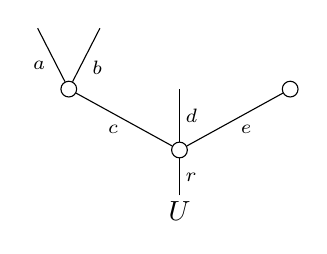
\begin{tikzpicture}[auto,grow=up, level distance = 2.2em,
            every node/.style={font=\scriptsize,inner sep = 2pt}]%
            \tikzstyle{level 2}=[sibling distance=4em]%
            \tikzstyle{level 3}=[sibling distance=2.25em]%
            \node [font=\normalsize] {$U$}
            child{node [dummy] {}
              child{node [dummy] {}
                edge from parent node [swap] {$e$}
              }
              child{edge from parent node [swap] {$d$}}
              child{node [dummy] {}
                child{edge from parent node [swap] {$b$}}
                child{edge from parent node {$a$}}
                edge from parent node {$c$}
              }
              edge from parent node [swap] {$r$}
            };        
      \end{tikzpicture}
\end{equation}
Edges with no vertices $\circ$ above them are called \textit{leaves}, the unique bottom edge is called the \textit{root},
and edges that are neither are called \textit{inner edges};
in the example above, $a$ and $b$ are the leaves, $r$ is the root, and $c$ and $e$ are inner edges.
The sets of edges, inner edges, leaves, and vertices of a tree $U$ are denoted $\boldsymbol{E}(U)$, $\boldsymbol{E}^i(U)$, $\boldsymbol{V}(T)$, and $\boldsymbol{V}(U)$ respectively.
% If an edge $t$ is pictorally above\footnote{While the following notation may seem backwards, $\leq_d$ flows in the direction of composition.} (or equal to) an edge $s$, we write $t \leq_d s$.

\begin{notation}
      We write $C_n$ to denote the \textit{$n$-corolla}, the unique (up to isomorphism) tree with
      $|\boldsymbol{V}(C_n)| = 1$ and $|\boldsymbol{L}(C_n)|=n$.
      Additionally, we write $\eta$ for the \textit{stick} tree, the unique tree with $|\boldsymbol{V}(\eta)| = 0$.

      Given any $v \in |\boldsymbol{V}(U)|$, we write $U_v$ for the sub-diagram of $U$
      consisting of the vertex $v$ and any adjacent edges.
\end{notation}


A map of trees $\phi \colon U \to V$ is defined to be
a map of edge sets $\phi \colon \boldsymbol{E}(S) \to \boldsymbol{E}(T)$
which preserves the incidence relations in an intuitive sense
(see e.g. \cite[\S 2.1]{BP_edss} for a rigorous definition).
% in the following intuitive sense:
% If $U$ is a corolla with leaves $\set{e_1,\dots, e_n}$ and root $e_0$,
% we first require that $\phi(e_i) \leq_d \phi(e_0)$ and $\phi(e_i) \not\leq_d \phi(e_j)$ for all $i \geq j > 0$.
% Moreover, consider the sub-diagram $V_U$ of $V$ where we chop of all vertices and edges above $\phi(e_i)$ and below $\phi(e_0)$;
% $\phi$ is a map of trees iff the set of leaves of this sub-diagram is precisely $\set{\phi(e_1), \dots, \phi(e_n)}$.
% For general trees $U$, $\phi$ is a map of tree iff every restricted map $U_v \to V$ is a map of trees.

\begin{example}
      \label{TREEMAP_EX}
      The labels on the edges of the tree diagrams below indicate a map to $\boldsymbol{E}(U)$ with $U$ defined as in \eqref{eq:TREE}.
      The maps determined by four leftmost trees are maps of trees, while the rightmost is not.
      \begin{equation}
            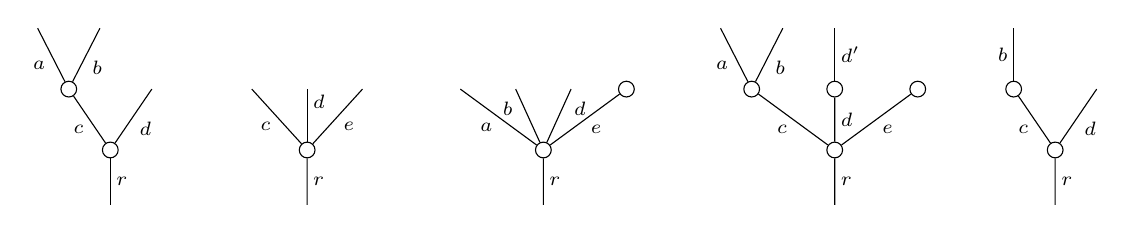
\begin{tikzpicture}[auto, grow=up, level distance = 2.2em,
                  every node/.style={font=\scriptsize,inner sep = 2pt}]
                  \tikzstyle{level 2}=[sibling distance=3em]%
                  \tikzstyle{level 3}=[sibling distance=2.25em]%
                  \node at (0,0) {} % {$T \setminus \set{e}$}
                  child{node [dummy] {}
                    child{edge from parent node [swap] {$d$}}
                    child{node [dummy] {}
                      child{edge from parent node [swap] {$b$}}
                      child{edge from parent node {$a$}}
                      edge from parent node {$c$}
                    }
                    edge from parent node [swap] {$r$}
                  };
                  \tikzstyle{level 2}=[sibling distance=2em]%
                  \node at (2.5,0) {} % {$\partial_{u,v}T$}
                  child{node [dummy] {}
                    child{edge from parent node [swap] {$e$}}
                    child{edge from parent node [swap,near end] {$d$}}
                    child{edge from parent node {$c$}}
                    edge from parent node [swap] {$r$}
                  };
                  \node at (5.5,0) {} % {$\partial_v(T \setminus \set{c})$}
                  child{node [dummy] {}
                    child{node [dummy] {}
                      edge from parent node [swap] {$e$}
                    }
                    child{edge from parent node [swap, very near end] {$d$}}
                    child{edge from parent node [very near end] {$b$}}
                    child{edge from parent node {$a$}}
                    edge from parent node [swap] {$r$}
                  };
                  \tikzstyle{level 2}=[sibling distance=3em]%
                  \node at (9.2,0) {} % {$\sigma_d T$}
                  child{node [dummy] {}
                    child{node [dummy] {}
                      edge from parent node [swap] {$e$}
                    }
                    child{node [dummy] {}
                      child{edge from parent node [swap] {$d'$}}
                      edge from parent node [swap] {$d$}
                    }
                    child{node [dummy] {}
                      child{edge from parent node [swap] {$b$}}
                      child{edge from parent node {$a$}}
                      edge from parent node {$c$}
                    }
                    edge from parent node [swap] {$r$}
                  };                    
                  \node at (12,0) {}
                  child{node [dummy] {}
                    child{edge from parent node [swap] {$d$}}
                    child{node [dummy] {}
                      child{edge from parent node {$b$}}
                      edge from parent node {$c$}
                    }
                    edge from parent node [swap] {$r$}
                  };
            \end{tikzpicture}
      \end{equation}
\end{example}

A map of trees $\phi \colon U \to V$ is called
\begin{itemize}
\item a \textit{tall map} if
      $\phi(\boldsymbol{L}(U)) = \boldsymbol{L}(V)$ and $\phi(r_U) = r_V$
      for $r_{(-)}$ denoting the root edge.
\item a \textit{face map} if it is injective on edges;
      an \textit{inner face} if it is also tall, and
      an \textit{outer face} if it does not factor through a non-isomorphism inner face map.
\item a \textit{degeneracy} if is surjective on edges and preserves leaves
      (and hence is tall).
\end{itemize}

Heuristically, inner face maps split vertices to create new inner edges in $U$,
outer face maps glue on new vertices,
and degeneracies collapse unary vertices.
\begin{example}
      In Example \ref{TREEMAP_EX},
      the first map is an inner face, the second an outer face, the third is a general face, while the fourth is a degeneracy.
\end{example}

\begin{proposition}[{\cite[Prop. 2.2]{BP_edss}}]
      An arrow of trees $\phi \colon U \to V$ has a factorization, unique up to unique isomorphisms,
      \begin{equation}
            \label{TREEFACT_EQ}
            U \xrightarrow{\phi^-} U' \xrightarrow{\phi^i} U'' \xrightarrow{\phi^o} V
      \end{equation}
      as a degeneracy followed by an inner face map followed by an outer face map.
\end{proposition}


\begin{remark}
      For technical ease, we will assume that all trees $U$ are equipped with a \textit{planar} structure.
      % a well-behaved total order on $\boldsymbol{E}(U)$ which extends $\leq_d$.
      Heuristically, a planar structure is equivalent to choosing a 2D-representation of the tree diagram.
      In particular, the factorization from \eqref{TREEFACT_EQ} is actually unique if we demand that $\phi^i$ and $\phi^o$ are planar.
      Moreover, the subtrees of $U$ correspond bijectively to the planar outer faces of $U$.
      
      A rigorous definition and more discussion can be found in \cite[\S 3.1]{BP_geo}.
\end{remark}

\begin{definition}
      We let $\Omega$ denote a fixed full subcategory of trees and (non-planar) arrows
      such that the subcategory of planar maps in skeletal (i.e. if two trees are planar isomorphic, they are in fact equal and said isomorphism is the identity).
\end{definition}

\begin{remark}
      The subcategory of corollas and isomorphisms is isomorphic to the category $\Sigma$ of standard finite ordered sets and isomorphisms,
      and we will conflate the two notions and notations.
\end{remark}

\begin{notation}
      \label{LR_NOT}
      For each $U \in \Omega$, there exists a unique corolla $\mathsf{lr}(U) \in \Sigma$ equipped with a planar tall map $\mathsf{lr}(U) \to U$,
      which we call the \textit{leaf-root} of $U$.
\end{notation}


Next, we consider categories of (colored) forests (cf. \cite[Defn. 2.56]{BP_HGOP}).

\begin{definition}
      The category $\Phi$ of \textit{forests} is the coproduct completion of the category $\Omega$ of trees:
      objects are finite tuples $F = (F_i)_{i \in I}$ with $F_i \in \Omega$,
      and an arrow $\phi \colon (F_i)_{i \in I} \to (F'_j)_{j \in J}$ is given by
      a map $\phi \colon I \to J$ and
      maps $\phi_i \colon F_i \to F'_{\phi(i)}$ for all $i \in I$.
     
      The sets $\boldsymbol{E}(F)$, $\boldsymbol{E}^i(F)$, $\boldsymbol{L}(F)$, $\boldsymbol{V}(F)$ generalize immediately.
      Moreover, we call a map $\phi \colon F \to F'$ an \textit{(inner, outer) face map} or a \textit{degeneracy} iff
      $\phi_i$ is so in $\Omega$ for all $i \in I$.
\end{definition}

Finally, we may color the edges of any forest or tree.
\begin{definition}            
      Let $\mathfrak C$ be a set of colors.
      The category $\Phi_{\mathfrak C}$ of \textit{$\mathfrak C$-colored forests} has
      \begin{itemize}
      \item objects pairs $\vect F = (F, \mathfrak c)$ with
            $F \in \Phi$ a forest and
            $\mathfrak c \colon \boldsymbol{E}(F) \to \mathfrak C$ a coloring of its edges.
      \item arrows $\vect F = (F, \mathfrak c) \to (F', \mathfrak c') = \vect{F'}$ maps
            $\rho\colon F \to F'$ in $\Phi$ such that $\mathfrak c = \mathfrak c' \rho$.
      \end{itemize}      

      These naturally assemble into category $\Phi_\bullet \to \Set$ fibered over $\Set$.
      Moreover, we denote by
      $\Phi_\bullet^0 \subseteq \Phi_\bullet$
      the wide subcategory of those arrows whose maps on uncolored forests are outer faces.
\end{definition}

\subsection{The category of equivariant trees}

We briefly recall the category $\Omega_G$ of equivariant trees, which encodes the combinatorics of compositions of norm maps;
a more thourough discussion can be found in \cite{Per18} or \cite[\S 2]{BP_edss}.

We begin with an explicit example.
Let $G = D_{8} = \set{1,\sigma,\sigma^2,\sigma^3, \rho, \sigma\rho, \sigma^2\rho, \sigma^3\rho}$
be the dihedral group with 8 elements,
and $L \leq K \leq H \leq G$ denote the subgroups
$H = \langle \sigma^2,\rho \rangle$, $K = \langle \sigma^2 \rangle$, $L = \**$.
Then we have a $G$-tree $T$ as below,
with the \textit{expanded representation} given by the two trees on the left below,
and the \textit{orbital representation} given by the single decorated tree on the right.
\begin{equation}
      \label{GTREE_EQ}
      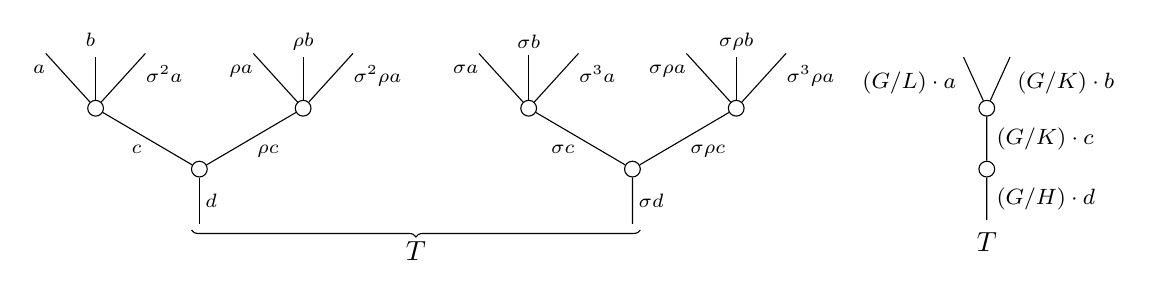
\begin{tikzpicture}[auto,grow=up, level distance = 2.2em,
            every node/.style={font=\scriptsize,inner sep = 2pt}]%
            \tikzstyle{level 2}=[sibling distance=7.5em]%
            \tikzstyle{level 3}=[sibling distance=2em]%
            \node at (5.5,0){}%	
            child{node [dummy] {}%
              child{node [dummy] {}%
                child{node {}%
                  edge from parent node [swap,very near end] {$\sigma^3 \rho a$}}%
                child[level distance = 2.4em]{node {$\sigma\rho b$}}%
                  % edge from parent node [swap,near end] {$\sigma\rho b$}}%
                child{node {}%
                  edge from parent node [very near end] {$\sigma \rho a$}}%
                edge from parent node [swap] {$\sigma \rho c$}}%
              child{node [dummy] {}%
                child{node {}%
                  edge from parent node [swap,very near end] {$\sigma^3 a$}}%
                child[level distance = 2.4em]{node {$\sigma b$}}%
                % edge from parent node [swap,near end] {$\sigma b$}}%
                child{node {}%
                  edge from parent node [very near end] {$\sigma a$}}%
                edge from parent node  {$\sigma c$}}%
              edge from parent node [swap] {$\sigma d$}};%
            \node at (0,0){}%	
            child{node [dummy] {}%
              child{node [dummy] {}%
                child{node {}%
                  edge from parent node [swap,very near end] {$\sigma^2\rho a$}}%
                child[level distance = 2.4em]{node {$\rho b$}}%
                % edge from parent node [swap,near end] {$\rho b$}}%
                child{node {}%
                  edge from parent node [very near end] {$\rho a$}}%
                edge from parent node [swap] {$\rho c$}}%
              child{node [dummy] {}%
                child{node {}%
                  edge from parent node [swap,very near end] {$\sigma^2 a$}}%
                child[level distance = 2.4em]{node {$b\phantom{j}$}}%
                % edge from parent node [swap,near end] {$b\phantom{j}$}}%
                child{node {}%
                  edge from parent node [very near end] {$a$}}%
                edge from parent node  {$c$}}%
              edge from parent node [swap] {$d$}};%
            \begin{scope}[every node/.style={font=\footnotesize}]%
                  \node at (10,0) {}
                  child{node [dummy] {}%
                    child{node [dummy] {}%
                      child{node {}%
                        edge from parent node [swap,very near end] {$(G/K) \cdot b$}}%
                      child{node {}%
                        edge from parent node [very near end] {$(G/L) \cdot a$}}%
                      edge from parent node [right] {$(G/K) \cdot c$}}%
                    edge from parent node [right] {$(G/H) \cdot d$}};%
            \end{scope}%
            \draw[decorate,decoration={brace,amplitude=2.5pt}] (5.6,0) -- (-0.1,0) node[midway,inner sep=4pt,font=\normalsize]{$T$}; %
            \node at (10,-0.15) [font=\normalsize] {$T$}; 
     \end{tikzpicture}%
\end{equation}
The expanded representation is a planar representation of the $G$-sets of edges and vertices, equipped with names for the edges which indicate the group action on the set of edges (and hence also vertices).
In the orbital representation, each edge indicates an orbit worth of edges from the expanded representation,
and is labeled by the appropriate transitive $G$-set.

In general, we have the following.
\begin{definition}
      Let $\Phi^G$ denote the category of forests with $G$-action. 
      The category $\Omega_G$ of \textit{$G$-trees} is the full subcategory of $\Phi^G$ spanned by those $G$-forests whose
      $G$-set of roots has a transitive $G$-action.
\end{definition}

\begin{remark}
      We denote objects in $\Omega_G$ by $T = (T_i)_{i \in I}$ with $I$ a transitive $G$-set and $T_i$ trees.
      Alternatively, any choice of component $T_{\**}$ has a stabilizer $H \leq G$, and then we have a decomposition
      $T \simeq G \cdot_H T_{\**}$.
      Finally, if $\Gamma \leq G \times \Aut(T_{\**})$ is the graph subgroup encoding the $H$-action on $T_{\**}$, we have
      $T \simeq G \cdot T_{\**}/\Gamma$.
\end{remark}
% Any $T \in \Omega_G$ has several equivalent descriptions:
% \begin{enumerate}
% \item By definition, $T$ consists of a tuple $(T_i)_{i \in I}$ of trees in $\Omega$, equipped with a compatible $G$-action
%       which makes $I$ a transitive $G$-set.
% \item Alternatively, this data is given by a functor $T: G \ltimes I \to \Omega$.
% \item Any component $T_{\**}$ of $T$ is stabilized by some subgroup $H \leq G$, and $T$ may be described as an induction
%       $T \simeq G \cdot_H T_{\**}$.
% \item Similarly, fixing a component $T_{\**}$, let $\Gamma \leq G \times \Aut(T_{\**})$ denote the graph subgroup encoding the $H$-action on $T_{\**}$;
%       $T$ may then be described as the quotient $T \simeq G \cdot U / \Gamma$.
% \end{enumerate}
For $T \in \Omega_G$, we write
$\boldsymbol{E}_G(T) = \boldsymbol{E}(T)/G$, $\boldsymbol{E}^i_G(T) = \boldsymbol{E}^i(T)/G$, $\boldsymbol{V}_G(T) = \boldsymbol{V}(T)/G$
for the set of \textit{edge orbits}, \textit{inner edge orbits}, and \textit{$G$-vertices}, respectively.

\begin{remark}
      $\Omega_G$ is fibered over the \textit{orbit category} $\mathsf O_G$ of transitive $G$-sets and $G$-maps,
      by the functor which sends a $G$-tree $T = (T_i)_{i \in I}$ to its $G$-set of roots $\underline{r}_T \simeq I$.
\end{remark}


\begin{remark}
      The two representations of $G$-trees from \eqref{GTREE_EQ} play complementary roles in our analysis:
      the expanded representation displays all of the relevant edge information, and thus is often useful for describing maps between $G$-trees;
      conversely, the orbital representation compactly displays the relevant data for composing norm maps of operads (e.g. {\color{blue} Example \ref{GTREENORM_EX}}).
\end{remark}

As in $\Omega,$ we can describe maps $\phi = (\varphi, (\phi_j))\colon (S_j)_{j \in J} \to (T_i)_{i \in I}$ between $G$-trees as being built out of a few types of maps.
In each fiber over $\mathsf O_G$, we say $\phi$ is an
\textit{(inner, outer) face map}, \textit{degeneracy map}, \textit{tall map}, or \textit{planar map} if
$\phi_j \colon S_j \to T_{\varphi(j)}$ is so for some (and thus all) $j \in J$.
The cartesian arrows are a new type of map, dubbed \textit{quotients},
which act as twisted fold maps on the forest components;
explicitly, $\phi$ is a quotient iff $\phi_j \colon S_j \to T_{\varphi(j)}$ is an isomorphism for some (and thus all) $j \in J$.

We give a minimal example of a quotient below;
fuirther discussion and examples can be found at \cite[Remark 5.49]{Per18}.
\begin{example}
      Let $G = \mathbb Z/ 2\mathbb Z$ be the cyclic group with two elements.
      We have the following quotient map on $G$-corollas,
      where $\alpha \mapsto a$, $\alpha^- \mapsto -a$, $\beta \mapsto b$, $\gamma \mapsto c$.
      \[
            \begin{tikzpicture}[grow=up,auto,level distance=2.4em,
                  every node/.style={font=\scriptsize,inner sep = 2pt}]%
                  \tikzstyle{level 2}=[sibling distance=4em]%
                  \begin{scope}[every node/.style={font=\footnotesize}]%
                        \node at (0,0) {}
                        child{node [dummy] {}
                          child{edge from parent node [swap,near end] {$G/e+\alpha^{-}$}}
                          child{node {$G/e + \beta$}}
                          child{edge from parent node [near end] {$G/e + \alpha$}}
                          edge from parent node [swap] {$G/2 + \gamma$}
                        };
                        % 
                        \node at (4.8,1) {$\xrightarrow{\qquad \qquad}$};
                        % 
                        \node at (8,0) {}
                        child{node [dummy] {}
                          child{edge from parent node [swap] {$G/G + b$}}
                          child{edge from parent node {$G/e+a$}}
                          edge from parent node [swap] {$G/G+c$}
                        };
                  \end{scope}%
                  \begin{scope}[level distance=2em]
                        \tikzstyle{level 2}=[sibling distance=3em]%
                        \node at (-2,-2.5) {}
                        child{node [dummy] {}
                          child{edge from parent node [swap, near end] {$\alpha^{-}$}}
                          child{edge from parent node [swap, very near end] {$\beta$}}
                          child{edge from parent node [near end] {$\alpha$}}
                          edge from parent node [swap] {$\gamma$}
                        };
                        \node at (2,-2.5) {}
                        child{node [dummy] {}
                          child{edge from parent node [swap, near end] {$-\alpha^{-}$}}
                          child{edge from parent node [swap, very near end] {$-\beta$}}
                          child{edge from parent node [near end] {$-\alpha$}}
                          edge from parent node [swap] {$-\gamma$}
                        };
                        \node at (4.8,-1.7) {$\xrightarrow{ \qquad \qquad}$};
                        \node at (8,-2.5) {}
                        child{node [dummy] {}
                          child{edge from parent node [swap, near end] {$-a$}}
                          child{edge from parent node [swap, very near end] {$b$}}
                          child{edge from parent node [near end] {$a$}}
                          edge from parent node [swap] {$c$}
                        };                  
                  \end{scope}
                  \draw[decorate,decoration={brace,amplitude=2.5pt}] (2.1,-2.5) -- (-2.1,-2.5) node[midway,inner sep=4pt,font=\normalsize]{$S$}; %
                  \node at (8,-2.65) [font=\normalsize] {$T$};
                  \node at (8,-.15) [font=\normalsize] {$T$};
                  \node at (0,-.15) [font=\normalsize] {$S$};
            \end{tikzpicture}
      \]
\end{example}

\begin{corollary}[{cf. \cite[Remark 5.49]{Per18}}]
      A map $\phi \colon S \to T$ in $\Omega_G$ has a factorization, unique up to unique isomorphism,
      \[
            S \xrightarrow{\phi^-} S' \xrightarrow{\phi^i} S'' \xrightarrow{\phi^o} q^{\**}T \xrightarrow{q} T
      \]
      as, in order: a degeneracy $\phi^-$, an inner face $\phi^i$, an outer face $\phi^o$, and a quotient $q$.
\end{corollary}

\begin{definition}
      We denote by $\Omega_G^0 \subseteq \Omega_G$ the wide subcategory of $G$-trees and quotient maps.
      Further, we write $\Sigma_G \subseteq \Omega_G^0$ for the full subcategory spanned by \textit{$G$-corollas} and quotient maps,
      where $C \in \Omega_G$ is a $G$-corolla if $|\boldsymbol{V}_G(C)| = 1$.

      We note that for any choice of decomposition $C \simeq G \cdot_H C_{\**}$, $\boldsymbol{L}(C_{\**})$ is an $H$-set,
      and the assignment $C \mapsto \boldsymbol{L}(C_{\**})$ provides a bijection between
      isomorphism classes of objects in $\Sigma_G$ and
      isomorphism classes of $H$-sets for $H \leq G$.
\end{definition}
      
\begin{notation}
      \label{LRG_NOT}
      As in Notation \ref{LR_NOT}, 
      for any $T = (T_i)_{i \in I} \in \Omega_G$ there exists a unique $G$-corolla $\mathsf{lr}(T) \in \Sigma_G$ equipped with a planar tall map $\mathsf{lr}(T) \to T$
      called the \textit{leaf-root} of $T$.
      Explicitly, $\mathsf{lr}(T) = (\mathsf{lr}(T_i))_{i \in I}$.
\end{notation}

Finally, we have an alternative definition of the ``faces'' of a $G$-trees, as detected by regular trees $U \in \Omega$.
\begin{definition}
      Let $T = (T_i) \in \Omega_G$ be a $G$-tree.
      An \textit{(outer) face} of $T$ is an (outer) face map $U \to T_i$ from some $U \in \Omega$ to a component $T_i$ of $T$.
      A face of $T$ is called \textit{planar} if the map $U \to T_i$ preserves the planar order.

      Let $\mathsf{Face}(T)$ denote the $G$-poset of planar faces of $T$,
      and let $\mathsf{Face}_{SC}(T) \subseteq \mathsf{Face}(T)$ denote the sub-poset spanned by the planar outer faces of $T$ with no inner edges.
\end{definition}



\subsection{Equivariant dendroidal sets}
\label{EDS_SEC}

We consider the presheaf category 
$
\dSet^G = \Fun(G \times \Omega^{op}, \Set),
$
of \textit{equivariant dendroidal sets}.
There is a natural fully-faithful inclusion
\[
      \Omega[-] \colon \Omega_G \longto \dSet^G,
      \qquad
      T = (T_i) \longmapsto \Omega[T] = \coprod \Omega[T_i]
      % \simeq G \cdot_H \Omega[T_{\**}].
      % \simeq \left(G \cdot \Omega[T_{\**}] \right) / N
\]
extending the Yoneda embedding $\Omega \times G \into \dSet^G$.
These $\Omega[T]$ allow us to probe presheaves $X \in \dSet^G$ by $G$-trees and detect ``norm map'' information 
(e.g. \cite[Example 4.9]{Per18}, {\color{blue} Example}).
As such, they will be the building blocks of several fundamental definitions (cf. \cite[\S 6]{Per18}), generalizing the standard presheaf constructions.

\begin{definition}
      \label{DSETPRESHEAF_DEF}
      For $T = (T_i) \in \Omega_G$, let $\partial \Omega[T] \subseteq \Omega[T]$ denote the \textit{boundary}
      \begin{equation}
            \partial \Omega[T] = \coprod \partial \Omega[T_i]
            = \mathop{\colim}\limits_{U \in \mathsf{Face}(T), U \neq T} \Omega[U]
            = \bigcup_{U \in \mathsf{Face}(T), U \neq T} \Omega[U]
      \end{equation}
      and the \textit{boundary inclusions} are all maps of the form
      $\partial \Omega[T] \to \Omega[T]$, $T \in \Omega_G$.

      Next, given any sub-$G$-set $E \subseteq_G \boldsymbol{E}(T)$, we write $E_i = E \cap \boldsymbol{E}(T_i)$, and let
      $\Lambda^{E}[T] \subseteq \partial \Omega[T] \subseteq \Omega[T]$,
      denote the associated \textit{$G$-inner horn}
      \begin{equation}
            \label{GINNERHORN_EQ}
            \Lambda^{E}[T] = \coprod \Lambda^{E_i}[T_i]
            = \mathop{\colim}\limits_{U \in \mathsf{Face}(T), (T_i \setminus E_i) \not\into U} \Omega[U]
            = \bigcup_{U \in \mathsf{Face}(T), (T_i \setminus E_i) \not\into U} \Omega[U]
      \end{equation}
      and the \textit{$G$-inner horn inclusions} are all maps of the form
      $\Lambda^{E}[T] \to \Omega[T]$, $T \in \Omega_G$ and $E \subseteq_G \boldsymbol{E}(T)$.

      Finally, we define the \textit{Segal core} of $T$ to be
      \begin{equation}
            \label{eq:SC}
            Sc[T] = \coprod Sc[T_i]
            = \mathop{\colim}\limits_{U \in \mathsf{Face}_{SC}(T)} \Omega[U]
            = \bigcup_{U \in \mathsf{Face}_{SC}(T)} \Omega[U],
      \end{equation}
      and the \textit{Segal core inclusions} to be those maps in $\dSet^G$ of the form
      $Sc(T) \to \Omega[T]$.
\end{definition}


\begin{remark}
      For $T \in \Omega_G$, any decomposition $T \simeq G \cdot_H T_{\**}$ with $T_{\**} \in \Omega^H$ yields
      \[
            \Omega[T] \simeq G \cdot_H \Omega[T_{\**}],
            \qquad
            \partial\Omega[T] \simeq G \cdot_H \partial \Omega[T],
            \qquad
            \Lambda^{Ge}[T] \simeq G \cdot_H \Lambda^{E_{\**}}[T_{\**}],
            \qquad.
            Sc[T] \simeq G \cdot_H Sc[T_{\**}]
      \]
      % where $E_{\**} = E \cap \boldsymbol{E}(T_{\**})$.
\end{remark}

\begin{notation}
      For $X \in \dSet^G$ and $A$ an $H$-set with $|A|=n$, we write
      \[
            X(A) = X(C_n)^{\Gamma_A} = \Hom_{\dSet^G}(\Omega[C_A],X)
      \]
      for $\Gamma_A \leq G \times \Sigma_n$ the graph subgroup encoding the $H$-action on $A$ and
      $C_A \in \Omega_G$ a $G$-corolla associated to the $H$-set $A$.
\end{notation}

\begin{definition}
      A presheaf $X \in \dSet^G$ is called a \textit{$G$-$\infty$-operad} if $X \to \**$ has the right lifting property with respect to all generating $G$-inner horn inclusions.
      By {\color{blue} citation}, this is equivalent to $X$ having the right lifting property with respect to all Segal core inclusions.
\end{definition}
Intuitively,
$G$-$\infty$-operads are operads with weak composition laws for norm maps:
\begin{example}
      We recall the setup of \eqref{GTREE_EQ}, with $G = D_8$, $H = \langle \sigma^2,\rho \rangle$, $K = \langle \sigma^2 \rangle$, $L = \**$, and $T$ the given tree diagram.
      Let $X \in \dSet^G$. Then we have natural solid arrows
      \[
            \begin{tikzcd}
                  X(H/K) \times X(K/L \amalg K/K) \arrow[r, start anchor = east, end anchor = west, dashed, bend left, shift left]
                  &
                  \Hom_{\dSet^G}(\Omega[T], X) \arrow[l, shift left] \arrow[r]
                  &
                  X(H/L \amalg H/K)
            \end{tikzcd}
      \]
      given by the presheaf structure,
      If $X$ is a $G$-$\infty$-operad, there exists a dashed section (possibly many) as written,
      and the composite map provides a choice of a composition law.
      providing a choice of composition.     
\end{example}





The maps from Definition \ref{DSETPRESHEAF_DEF} form the basis for a model structure on $\dSet^G$.

\begin{definition}
      The class of \textit{$G$-normal monomorphisms}
      is the smallest saturated\footnote{A class of maps is \textit{saturated} if it is closed under pushouts, retracts, and transfinite compositions.}
      class of maps containing the boundary inclusions $\partial \Omega[T] \into \Omega[T]$ for all $T \in \Omega_G$.
      Dually, a map is called a \textit{trivial fibration} if it has the right lifting property with respect to the $G$-normal monomorphisms.
      
      The class of \textit{$G$-inner anodyne extensions} is the smallest saturated class of maps containing the generating $G$-inner horn inclusions.
\end{definition}

\begin{theorem}[{\cite[Thm 2.1, Thm 8.22]{Per18}}]
      There exists a model structure on $\dSet^G$ such that
      \begin{itemize}
      \item cofibrations are $G$-normal monomorphisms,
      \item fibrant objects are $G$-$\infty$-operads,
      \item fibrations between fibrant objects are precisely the maps $X \to Y$ such that the functors associated to each of the fixed-point homotopy categories $\tau j^{\**}(X^H \to Y^H)$ are isofibrations of categories for all $H \leq G$.
      \item weak equivalences are the smallest class of maps closed under 2-out-of-3 which
            contains the $G$-inner anodyne extensions and trivial fibrations.
      \end{itemize}
\end{theorem}







\subsection{Equivariant simplicial operads}

We now recall our main objects of study; further details and exposition can be found in \cite[\S 2]{BP_HGOP}.

We denote by $\mathsf{sOp}^G$ the category of \textit{equivariant colored simplicial operads}, also know as \textit{$G$-objects in simplicially enriched muliticategories}.
These will be given as algebra over a monad $\mathbb F$ on the category of equivariant symmetric sequences.

We begin non-equivariantly.
\begin{definition}
      Let $\mathfrak C$ be a set. A \textit{$\mathfrak C$-signature} is a tuple
      $\vect C = (\mathfrak c_1, \dots, \mathfrak c_n; \mathfrak c_0) = (\mathfrak c_i)_{0 \leq i \leq n}$ in $\mathfrak C^{\times n+1}$.
      The \textit{$\mathfrak C$-symmetric category} is the category denoted $\Sigma_{\mathfrak C}$ with
      objects $\mathfrak C$-signatures and
      arrows $\vect C = (\mathfrak c_i)_{0 \leq i \leq n} \to (\mathfrak d_j)_{0 \leq j \leq m} = \vect D$
      given by $\sigma \in \Sigma_n$ such that $\mathfrak c_{\sigma i} = \mathfrak d_i$ if $n = m$, with no arrows otherwise.
\end{definition}

The category $\mathsf{sSym}$ of \textit{simplicial symmetric sequences} has
objects pairs $(\mathfrak C, X)$ with $X \colon \Sigma_{\mathfrak C}^{op} \to \sSet$,
and arrows $(\mathfrak C, X) \to (\mathfrak D, Y)$ are pairs $(\phi, \Phi)$ with
$\phi \colon \mathfrak C \to \mathfrak D$ a $G$-map of colors and
$\Phi \colon X \Rightarrow Y \phi$ a natural transformation.

$\sSym$ is naturally fibered over $\Set$,
and the free operad monad $\mathbb F$ yields an adjunction
\[
      \sSym \overset{\mathbb F}{\rightleftarrows} \sOp
\]
which is also fibered over $\Set$.

By abstract nonsense, this lifts to a monadic adjunction on the categories of $G$-objects, as on the left below, fibered over $\Set^G$.
\[
      \sSym^G \overset{\mathbb F}{\rightleftarrows} \sOp^G
      \qquad
      \sSym^G_{\mathfrak C} \overset{\mathbb F_{\mathfrak C}}{\rightleftarrows} \sOp^G_{\mathfrak C}
\]
We also have the induced monad $\mathbb F_{\mathfrak C}$ on the fibers,
where $\sSym^G_{\mathfrak C} \simeq \Fun(G \ltimes \Sigma_{\mathfrak C}^{op}, \sSet)$ for
$G \ltimes \Sigma_{\mathfrak C}^{op}$ denoting category fibered over $G$ encoding the $G$-action on $\Sigma_{\mathfrak C}^{op}$ (e.g. \cite[Example 2.13]{BP_HGOP}).

For more information on fibered adjunctions, see \cite[\S 2.2]{BP_HGOP}.


\begin{notation}
      We will often simply write $\O$ to denote an object in $\sOp^G$,
      letting $\mathfrak C_\O \in \Set^G$ denote the associated $G$-set of colors of $\O$.
\end{notation}

\begin{notation}
      Let $\mathfrak C$ be a $G$-set, and $\vect C = (\mathfrak c_1, \dots, \mathfrak c_n; \mathfrak c_0)$ a $\mathfrak C$-signature.
      Then $\Aut_{G \ltimes \Sigma_{\mathfrak C}}(\vect C) \leq G \times \Sigma_n$,
      and for $\Gamma \leq G \times \Sigma_n$, we say \textit{$\Gamma$ stabilizes $\vect C$} if $\Gamma \leq \Aut(\vect C)$.

      In particular, $\O(\vect C)$ has an action by $\Gamma$ for all $\Gamma$ which stabilize $\vect C$.
\end{notation}

{\color{OliveGreen} % ------------------------------ OLIVE GREEN ------------------------------
  \todo[inline]{the following remark probably won't go here, but instead this idea will be stated in the introduction}
  \begin{remark}
        For $\mathfrak C = \**$ and $\Gamma \leq G \times \Sigma_n$ a $G$-graph subgroup corresponding to some homomorphism $H \to \Sigma_n$,
        $\O(n)^{\Gamma}$ corresponds to a space of \textit{norm multiplications}:
        For any $\O$-algebra $E$, the action map descends to an $H$-equivariant map
        \[
              \O(n)^{\Gamma} \longto \Hom^H(N^\Gamma E, E)
        \]
        where $N^\Gamma E = \alpha^{\**}E^{\times n}$ is the \textit{norm of $E$}, with $\alpha \colon H \xrightarrow{\simeq} \Gamma$ the isomorphism of groups.
        Equivalently, $N^\Gamma E \simeq N^A E$ for $A$ the $H$-set structure on $\set{1,\dots, n}$ induced by $\Gamma$.

        Thus, we refer to the fixed-point spaces $\O(n)^\Gamma$,
        and more generally $\O(\vect C)^\Gamma$ for $\Gamma$ a graph subgroup which stabilizes the $\mathfrak C_\O$-signature $\vect C$,
        as \textit{spaces of norm maps}.
  \end{remark}
} % ---------------------------------- OLIVE GREEN ----------------------------------------------

Generalizing the work of \cite{Ber07b,CM13b}, in \cite{BP_HGOP} we show that
the category of equivariant simplicial operads is equipped with a Dwyer-Kan model structure,
where weak equivalences are homotopically essentially surjective maps which have the same homotopy types for every space of norm maps $\O(\vect C)^\Gamma$.

% First, the fibers $\sOp^G_{\mathfrak C}$ have a model structure transfered from $\sSym^G_{\mathfrak C}$ by \cite[Thm. I]{BP_HGOP},
% where a map $X \to Y$ is a weak equivalence (resp. fibration) iff
% $X(\vect C) \to Y(\vect C)$ is a $G$-graph weak equivalence (resp. fibration) in $\sSet^{\Aut_{G \ltimes \Sigma_{\mathfrak C}^{op}}(\vect C)}$

% Second, these model structures on $\sOp_{\mathfrak C}^G$ assemble into a single model structure on all operads.
\begin{notation}
      We recall two natural right adjoints:
      \[
            \sOp^G \xrightarrow{\pi_0}
            \Op^G \xrightarrow{j^{\**}}
            \Cat
      \]
      where $\pi_0(\mathfrak C, \O) = (\mathfrak C, \pi_0 \O)$ with $\pi_0\O(\vect C) = \pi_0\left(\O(\vect C)\right)$,
      and $j^{\**}$ forgets all non-unary operations.
\end{notation}

\begin{theorem}[{cf. \cite[Thm. III, Prop. 4.78]{BP_HGOP}}] % ISOFIBHARD PROP
      The category $\sOp^G$ is equipped with a cofibrantly generated model structure where the weak equivalences (resp. fibrations) are those maps
      $F \colon \O \to \P$ such that
      \begin{itemize}
      \item the induced maps
            \begin{equation}
                  \label{DKEQUIV_EQ}
                  \O(\mathfrak c_1, \dots, \mathfrak c_n; \mathfrak c_0)^\Gamma \longto \P(F \mathfrak c_1, \dots, F \mathfrak c_n; F \mathfrak c_0)^\Gamma
            \end{equation}
            is a Kan equivalence (resp. Kan fibration) in $\sSet$
            for all $\mathfrak C_\O$-signatures $\vect C = (\mathfrak c_1, \dots, \mathfrak c_n; \mathfrak c_0)$
            and all \textit{graph subgroups} $\Gamma \leq G \times \Sigma_n$ which stabilize $\vect C$.
      \item the induced maps of categories
            \[
                  j^{\**}\pi_0 \O^H \longto j^{\**}\pi_0 \P^H
            \]
            is essentially surjective (resp. an isofibration) for all $H \leq G$.
      \end{itemize}
\end{theorem}

\todo[inline]{come back}

Lastly, we have that cofibrant operads forget to cofibrant symmetric sequences.
\begin{definition}
      We say a map $\O \to \P$ in $\sOp^G_{\mathfrak C}$ is a \textit{$\Sigma$-cofibration}
      if the underlying map of $\mathfrak C$-colored symmetric sequences is a $G$-graph cofibration in $\sSym_{\mathfrak C}^G$. 
\end{definition}

\begin{proposition}[{cf. \cite[Prop. 3.63]{BP_HGOP}}]
      \label{SIGMAG_COF PROP}
      If $F \colon \O \to \P$ is a cofibration in $\Op^G_{\mathfrak C}(\V)$ and $\O$ is $\Sigma$-cofibrant,
      then $F$ is a $\Sigma$-cofibration.
      In particular, cofibrant operads are $\Sigma$-cofibrant.
\end{proposition}

\todo[inline]{come back - make sure this goes here}
Now, recall (e.g. \cite[Prop. 2.16]{Ste16}) that for any group $G$ and family of subgroups $\F$,
a map $K \to L$ in $\sSet^{G}_\F$ is an $\F$-cofibration iff $L_n \setminus K_n$ has isotropy in $\F$; i.e. for all $x \in L_n \setminus K-n$, $\Stab_{G}(x) \in \F$. 
% 
We also note the easy observation that for any set $A$ with an action of $G \times \Sigma$,
$A$ has isotropy in the family $\F^\Gamma$ of $G$-graph subgroups
iff
$A$ is $\Sigma$-free.
% 
Thus $K \to L$ in $\sSet^{G \times \Sigma}_{\F^\Gamma}$ is an $\F^\Gamma$-cofibration
iff
it forgets to a cofibration in the coarse model structure $\sSet^\Sigma_{proj}$.

More generally, if $\Lambda \leq G \times \Sigma$ and $\F^\Gamma_{\Lambda} = \F^\Gamma \cap \Lambda$,
then $K \to L$ in $\sSet^{\Lambda}_{\F^\Gamma_\Lambda}$ is an $\F^\Gamma_\Lambda$-cofibration
iff
it forgets to a cofibration in the coarse model structure $\sSet^{\pi_{\Sigma}\Lambda}_{proj}$.
      
All together, we conclude the following (cf. \cite[Remark 6.7]{Per18}, \cite[discussion before Thm. 2.31]{BP_edss}).

\begin{proposition}
      \label{SGS_COF_PROP}
      $X \to Y$ in $\mathsf{sSym}^G$ is a $G$-graph cofibration iff
      it forgets to a cofibration in $\mathsf{sSym}$.
      %
      % $\O \to \P$ in $\Op_\bullet^G(\sSet)$ is a $\Sigma_{\F^\Gamma}$-cofibration iff
      % it forgets to a $\Sigma$-cofibration in $\Op_\bullet(\sSet)$
      % (i.e. it forgets to a cofibration in $\Sym_\bullet(\sSet)$).
      %
      Consequently, $\O \in \sOp^G$ is $\Sigma$-cofibrant iff $\O(n)$ has a free $\Sigma_n$-action for all $n \geq 0$.
\end{proposition}

\subsubsection{Simplicial tensoring and generating (trivial) cofibrations}

To describe the generators of this model structure, we must recall two natural constructions:
\begin{enumerate*}
\item the free operad $\Omega(T)$ generated by a $G$-tree.
\item a (fiberwise) simplicial (co)tensoring of $\sOp^G$, and
\end{enumerate*}








% ------------------------------ construction on $\Omega(T)$ ------------------------------

We begin with $\Omega(T)$; more details can be found in \cite[\S 2.3.1]{BP_HGOP}). % {REPFUN_SEC}
Given $\vect C \in \Sigma_{\mathfrak C}$, we have a representable functor $\Sigma_{\mathfrak C}[\vect C] = \Sigma_{\mathfrak C}^{op}(\vect C, -)$ in $\Sym_{\mathfrak C}$..
More generally, for any $\mathfrak C$-colored forest $\vect F$, we define
\[
      \Sigma_{\mathfrak C}[\vect F] = \sideset{}{^{\mathfrak C}}\coprod_{v \in \boldsymbol{V}(F)} \Sigma_{\mathfrak C}[\vect F_v],
\]
where we highlight that the coproduct $\amalg^{\mathfrak C}$ is fibered, i.e. takes place in $\Sym_{\mathfrak C}$ rather than $\Sym_\bullet$.
This extends to functors
\[
      \Phi_\bullet^0 \xrightarrow{\Sigma_\bullet[-]} \Sym_\bullet
      \qquad
      \Phi_\bullet^{0,G} \xrightarrow{\Sigma_\bullet[-]} \Sym_\bullet^G
\]
which are fibered over $\Set$ and $\Set^G$, respectively.

We also recall the \textit{tautological coloring} functor $(-)^\tau \colon \Phi \to \Phi_{\bullet}$
which sends $F \in \Phi$ to $F^\tau \in \Phi_{\boldsymbol{E}(T)}$,
where $F^\tau = (F,\mathfrak t)$ is the underlying forest $F$ together with the identity coloring map $\mathfrak t \colon \boldsymbol{E}(T) \xrightarrow{=} \boldsymbol{E}$.
We abbreviate $\Sigma_\tau[F] := \Sigma_{\boldsymbol{E}(F)}[F^\tau]$.

We may now construct our free operads generated by trees.

\begin{definition}
      \label{OT_DEF}
      Fix $T \in \Omega_G$.
      We define $\Omega(T) \in \Op_\bullet^G$ to be the free operad
      \[
            \Omega(T) := \mathbb F \Sigma_\tau[T].
      \]
\end{definition}
Explicitly, $\Omega(T)$ has colors $\mathfrak C = \boldsymbol{E}(T)$ the set of edges, and
for any $\boldsymbol{E}(T)$-signature $\vect C$, we have
\begin{equation}
      \label{OMEGADEF_EQ}
      \Omega(T)(\vect C) =
      \begin{cases}
            \** \qquad & \mbox{there exists $C \xrightarrow{\phi} T$ in $\Omega$ such that $\partial \phi = \vect C$}
            \\
            \varnothing & \text{else,}
      \end{cases}
\end{equation}
where $\partial \phi$ is the $\mathbf E(U)$-signature $(\phi(1), \phi(2), \dots, \phi(n); \phi(0))$
given by the (ordered) image of the edges of $C$.
\todo[inline]{profile of a map? is this used in other places?}

This extends to a fully-faithful functor\footnote{In fact, non-equivariantly this inclusion is used as a \textit{definition} of the category $\Omega$} $\Omega_G \into \Op_\bullet^G$.

\begin{remark}
      If $T \in \Omega_G$ has a decomposition $G \cdot T_{\**}/\Lambda$ for some graph subgroup $\Lambda \leq G \times \Aut(T_{\**})$,
we have $\Omega(T) = \mathbb{F} \left( \Sigma_{\tau}[G \cdot C_n]/\Lambda \right)$ (cf. \cite[\S 2.3]{BP_HGOP}).
\end{remark}

% ------------------------------ simplicial (co)tensoring ------------------------------


\begin{definition}
      \label{COTENS_DEF}
      For $\O \in \sOp^G$ and $K \in \sSet$, we define the pointwise simplicial cotensoring
      \( \set{K,\O}_\Set \in \sOp^G \) to have the same $G$-set $\mathfrak C_\O$ of colors as $\O$, with mapping spaces
      \( \set{K, \O}_\Set (\vect C) = \left( \O(\vect C) \right)^K \). 

      We note that $\set{K,-}_\Set \colon \sOp^G \to \sOp^G$ is a fibered right adjoint over $\Set^g$ which moreover preserves pullback arrows,
      and thus the left adjoint, denoted $(-) \otimes_\Set K \colon \sOp^G \to \sOp^G$, is also fibered.
\end{definition}
Explicitly, we have the following pushout diagram in $\sOp^G$, where $\O \times K$ is the levelwise product $\O \times K(\vect C) = \O(C) \times K$.
\begin{equation}
      \label{OPTENS_EQ}
      \begin{tikzcd}
            \mathbb F(\mathfrak C_\O) \times K \arrow[d] \arrow[r]
            &
            \mathbb F(\mathfrak C_\O) \arrow[d]
            \\
            \O \times K \arrow[r]
            &
            \O \otimes_\Set K
      \end{tikzcd}
\end{equation}

Some quick observations:
\begin{lemma}
      Let $C \in \Sigma_G$, $\O \in \sOp^G$, $X \in \sSym^G$, and $K \in \sSet$.
      \begin{enumerate}
      \item \( \Hom_{\sOp^G}(\Omega(C), \O) = \Hom_{\sSym^G}(\Sigma_\tau[C], \O) \).
      \item \( \mathbb F(X \cdot K) \simeq \mathbb F(X) \otimes_\Set K \).
      \item \( \Omega(C) \otimes_\Set K(\vect C) = \Omega(C)(\vect C) \times K \)
            and 
            \( \Omega(C) \otimes_\Set K = \mathbb F( \Sigma_\tau[C] \cdot K) \). 
      \item \( \Hom_{\sOp^G}(\Omega(C) \otimes_\Set K, \O) \simeq \displaystyle\coprod_{\mbox{$C$-profiles $\vect C$}} \Hom_\sSet(K, \O(\vect C)) \).
      \item The square on the left below commutes (additionally, has a lift) iff the square on the right below commutes (has a lift),
            where $\vect C$ is the $C$-profile of $\O$ induced by the map of colors $\phi \colon \partial \Omega(C) \to \mathfrak C_\O$.
            \begin{equation}
                  \begin{tikzcd}
                        \Omega(C) \otimes_\Set K \arrow[r, "\phi"] \arrow[d, "u"']
                        &
                        \O \arrow[d, "F"]
                        && % ----------
                        K \arrow[r] \arrow[d, "u"']
                        &
                        \O(\vect C) \arrow[d, "{F(\vect C)}"]
                        \\
                        \Omega(C) \otimes_\Set L \arrow[r]
                        &
                        \P
                        && % ----------
                        L \arrow[r]
                        &
                        \P(F(\vect C))
                  \end{tikzcd}
            \end{equation}
      \end{enumerate}
\end{lemma}



\todo[inline]{combine with the above}

We note that the simplicial tensoring
\[
      \sOp \times \sSet \xrightarrow{(-) \otimes_\Set (-)} \sOp
      \qquad
      \sOp^G \times \sSet^G \xrightarrow{(-) \otimes_\Set (-)} \sOp^G
\]
induces a simplicial tensoring on $G$-objects by postcomposition.
In fact, \eqref{OPTENS_EQ} still is a pushout,
with the $G$-action on $\O \times K$ defined ``diagonally'',
given on the spaces of operations by the maps
\( \O(\vect C) \times K \xrightarrow{g \times g} \O(g \vect C) \times K \).

\begin{lemma}
      \label{TENSGK_LEM}
      Let $K \in \sSet$, $C \in \Sigma_G$, and $H \leq G$. Then
      \[
            \Omega(C) \otimes_\Set G/H \cdot K \simeq \mathbb F(\Sigma_\tau[G \cdot_H C] \cdot K)
      \]      
\end{lemma}
In particular $\Omega(C) \otimes_\Set G/H \cdot K$ is of the form
\[
      \coprod_r \Omega(D_r) \otimes_\Set K
\]
for some $D_r \in \Sigma_G$.

\todo[inline]{come back!}
























We need one more definition to describe our generators.
\begin{definition}
      Let $\widetilde{[1]}$ denote the walking isomorphism category,
      with two objects $0,1$ and a unique isomorphism between them.
      
      A \textit{$\sSet$-interval} is a cofibrant simplicial category $\mathbb I \in \mathsf{sCat}_{\set{0,1}}$ equivalent to $\widetilde{[1]}$.
\end{definition}
The canonical example is $W_!N\widetilde{[1]}$, with the equivalence given by the counit of the adjunction.

\begin{proposition}
      The generating cofibrations in $\mathsf{sOp}^G$
      are the maps
      \begin{itemize}
      \item[(OC1)] $\emptyset \to G/H \cdot \Omega(\eta)$ % for $H \in \F_1$,
      \item[(OC2)] $\Omega(T) \otimes_{\Set} (\partial \Delta[m] \to \Delta[m])$
            for $T \in \Omega_G$, $m \geq 0$.
            % $\mathbb{F} \left( \Sigma_{\tau}[G \cdot C_n]/\Lambda \cdot i\right)$
            % for $n \geq 0$,
            % $\Lambda \leq G \times \Sigma_n$ a $G$-graph subgroup, % $\in \F_n$
      \end{itemize}
      while the generating trivial cofibrations are the maps 
      \begin{itemize}
      \item[(OA1)] 
            $G/H \cdot \left(\eta \to \mathbb{G}\right)$ % for $H \in \F_1$ and $\mathbb{G} \in \mathscr{G}$,
            for $H \leq G$ and $\mathbb G$ a $\sSet$-interval with countably many simplices.
      \item[(OA2)] 
            $\Omega(T) \otimes_{\Set} (\Lambda^k[m] \to \Delta[m])$
            for $T \in \Omega_G$, $0 \leq k \leq m$.
            % $\mathbb{F} \left( \Sigma_{\tau}[G \cdot C_n]/\Lambda \cdot j\right)$
            % for $n \geq 0$, $\Lambda \leq G \times \Sigma_n$ a graph subgroup % $\in \F_n$
      \end{itemize}
\end{proposition}

\begin{remark}
      We record that $\Omega(T) \in \sOp^G$ is cofibrant for all $T \in \Omega_G$:
      if $T = C$ is a $G$-corolla, then we have a factorization
      \[
            \varnothing \longto
            \coprod_{G/H \in \boldsymbol{E}_G(C)} G/H \cdot \Omega(\eta) = \Omega(C) \otimes_\Set \varnothing \longto
            \Omega(C) \otimes_\Set \Delta[0] = \Omega(C)
      \]
      while for general $T$, the grafting decomposition $T = C \amalg_{\boldsymbol{L}_G(C)}(T_{Ge})$ induces the following pushing in $\sOp^G$.
      \[
            \begin{tikzcd}
                  \displaystyle{
                    \coprod_{Ge \in \boldsymbol{E}_G(C)} \Omega(Ge)}
                  \arrow[r] \arrow[d]
                  &
                  \Omega(C) \arrow[d]
                  \\
                  \displaystyle{
                    \coprod_{Ge \in \boldsymbol{E}_G(C)} \Omega(T_e)}
                  \arrow[r]
                  &
		\Omega(T)
          \end{tikzcd}
    \]
    \todo[inline]{match with the definition}
\end{remark}



\todo[inline]{come back}











\subsection{Equivariant dendroidal Segal spaces}
\label{JT_SEC}

We recall the category $\mathsf{sdSet}^G = \Set^{\Delta^{op} \times \Omega^{op} \times G}$ of \textit{equivariant simplicial dendroidal sets} and the three model structures used in \cite{BP_edss}.

We begin by establishing notation for objects in $\mathsf{sdSet}^G$.
\begin{notation}
      For $X \in \mathsf{sdSet}^G$, we write $X_n(U) \in \Set$ for the evaluation at $n \in \Delta$ and $U \in \Omega$,
      and refer to $n$ and $U$ as the \textit{simplicial/vertical} and \textit{dendroidal/horizontal} directions.
      More generally, we write
      \begin{equation}
            \label{SDSET_EQ}
            X_{(-)} \colon \sSet \to \dSet^G,
            \qquad
            X(-) \colon \dSet^G \to \sSet
      \end{equation}
      for the unique colimit-preserving functors
      such that $X_{\Delta[n]} = X_n$ and $X(\Omega[U]) = X(U)$ for $n \geq 0$, $U \in \Omega$.

      Additionally, we have natural fully-faithful inclusions
      \[
            c_{!} \colon \dSet^G \longto \mathsf{sdSet}^G,
            \qquad
            c'_! \colon \sSet \longto \mathsf{sdSet}^G
      \]
      and we will often coflate presheaves with their images under $c_!$ or $c'_!$.
      Moreover, for $A \in \dSet^G$ and $K \in \sSet$ we will write $A \times K$ for the natural presheaf $(A \times K)_n(U) = A(U) \times K_n$.
\end{notation}

The various model structures on $\mathsf{sdSet}^G$ arise from two associated (generalized) Reedy categories.
First, we may consider the Reedy model structure on $(\dSet^G)^{\Delta^{op}}$ over the model structure on $\dSet^G$ from \cite{Per18},
yielding the \textit{simplicial Reedy} model structure on $\mathsf{sdSet}^G$,
with $f \colon X \to Y$ an equivalence iff $f$ is a \textit{dendroidal equivalence}: for all $n \geq 0$, $f_n: X_n \to Y_n$ is a weak equivalence in $\dSet^G$.

Second, $\Omega^{op} \times G$ is generalized Reedy \cite[Example A.7]{BP_edss},
and we may consider the equivariant Reedy model structure on $(\sSet)^{\Omega^{op} \times G}$ over the Kan-Quillen model structure on $\sSet$,
yielding the \textit{dendroidal Reedy} model structure on $\mathsf{sdSet}^G$.
Here, $f\colon X \to Y$ is an equivalence iff $f$ is an \textit{(equivariant) simplicial equivalence}:
% for all $U \in \Omega$, $f(U) \colon X(U) \to Y(U)$ is a $G$-graph Kan equivalence in $\sSet^{G \times \Aut(U)}$.
% Equivalently, since any $T \in \Omega_G$ has a decomposition $T \simeq G \cdot U/\Gamma$ for some graph subgroup $G \leq G \times \Aut(U)$,
% in which case $X(\Omega[T]) \simeq X(U)^\Gamma$,
% we see that $f$ is a simplicial equivalence iff
$f(\Omega[T]) \colon X(\Omega[T]) \to Y(\Omega[T])$ is a Kan equivalence in $\sSet$ for all $T \in \Omega_G$.

Third, we may consider the \textit{joint Bousfield localization} of these two model structures.
The following result is a summary of work from \cite[\S 4.1]{BP_edss}.
\begin{theorem}
      \label{JB_THM}
      The \textit{joint Reedy model structure} on $\mathsf{sdSet}^G$ is the smallest joint Bousfield localization of the dendroidal Reedy and simplicial Reedy model structures.
      Equivalences and fibrant objects are called \textit{joint equivalences} and \textit{joint fibrant objects}.
      Morever, it has the following properties:
      \begin{enumerate}[label = (\roman*)]
      % \item \label{GENREEDY_LBL} The Reedy generating (trivial) cofibrations of $\mathcal M^{\Delta^{op}}$ and $\mathcal M^{G \times \Omega^{op}}$ are
      %       \[
      %             (\partial \Delta[n] \to \Delta[n]) \square i,
      %             \qquad
      %             (\partial \Omega[T] \to \Omega[T]) \square i,
      %       \]
      %       for $n \geq 0$ and $T \in \Omega_G$,
      %       where $i$ is a generating (trivial) cofibration in $\mathcal M$
            % More generally, the $R$-Reedy generating (trivial) cofibrations in $\mathcal M^{\Delta^{op} \times R^{op}}$ are
            % \[
            %       (\partial \Delta[n] \to \Delta[n]) \square i'
            %       \qquad
            %       (\Lambda^i[n] \to \Delta[n]) \square i'
            % \]
            % where $i'$ is a generating cofibration for the Reedy model structure on $\mathcal M^{R^{op}}$.
      \item \label{PROPER_LBL} it is both left and right proper.
      \item \label{SDEQUIV_LBL} both vertical/simplicial and horizontal/dendroidal equivalences are also joint equivalences.
      \item \label{JTFIB_LBL} $X$ is joint fibrant iff $X$ is both simplicial and dendroidal Reedy fibrant.
            In particular, $X_n \in \dSet^G$ and $X(\Omega[T]) \in \sSet$ are fibrant.
      \item \label{JTCFIB_MAP_LBL} Joint Reedy (co)fibrations are levelwise (co)fibrations.
            Moreover, $f$ a joint (co)fibration implies that $f(\Omega[T])$ is a (co)fibration in $\sSet$ for all $T \in \Omega_G$.
      \item \label{SFIB_JEQ_LBL} $X,Y$ simplicial (resp. dendroidal) Reedy fibrant, then a map $X \to Y$ is a joint equivalence iff it is a simplicial (resp. dendroidal) equivalence.
      \end{enumerate}
\end{theorem}
\begin{proof}
      % \label{GENREEDY_LBL} combines \cite[Prop. A.33, Example A.34]{BP_edss}.
      \ref{PROPER_LBL} follows since $\sSet$ is left and right proper.
      \ref{SDEQUIV_LBL} is by construction.
      \ref{JTFIB_LBL} is \cite[Prop. 4.1(ii)]{BP_edss}.
      \ref{JTCFIB_MAP_LBL} follows from \cite[Lemmas A.27, A.29]{BP_edss}.
      \ref{SFIB_JEQ_LBL} follows from \cite[Prop. 4.5(iii), Cor. 4.29(iii)]{BP_edss}.      
\end{proof}


Fourth and finally, there is the \textit{(equivariant) dendroidal Segal space} model structure,
the localization of the simplicial Reedy model structure with respect to the Segal core inclusions
\[
      Sc[T] \longto \Omega[T],
      \qquad
      T \in \Omega_G.
\]

\begin{lemma}
      \label{FCOLIM_WE_LEM}
      The weak equivalences in the dendroidal Reedy, dendroidal Segal space, and joint Reedy model structures are closed under filtered colimits.
\end{lemma}
\begin{proof}
      Weak equivalences in the dendroidal Reedy are simplicial equivalences, which are closed under filtered colimits
      since this holds for $\sSet$ and colimits and weak equivalences are computed levelwise.
      The result for the latter two structures follows from the result for the first, as they are localizations.
\end{proof}



\subsection{Segal preoperads}
\label{SPREOP_SEC}

We recall some definitions from \cite[\S4,5]{BP_edss}.

\begin{definition}
      The category of \textit{preoperads} $\mathsf{PreOp}^G$ is the full subcategory of $\mathsf{sdSet}^G$ of those $X$ such that
      $X(\eta)$ is a discrete simplicial set.

      There is a natural pair of adjunctions
      \[
            \begin{tikzcd}[column sep =5em]
                  \mathsf{PreOp}^G \ar{r}[swap]{\gamma^{\**}} 
                  &
                  \mathsf{sdSet}^G
                  \ar[bend right]{l}[swap,midway]{\gamma_{!}}
                  \ar[bend left]{l}{\gamma_{\**}}
            \end{tikzcd}
      \]
      described by
      $\gamma_{!}X (U) = X(U)$ if $U \not \in \Delta$
      while $\gamma_{!}X ([n])$ for $[n] \in \Delta$ is given by the pushout on the left below; 
      $\gamma_{\**}X(U)$ is given by the pullback on the right below.
      \begin{equation}\label{GAMMASTAR_EQ}
            \begin{tikzcd}
                  X(\eta) \ar{r} \ar{d} \arrow[dr, phantom, "\ulcorner", very near start]  &
                  \pi_0 X(\eta) \ar{d}
                  && 
                  \gamma_{\**}X(U) \ar{r} \ar{d} & X(U) \ar{d}
                  \\
                  X([n]) \ar{r} & \gamma_! X([n]) 
                  &&
                  \prod_{\boldsymbol{E}(U)} X_0(\eta) \ar{r} &
                  \prod_{\boldsymbol{E}(U)} X(\eta)
                  \arrow[lu, phantom, "\lrcorner", very near start]
            \end{tikzcd}
      \end{equation}

      Moreover, following \cite[Remark 4.33]{BP_edss}, % GAMMASH REM
      we have that any monomorphism $A \to B$ in $\mathsf{sdSet}^G$
      such that $A(\eta) \to B(\eta)$ is an isomorphism
      induces a pushout square
      \begin{equation}\label{GAMMASH EQ}
            \begin{tikzcd}
                  A \ar{r} \ar{d} \arrow[dr, phantom, "\ulcorner", very near start]&
                  \gamma^{\**}\gamma_! A \ar{d}
                  \\
                  B \ar{r} & \gamma^{\**}\gamma_! B 
            \end{tikzcd}
      \end{equation}
\end{definition}


\begin{definition}
	A $G$-preoperad $X \in \mathsf{PreOp}^G$ is called a \textit{$G$-Segal operad} if, 
	for each $G$-tree $T$,
	the natural map 
	$X\left( \Omega[T] \right) \to 
	X \left( Sc[T] \right)$
	is a Kan equivalence.
\end{definition}

There is a characterization of complete weak equivalences between $G$-Segal operads analogous to the Dwyer-Kan equivalences of simplicial operads. 
\begin{definition}%[{cf. \cite[Defn. 5.6,5.7]{BP_edss}}]
      Given a $G$-Segal operad $X$ and a $G$-corolla $C$,
      $X(\partial \Omega[C])$ is a discrete simplicial set whose elements
      are the \textit{$C$-signatures} $(c_1,\cdots,c_n;c_0)$ of $X$;
      explicitly, for $C \simeq C_A$, $A = H_0/H_1 \amalg \dots \amalg H_0/H_n$, this is the data of
      a list of objects $x_j \in X(\eta)^{H_j}$ for $0 \leq j \leq n$.

      Given a $C$-signature $(x_1, \dots, x_n; x_0)$ of $X$, we define the \textit{mapping space} $X(x_1,\dots,x_n; x_0)$ as the pullback
      \[
            \begin{tikzcd}
                  X(x_1, \dots, x_n; x_0) \arrow[r] \arrow[d, twoheadrightarrow]
                  &
                  X(\Omega[C]) \arrow[d, twoheadrightarrow]
                  \\
                  \Delta[0] \arrow[r, "{(x_1, \dots, x_n;x_0)}"]
                  &
                  \prod_{j = 0}^n X(\eta)^{H_j}.
            \end{tikzcd}
      \]

      The map $X(\Omega[C]) \to X(\partial \Omega[C])$ hence yields
      a coproduct decomposition 
      \[
            X(\Omega[C]) \simeq \coprod_{C\text{-signatures }(c_1,\cdots,c_n;c_0)}
            X(c_1,\cdots,c_n;c_0)
      \]    
\end{definition}

\begin{definition}
      Given a $G$-Segal operad $X$, define $ho(X) \in \dSet_G$ by
      \[
            ho(X) = \pi_0\left(\upsilon_{\**}\gamma^{\**}X\right)
      \]
      with $\upsilon: \Omega \times G \to \Omega_G$, $\upsilon_{\**}: \dSet^G \to \dSet_G$.

      Consider the composite inclusion $i_G: \Delta \times \mathsf O_G \to \Omega \times \mathsf O_G \to \Omega_G$.
      Then $i_G^{\**}ho(X)$ is a coefficient system of (nerves of) catgories by \cite[Prop. 5.9, Remark 5.11]{BP_edss}
\end{definition}

\begin{definition}
      A map $f \colon X \to Y$ of $G$-Segal operads is called
      \begin{enumerate}[label = (\roman*)]
      \item \textit{fully-faithful} if for all $C \in \Sigma_G$ and all $C$-signatures $(x_1,\dots, x_n;x_0)$ of $X$, the induced map
            \[
                  X(x_1, \dots, x_n; x_0) \to Y(f(x_1), \dots, f(x_n); f(x_0))
            \]
            is a Kan equivalence of simplicial sets.
      \item \textit{essentially surjective} if the map 
      $i_G^{\**}ho(X) \to i_G^{\**}ho(Y)$ of $G$-coefficient systems of categories
            is levelwse essentially surjective.
      \item a \textit{Dwyer-Kan (DK) equivalence} if it is both fully-faithful and essentially surjective.
      \end{enumerate}
\end{definition}

\todo[inline]{need a characterization of fibrations between fibrant objects for Remark \ref{W!_LEFTQ_REM}}
The following summarizes \cite[Theorems 4.39, 4.42, and 5.48, and Corollary 5.51]{BP_edss},
with left properness following from Theorem \ref{JB_THM} \ref{PROPER_LBL}.
\begin{theorem}[\cite{BP_edss}]
      The category $\mathsf{PreOp}^G$ has a left proper model structure such that
      cofibrations and weak equivalences are determined by $\gamma^{\**}$.
      The fibrant objects in $\mathsf{PreOp}^G$ are the Reedy-fibrant $G$-Segal operads,
      and a map betwen fibrant objects is a weak equivalence iff it is a DK-equivalence.
      
      Moreover, the adjunction $\gamma^{\**} \colon \mathsf{PreOp}^G \rightleftarrows \mathsf{sdSet}^G \colon \gamma_{\**}$
      is a Quillen equivalence.
\end{theorem}

\begin{lemma}
      \label{FCOLIM_WE2_LEM}
      Weak equivalences in $\mathsf{PreOp}^G$ are closed under filtered colimits.
\end{lemma}
\begin{proof}
      This is an immediate corollary of Lemma \ref{FCOLIM_WE_LEM}.
\end{proof}


\begin{remark}\label{SEOPDK REM}
Given a $G$-Segal operad $X$, consider a dendroidal Reedy fibrant replacement $X \to \tilde{X}$ such that $X(\eta) \simeq \tilde{X}(\eta)$. 
This means that all maps 
$X(\Omega[T]) \to \tilde{X}(\Omega[T])$ are Kan equivalences,
and moreover, by the following pullback diagram
\[
\begin{tikzcd}
	Z (Sc[T]) \ar{r} \ar{d} &
	\prod_{v \in \boldsymbol{V}_G(T)} Z
	(\Omega[T_v]) \ar{d}
\\
	\prod_{(G/H_i \cdot e_i) \in \boldsymbol{E}_G(T)} 
	\mathfrak{C}^{H_i} \ar{r}  &
	\prod_{v \in \boldsymbol{V}_G(T)}
	\prod_{(G/H_i \cdot e_i) \in \boldsymbol{E}_G(T_v)} 
	\mathfrak{C}^{H_i} 
	\arrow[ul, phantom, "\lrcorner", very near start]
\end{tikzcd}
\]
so are the maps $X(Sc[T]) \to \tilde{X}(Sc[T])$.
This shows that $\tilde{X}$ is also a Segal operad, 
and thus a fibrant object in $\mathsf{PreOp}^G$.

Furthermore, the Kan equivalences 
$X(\Omega[C]) \to \tilde{X}(\Omega[C])$
induce Kan equivalences 
$X(c_1,\cdots,c_n;c_0) \to \tilde{X}(c_1,\cdots,c_n;c_0)$.
It then follows from \cite[Thm. 5.48, Cor. 5.51]{BP_edss} that the complete equivalences between Segal operads are precisely the Dwyer-Kan equivalences.
\end{remark}





\begin{notation}
	Let $U \in \Omega$ be a tree, $X \in \mathsf{PreOp}$
	be a preoperad and
	$\mathfrak{c} \colon \boldsymbol{E}(U) \to X(\eta)$
	be a coloring of the edges of $U$.
	We define $X_{\mathfrak{c}}(U)$ via the pullback below.	
\begin{equation}\label{XUDEC EQ}
\begin{tikzcd}
	X_{\mathfrak{c}}(U) \ar{r} \ar{d}
&
	X(U) \ar{d}
\\
	\** \ar{r}[swap]{\mathfrak{c}} 
&
	\prod_{\boldsymbol{E}(U)} X(\eta)
	\arrow[lu, phantom, "\lrcorner", very near start]
\end{tikzcd}
\end{equation}	
\end{notation}




\begin{remark}
	Writing $\mathfrak{C} = X(\eta)$,
	the pair $\vect{U} = (U,\mathfrak{c})$
	in the previous notation can be regarded as a 
	$\mathfrak{C}$-tree $\vect{U} \in \Omega_{\mathfrak{C}}$.
	
	\eqref{XUDEC EQ} then provides a decomposition
	$X(U) = \coprod_{\mathfrak{c} \colon \boldsymbol{E}(U) \to \mathfrak{C}} X_{\mathfrak{c}}(U)$ and moreover, the presheaf structure on $X$ is compatible with these decompositions.
	More precisely, there is an equivalence of categories
\[
\begin{tikzcd}[row sep = 0]
	\mathsf{PreOp}^G_{\mathfrak{C}}
	\ar{r}{\simeq}
&
	\mathsf{Fun}_{\**}(G \ltimes \Omega^{op}_{\mathfrak{C}},\mathsf{sSet})
\\
	(U \mapsto X(U))
	\ar[mapsto]{r}
&
	((U,\mathfrak{c}) \mapsto X_{\mathfrak{c}}(U))
\end{tikzcd}
\]
	where $\mathsf{PreOp}^G_{\mathfrak{C}} \subset \mathsf{PreOp}^G$
	is the fiber subcategory of 
	preoperads $X$ with $X(\eta) \simeq \mathfrak{C}$
	and
	$\mathsf{Fun}_{\**}(G \ltimes \Omega^{op}_{\mathfrak{C}},\mathsf{sSet})
	\subset
	\mathsf{Fun}(G \ltimes \Omega^{op}_{\mathfrak{C}},\mathsf{sSet})$
	is the subcategory of pointed functors,
	i.e. functors $X$ such that
	$X(\eta_{\mathfrak{c}}) = \**$,
	where $\mathfrak{c} \in \mathfrak{C}$ is a color
	and $\eta_{\mathfrak{c}}$ denotes the stick tree colored by $\mathfrak{c}$.
\end{remark}


\begin{remark}\label{ALTNER REM}
	Using the $(-)_{\mathfrak{c}}(-)$ notation,
	the nerve functor
	$N \colon \mathsf{sOp}^G \to \mathsf{PreOp}^G$
	can be described as
\[
	(N \O)_{\mathfrak{c}} (U) = 
	\prod_{v \in \boldsymbol{E}(U)}
	\O(U_v,\mathfrak{c}_v).
\]
for each coloring $\mathfrak{c} \colon \boldsymbol{E}(U) \to 
\mathfrak{C}_{\O}$
and $\mathfrak{c}_v$ its restrictions.
\end{remark}



\begin{definition}
	Given $X \in \mathsf{PreOp}$ 
	and $K \in \mathsf{sSet}$
	we define their
	\emph{fiber cotensor}
	$\left\{ K, X \right\}_{\mathsf{sSet}} \in \mathsf{Preop}$
	via the pullback
	(where the left square simply evaluates the right square
	at $U \in \Omega$)
\begin{equation}
\begin{tikzcd}
	\left\{ K, X \right\}_{\mathsf{sSet}} (U) \ar{r} \ar{d}
&
	X(U)^K \ar{d}
&%%
	\left\{ K, X \right\}_{\mathsf{sSet}} \ar{r} \ar{d}
&
	X^K \ar{d}
\\
	\prod_{\boldsymbol{E}(U)} X(\eta) \ar{r}
&
	\left(\prod_{\boldsymbol{E}(U)} X(\eta)\right)^K
	\arrow[lu, phantom, "\lrcorner", very near start]
&%%
	\mathsf{csk}_{\eta} X  \ar{r}
&
	\left(\mathsf{csk}_{\eta} X\right)^K
	\arrow[lu, phantom, "\lrcorner", very near start]
\end{tikzcd}
\end{equation}
Alternatively, using the $(-)_{\mathfrak{c}}(-)$ notation from 
\eqref{XUDEC EQ}, one has simply
\begin{equation}\label{EASYCOTEN EQ}
\left(\left\{ K, X \right\}_{\mathsf{sSet}}\right)_{\mathfrak{c}} (U)
=
X_{\mathfrak{c}}(U)^K.
\end{equation}
\end{definition}



\begin{notation}
	Extending \eqref{XUDEC EQ},
	for $X \in \mathsf{sdSet}^G$, 
	$A \in \mathsf{dSet}^G$,
	and $\mathfrak{c} \colon A(\eta) \to X(\eta)$ 
	we define $X_{\mathfrak{c}}(A)\in \mathsf{sSet}$
	as the pullback	
\begin{equation}\label{XUDECALT EQ}
\begin{tikzcd}
	X_{\mathfrak{c}}(A) \ar{r} \ar{d}
&
	X(A) \ar{d}
\\
	\** \ar{r}[swap]{\mathfrak{c}} 
&
	\prod_{A(\eta)} X(\eta)
	\arrow[lu, phantom, "\lrcorner", very near start]
\end{tikzcd}
\end{equation}
\end{notation}



\begin{remark}

Let $X \in \mathsf{PreOP}^G$.
For any $G$-tree $T \in \Omega_G$
and coloring 
$\mathfrak{c} \colon \boldsymbol{E}(T) \to X(\eta)$
one has
\[
X_{\mathfrak{c}}(Sc[T]) 
\simeq
\prod_{v \in \boldsymbol{V}_G(T)}
X_{\mathfrak{c}_v}(\Omega[T_v]) 
\]
\end{remark}

{\color{red} HERE}




\newpage







\section{The tame model structure}
\label{TAME_SEC}

In this section, we build an auxiliary model structure on preoperads, Quillen equivalent to the model structure discussed in \S \ref{SPREOP_SEC}.





\subsection{Fibered simplicial tensoring}

\begin{definition}
	The \textit{fibered simplicial tensoring} 
\[
	\begin{tikzcd}[row sep = 0, column sep = 40pt]
	\mathsf{PreOp}^G \times \mathsf{sSet} \ar{r}{(-)\otimes_{\mathsf{Set}}(-)} &
	\mathsf{PreOp}^G
	\end{tikzcd}
\]
	is defined by $(X \otimes_{\mathsf{Set}} K)(U) = X(U) \times K$
	whenever $U$ is a non-linear tree (equivalently, 
	$\mathsf{Hom}_{\Omega}(U,\eta)=\emptyset$) and
	is defined by the following pushout when $U=[n]$ is linear.
\[
	\begin{tikzcd}
	X(\eta) \times K \ar{r} \ar{d} \arrow[dr, phantom, "\ulcorner", very near start]  &
	X(\eta) \ar{d}
	\\
	X([n]) \times K \ar{r} & 
	(X \otimes_{\mathsf{Set}} K)([n]) 
	\end{tikzcd}
\]
\end{definition}



\begin{remark}
	More concisely, $X \otimes_{\mathsf{Set}} K$ is given by the pushout in $\mathsf{sdSet}^G$
	\[
	\begin{tikzcd}
	\left(\mathsf{sk}_{\eta}X \right) \times K \ar{r} \ar{d} \arrow[dr, phantom, "\ulcorner", very near start]  &
	\mathsf{sk}_{\eta}X \ar{d}
	\\
	X \times K \ar{r} & 
	X \otimes_{\mathsf{Set}} K,
	\end{tikzcd}
	\]
	where $\mathsf{sk}_{\eta}X$ is the 0-skeleton of $X$ in the equivariant dendroidal Reedy direction.
	Explicitly, $\mathsf{sk}_{\eta}X(U) = X(\eta)$ if $U = [n]$ is a linear tree, 
	and $\mathsf{sk}_\eta X(U) = \emptyset$ if $U$ is non-linear.
\end{remark}



\begin{remark}
	In \cite[\S 71.]{CM13b}, $\Omega(T) \otimes_{\mathsf{Set}} K \in \sOp$ and $\Omega[T] \otimes_{\mathsf{Set}} K \in \mathsf{PreOp}$ were denoted $T[K]$, $\Omega[K,T]$ respectively, and were constructed by hand.
\end{remark}


\begin{remark}
	For fixed $K \in \mathsf{sSet}$, the functor
	$(-) \otimes_{\mathsf{Set}} K
	\colon \mathsf{PreOp}^G \to \mathsf{PreOp}^G$
	preserves all colimits. 
	% (indeed, it is not hard to build the right adjoint explicitly).
	
	However, for a fixed $X \in \mathsf{PreOp}^G$,
	the functor 
	$X \otimes_{\mathsf{Set}} (-)
	\colon \mathsf{sSet} \to \mathsf{PreOp}^G$
	does not preserve all colimits.
	In particular, this functor can not preserve coproducts since, writing 
	$\mathfrak{C} = X(\eta)$ for the $G$-set of objects of $X$,
	the image of $X \otimes_{\mathsf{Set}} (-)$ is entirely contained in the subcategory
	$\mathsf{PreOp}^{G}_{\mathfrak{C}} \subset
	\mathsf{PreOp}^G$
	of preoperads with $G$-set of objects $\mathfrak{C}$ and maps which are the identity on objects. 
	Instead, one has that the functor 
\[
	X \otimes_{\mathsf{Set}} (-) \colon
	\mathsf{sSet} \to \mathsf{PreOp}^{G}_{\mathfrak{C}}
\]
	does preserve colimits. 
	In practice, this means that some standard arguments concerning tensor products can only be applied after adjusting the objects of the relevant preoperads
	({\color{red} see later}).
\end{remark}


\begin{remark}\label{OTIMCON REM}
	If $K \in \mathsf{sSet}$ is connected one has an identification
	$\gamma_! \left(X \times K\right) \simeq 
	X \otimes_{\mathsf{Set}} K$.
\end{remark}



\begin{remark}\label{COLORTENSGAM REM}
	Let $X \to Y$ be any map in $\mathsf{PreOp}^G$
	which is the identity on colors and 
	$K \in \mathsf{sSet}$. Then the squares below are pushout squares in $\mathsf{sdSet}^G$.
	\[
	\begin{tikzcd}
	X \times K \ar{r} \ar{d} 
	\arrow[dr, phantom, "\ulcorner", very near start] &
	\gamma_! \left( X \times K \right) \ar{r} \ar{d} 
	\arrow[dr, phantom, "\ulcorner", very near start] &
	X \otimes_{\mathsf{Set}} K \ar{d}
	\\
	Y \times K \ar{r} &
	\gamma_! \left( Y \times K \right) \ar{r} &
	Y \otimes_{\mathsf{Set}} K
	\end{tikzcd}
	\]
\end{remark}


\begin{lemma}\label{OTIMSETPUSH LEM}
	Let $f\colon X \to Y$ be a map in $\mathsf{PreOp}^G$
	and $k \colon K \to L$ be a map in $\mathsf{sSet}$.

	Then $\gamma^{\**}\left(f \square_{\mathsf{Set}} k\right)$
	is a pushout in $\mathsf{sdSet}^G$
	of the map
\[
	\left(f_! X \to Y\right)
	\square
	\left( K \to L \right).
\]
\end{lemma}


\begin{proof}
Since the left square below is a pushout square
\[
\begin{tikzcd}
	X \otimes_{\mathsf{Set}} K \ar{r} \ar{d} 
	\arrow[dr, phantom, "\ulcorner", very near start]
&
	f_! X \otimes_{\mathsf{Set}} K \ar{r} \ar{d} 
&
	Y \otimes_{\mathsf{Set}} K \ar{d}
\\
	X \otimes_{\mathsf{Set}} L \ar{r} 
&
	f_! X \otimes_{\mathsf{Set}} L \ar{r} 
&
	Y \otimes_{\mathsf{Set}} L
\end{tikzcd}
\]
one has
$(X \to Y) \otimes_{\mathsf{Set}} k \simeq 
(f_!X \to Y) \otimes_{\mathsf{Set}} k$.
And since $f_!X \to Y$ is the identity on colors,
the result follows from Remark \ref{COLORTENSGAM REM}.
	{\color{blue} plus some mumbo jumbo about cubes and pushouts}
\end{proof}



\begin{definition}
	Let $f \colon \mathfrak{C} \to \mathfrak{D}$
	be a map of $G$-sets (of colors).
	We define adjoint functors
	\[
	f_{!} \colon
	\mathsf{PreOp}^{G}_{\mathfrak{C}}
	\rightleftarrows
	\mathsf{PreOp}^{G}_{\mathfrak{D}}
	\colon f^{\**}
	\]
	via the pushout and pullback squares
	(note that $\mathsf{sk}_{\eta} f_! A$ depends only on 
	$\mathfrak{C}$ while 
	$\mathsf{csk}_{\eta} f^{\**} X$ depends only on
	$\mathfrak{D}$)
	\[
	\begin{tikzcd}
	\mathsf{sk}_{\eta} A \ar{r} \ar{d} \arrow[dr, phantom, "\ulcorner", very near start]  &
	\mathsf{sk}_{\eta} f_! A \ar{d}
	&&
	f^{\**} X \ar{r} \ar{d} &
	X \ar{d}
	\\
	A \ar{r} & 
	f_! A
	&&
	\mathsf{csk}_{\eta} f^{\**} X \ar{r} & 
	\mathsf{csk}_{\eta} X
	\arrow[ul, phantom, "\lrcorner", very near start]
	\end{tikzcd}
	\]
\end{definition}





\begin{lemma}\label{TAUOTIMES_LEM}
	For all $X \in \mathsf{PreOp}^G$ and $K \in \sSet$, 
	one has a natural identification
	\[\tau(X \otimes_{\mathsf{Set}} K) \simeq \tau(X) \otimes_{\mathsf{Set}} K\]
	with the second $\otimes_{\mathsf{Set}}$ the (fiberwise) simplicial tensoring of $\sOp^G$ defined in Example \ref{TENS_EX}.
\end{lemma}

\begin{proof}
	The identification
	$\tau(X \otimes_{\mathsf{Set}} K) \simeq \tau(X) \otimes_{\mathsf{Set}} K$
	is equivalent to the adjoint identification
	$
	N \{K,\O\}_{\mathsf{Set}}
	\simeq
	\{K,N \O\}_{\mathsf{Set}} 
	$
	for $\O \in \mathsf{sOp}^G$,
	which follows from the calculation
	\begin{equation}
	\begin{split}
	\left(N \{K,\O\}_{\mathsf{Set}}\right)_{\mathfrak{c}}(U)
	& \simeq
	\prod_{v \in \boldsymbol{V}(U)} 
	\{K,\O\}_{\mathsf{Set}}(U_v,\mathfrak{c}_v)
	\simeq
	\prod_{v \in \boldsymbol{V}(U)}
	\O(U_v,\mathfrak{c}_v)^K
	\simeq
	\left(\prod_{v \in \boldsymbol{V}(U)}
	\O(U_v,\mathfrak{c}_v)\right)^K
	\simeq 
	\\
	& \simeq
	\left(N \O\right)_{\mathfrak{c}}(U)^K
	\simeq
	\left(\{K,N \O\}_{\mathsf{Set}}\right)_{\mathfrak{c}}(U)
	\end{split}
	\end{equation}
	where the first and fourth steps follow from Remark \ref{ALTNER REM},
	and the fifth step is \eqref{EASYCOTEN EQ}.
\end{proof}




\subsection{Definition and existence of the tame model structure}


\begin{definition}
	$I \in \mathsf{PreCat}\simeq \mathsf{PreOp} \downarrow \Omega[\eta]$ 
	is called a \emph{pseudo-interval}
	if $I(\eta) = \{0,1\}$,
	the map 
	$\Omega[\eta] \amalg \Omega[\eta] \to I$
	is a cofibration and the map
	$I \to \Omega[\eta]$
	is a weak equivalence.
\end{definition}

{\color{red} HERE}

\begin{remark}\label{SLIMOD REM}
	Suppose $X\in \mathsf{PreOp}^G$
	is a Segal operad and that 
	$\Omega[1] \to X^H$ is an 
	$H$-equivalence for some $H\leq G$.
	Recall that one can find a simplicial equivalence
	$X \to \widetilde{X}$
	with $\widetilde{X}$ fibrant in the normal model structure on 
	$\mathsf{PreOp}^G$.
	
{\color{red} HERE}
	
	
	\[
	\begin{tikzcd}
	\tilde{H} \ar{r} \ar{d} & H' \ar{d}
	\\
	\mathcal{O} \ar{r} & \mathcal{O}'
	\end{tikzcd}
	\]
	
{\color{red} HERE}
	
	Noting that for every fibrant 
	$\tilde{X} \in \mathsf{PreOp}^G$
	any $H$-equivalence in $\tilde{X}$ is in the image of a map
	$J \to \tilde{X}^H$, 
	a slight modification of the proof of Lemma \ref{INTER_LEM}
	shows that for any Segal operad $X$
	any $H$-equivalence in $X$ is in the image of a map
	$I \to X^H$
	with $I \in \mathsf{PreCat}$ a countable pseudo-interval.
\end{remark}



\begin{lemma} \label{INTER_LEM}
	Let $\mathcal{O} \in \mathsf{sOp}$ and let
	$g \colon x \to y$ be an equivalence in $\mathcal{O}$.
	
	Then there exists a countable, cofibrant and contractile $H \in \mathsf{sOp}_{\{0,1\}}$ 
	and a map 
	$\varphi \colon H \to \mathcal{O}$
	such that 
	$g$ is in the image of $\varphi$. 
\end{lemma}


\begin{proof}
	We start by considering the case where $\mathcal{O}$ is locally fibrant.
	
	$g$ can be regarded as a map
	$[1] \xrightarrow{g} \mathcal{O}$,
	and one thus likewise gets a map
	$\Delta[1] \xrightarrow{g}  hcN \mathcal{O}$
	which is an equivalence in the 
	$\infty$-category $hcN \mathcal{O}$,
	so that one can find a (non-unique) factorization
	$\Delta[1] \to J \to hcN \mathcal{O}$
	which by adjunction yields a factorization
	$[1]=W_!\Delta[1] \to W_! J \to \mathcal{O}$,
	which establishes the desired claim 
	since $W_! J$ is contractible due to 
	Example \ref{WJ EX}.
	
	For a general $\mathcal{O}$, 
	consider first a local fibrant replacement
	$F \colon \mathcal{O} \to \mathcal{O}'$.
	One can hence find a map 
	$W_! J \to \mathcal{O}'$ such that
	$F(g)$ is in its image. 
	We now factor this map as
	$W_! J \xrightarrow{\sim} H \to \mathcal{O}'$
	where the second map is a local fibration.
	
	One can now form a pullback
	\[
	\begin{tikzcd}
	\tilde{H} \ar{r} \ar{d} & H' \ar{d}
	\\
	\mathcal{O} \ar{r} & \mathcal{O}'
	\end{tikzcd}
	\]
	where $\tilde{H}$ is seen to be contractible since
	$\mathsf{sSet}$ is right proper.
	A priori, $\tilde{H}$ will need not be countable nor cofibrant, but this is easily rectified:
	indeed one can show that any countable subcomplex of $\tilde{H}$ is contained in a contractible countable subomplex, 
	yielding a countable contractible subcomplex whose image in $\mathcal{O}$ contains $g$. Lastly, performing a cofibrant replacement of that complex finishes the proof.
\end{proof}






{\color{red} HERE}





\begin{definition}\label{TAMEGENMAP DEF}
	The \emph{generating tame cofibrations} in $\mathsf{PreOp}^G$
	are the set consisting of the following three kinds of maps
\begin{itemize}
	\item[(TC1)] $G/H \cdot \left(\emptyset \to\Omega[\eta]\right)$ for $H\leq G$;
	\item[(TC2)] $\Omega[C] \otimes_{\mathsf{Set}} \left(\partial \Delta[n] \to \Delta[n]\right)$ for $C \in \Sigma_G$, $n \geq 0$;
	\item[(TC3)] 
	$\left( Sc[T] \to \Omega[T] \right) 
	\square_{\mathsf{Set}} 
	\left(\partial \Delta[n] \to \Delta[n]\right)$ for $T \in \Omega_G$, $n \geq 0$.
\end{itemize}
	Moreover, the \emph{generating tame anodyne cofibrations} in $\mathsf{PreOp}^G$ consist of the maps
\begin{itemize}
	\item[(TA1)] $G/H \cdot 
	\left(\Omega[\eta] \to I \right)$ for $H \leq G$
	and $I \in \mathsf{PreCat}$
	a countable pseudo-interval;
	\item[(TA2)] $\Omega[C] \otimes_{\mathsf{Set}}\left(\Lambda^i[n] \to \Delta[n]\right)$ for $C \in \Sigma_G$, $0 \leq i \leq n$, $1 \leq n$;
	\item[(TA3)] 
	$\left( Sc[T] \to \Omega[T] \right) 
	\square_{\mathsf{Set}} 
	\left(\partial \Delta[n] \to \Delta[n]\right)$ for $T \in \Omega_G$, $n \geq 0$.
\end{itemize}
We refer to maps in the saturation of (TC1),(TC2),(TC3)
as \emph{tame cofibrations}
and to maps in the saturation of (TA1),(TA2),(TA3)
as \emph{tame anodyne cofibrations}.
\end{definition}




\begin{theorem}[{cf. \cite[Thm. 7.19]{CM13b}}]\label{TAMEMS_THM}
	There is a model structure on 
	$\mathsf{PreOp}^G$,
	called the \emph{tame model structure},
	such that:
\begin{itemize}
	\item the weak equivalences are the complete equivalences (i.e. detected by inclusion into 
		$\mathsf{sdSet}^G$);
	\item the generating cofibrations are the maps (TC1),(TC2),(TC3);
	\item $X \in \mathsf{PreOp}^G$ is fibrant iff
	the map $X \to \**$ has the right lifting property against 
	(TA1),(TA2),(TA3);
	\item a map $X \to Y$ between fibrant objects is a fibration iff
it has the right lifting property against 
(TA1),(TA2),(TA3).
\end{itemize}
Moreover, the identity adjunction
$
\mathsf{PreOp}^G_{tame} 
\rightleftarrows
\mathsf{PreOp}^G_{normal} 
$
is a Quillen equivalence.
\end{theorem}


\begin{lemma}\label{TAMECOFCOF_LEM}
	Tame cofibrations (resp. tame anodyne cofibrations) are  cofibrations (resp. trivial cofibrations) in the normal model structure on $\mathsf{PreOp}^G$.
\end{lemma}

\begin{proof}
	It suffices to check the given claims for the generating maps
	in Definition \ref{TAMEGENMAP DEF}.

	The (TC1),(TA1) cases are immediate.
	For (TC2),(TC3),(TA2),(TA3)
	one can apply 
	Lemma \ref{OTIMSETPUSH LEM}
	(we note that for (TC2),(TA2)
	the map $f\colon X \to Y$ is $\emptyset \to \Omega[C]$,
	so that $f_!X \to Y$ is the inclusion
	$\partial \Omega[C] \to \Omega[C]$)
	and in all such cases it is 
	straightforward that the 
	corresponding map $(f_!X \to Y) \square k$
	is a (trivial) cofibration in $\mathsf{sdSet}^G$.
\end{proof}



\begin{proof}[Proof of Theorem \ref{TAMEMS_THM}]
	We first note that, assuming the existence of the tame model structure,
	the ``moreover'' claim
	follows immediately from the fact that weak equivalences in the two model structures coincide together with  
	Lemma \ref{TAMECOFCOF_LEM},
	which provides the remaining claim that tame cofibrations are normal cofibrations.
	
	To show the existence claims, we will verify the conditions c0,c1,nc0,nc1,nc2 in 
	\cite[Prop. 1.3]{Sta14},
	which is a variation of 
	J. Smith's theorem \cite[Thm. 1.7]{Bek00}
	that includes a further criterion for detecting 
	fibrations between fibrant objects.

	{\color{blue} mention locally presentable}
	That the weak equivalences in $\mathsf{PreOp^G}$ are accessible follows since they are the preimage by $\gamma^{\**}$ of the weak equivalences in 
	$\mathsf{sdSet}^G$ 
	(see \cite[Cor. A.2.6.5]{Lur09} and \cite[Cor. A.2.6.6]{Lur09}).

	
	Conditions c0 and nc0 therein are equivalent to the $2$-out-of-$6$
	condition for weak equivalences, and are thus inherited 
	from $\mathsf{sdSet}^G$.
	

We next check nc1. 
Note first that the maps in $I\text{-cof} \cap W$
are closed under pushout and transfinite composition, as they are trivial cofibrations in the normal model structure in 
$\mathsf{PreOp}^G$,
so that nc1 needs only be checked for the maps in (TA1),(TA2),(TA3) themselves, rather than their saturation.
The case of maps in (TA1) is tautological.
The fact that the maps in 
(TA2),(TA3) are in the saturation of (TC2),(TC3) is clear, and the fact that these maps are weak equivalences follows from 
Lemma \ref{TAMECOFCOF_LEM}.

	
We now check nc2.
The lifting condition against (TA3) says that $J$-fibrant objects are such that the maps $X(\Omega[T]) \to X(Sc[T])$
are trivial fibrations, and thus that such $X$ are Segal operads.
Therefore, by Remark \ref{SEOPDK REM} it suffices to check that $J$-fibrations between Segal operads which are also DK equivalences have the right lifting property against the maps in (TC1),(TC2),(TC3).
Given $X \to Y$ a $J$-fibration with $J$-fibrant $Y$,
the lifting property against (TC3) is tautological since 
(TC3) equals (TA3).
Next, the lifting property against (TA2) says that the maps
$X(\Omega[T]) \to f^{\**} Y(\Omega[T])$
are Kan fibrations, and the DK condition says that these are Kan equivalences,
so that we conclude that such maps have the right lifting property against (TC2).
Lastly, given any lifting problem against a map in (TC1),
essential surjectivity and Remark \ref{SLIMOD REM}
produce a lifting problem against a map in (TA1) which has a solution, providing a solution to the original problem.

	
Lastly, for c1 we must show that any map $X \to Y$ with the right lifting property against (TC1), (TC2), (TC3) is a weak equivalence.
Writing $f \colon \mathfrak{C} \to \mathfrak{D}$ for the underlying map of colors,
consider the factorization $X \to f^{\**}Y \to Y$.
%
Noting that lifting problems against (TC1) depend only on objects and both of (TC2) and (TC3) consist of maps which are identities on objects,
we see that $X \to Y$ has the right lifting property against (TC1) iff 
$f^{\**} Y \to Y$ does
and the right lifting property against 
(TC2),(TC3) iff $X \to f^{\**}Y$ does.
We argue separately that 
$f^{\**} Y \to Y$ and $X \to f^{\**}Y$
are complete equivalences.

Consider first the map $f^{\**} Y \to Y$. Note now that $f^{\**} Y \to Y$ has the right lifting proper against all maps 
$\left(\partial \Omega[T] \to \Omega[T] \right) \times \Delta[n]$.
Indeed, if $T \simeq G/H \cdot \eta$ is a stick, this is precisely the lifting condition against (TC1), and otherwise it follows automatically since $\left(\partial \Omega[T] \to \Omega[T] \right) \times \Delta[n]$ is the identity on objects.
Therefore, the levels 
$\left(f^{\**} Y \right)_n \to Y_n$ are trivial fibrations in 
$\mathsf{dSet}^G$, showing that 
$f^{\**} Y \to Y$ is a dendroidal equivalence, 
and thus a complete equivalence. 


Consider now the map $X \to f^{\**} Y$.
The lifting property against (TC2) then says that the maps
$X(\Omega[C]) \to f^{\**} Y (\Omega[C])$
are trivial Kan fibrations for all $G$-corollas $C \in \Sigma_G$,
and thus so are the maps
$X(Sc[T]) \to f^{\**} Y (Sc[T])$ for all $G$-trees $T \in \Omega_G$.
But it now follows from the lifting property against
(TC3) that the maps 
$X(\Omega[T]) \to f^{\**} Y (\Omega[T])$
are trivial Kan fibrations for all $G$-trees,
showing that $X \to f^{\**} Y$ is a simplicial equivalence, and thus a complete equivalence. 
\[
\begin{tikzcd}
	X(\Omega[T]) \ar{r} \ar[->>]{d}{\sim} &
	X(Sc[T]) \ar{r} \ar[->>]{d}{\sim} &
	\prod_{v \in \boldsymbol{V}_G(T)} X(\Omega[T_v])
	\ar[->>]{d}{\sim}
\\
	f^{\**} Y(\Omega[T]) \ar{r} &
	f^{\**} Y(Sc[T]) \ar{r} \ar{d} &
	\prod_{v \in \boldsymbol{V}_G(T)} f^{\**} Y
	(\Omega[T_v]) \ar{d}
	\arrow[ul, phantom, "\lrcorner", very near start]
\\
&
	\prod_{(G/H_i \cdot e_i) \in \boldsymbol{E}_G(T)} 
	\mathfrak{C}^{H_i} \ar{r}  &
	\prod_{v \in \boldsymbol{V}_G(T)}
	\prod_{(G/H_i \cdot e_i) \in \boldsymbol{E}_G(T_v)} 
	\mathfrak{C}^{H_i} 
	\arrow[ul, phantom, "\lrcorner", very near start]
\end{tikzcd}
\]
This completes the proof of c1, finishing the proof.
\end{proof}



For later use, we record the following.

\begin{lemma}\label{OMEGATTAME_LEM}
	For all $T \in \Omega_G$, the objects $Sc[T],\Omega[T]$ are tame cofibrant in $\mathsf{PreOp}^G$.
\end{lemma}

\begin{proof}
	The case of $Sc[T]$ follows from the pushout below, 
	where $\coprod_{\boldsymbol{E}(T)}\Omega[\eta]$
	is tame fibrant by (TC1) and the left vertical map is 
	a tame fibration by (TC2) with $n=0$.
	\[
	\begin{tikzcd}
	\displaystyle{
		\coprod_{Gv \in \boldsymbol{V}_G(T)} \partial\Omega[T_{Gv}]
	}
	\arrow[d] \arrow[r]
	&
	\displaystyle{
		\coprod_{\boldsymbol{E}(T)} \Omega[\eta]
	}
	\arrow[d]
	\\
	\displaystyle{
		\coprod_{Gv \in \boldsymbol{V}_G(T)} \Omega[T_{Gv}]
	}
	\arrow[r]
	&
	Sc[T]
	\end{tikzcd}
	\]
	The case of $\Omega[T]$
	follows since (TC3) with $n=0$
	says that $Sc[T] \to \Omega[T]$ is a tame cofibration.
\end{proof}




\subsection{Quillen equivalence between preoperads and operads}


Our goal in this subsection is to prove
Theorem \ref{PREQUIEQUIV THM},
showing the Quillen equivalence between
preoperads $\mathsf{PreOp}^G$
and operads $\mathsf{sOp}^G$.
The key to proving this result is given by 
Lemma \ref{UNITEQUIV LEM}
and the subsequent
Corollary \ref{KEYEQUIV COR},
which allow us to understand the counit of the adjunction.
These latter results in turn depend on the following key 
result, whose proof is deferred to \S \ref{KEYRES SEC}.


\begin{proposition}\label{KEYPRVAR PROP}
	Suppose that $\mathcal{O} \in \mathsf{Op}^{G}$
	is $\Sigma$-cofibrant.
	Further, let $C \in \Sigma_G$ be any $G$-corolla,
	$r \geq 1$ a positive integer and consider 
	a pushout in $\mathsf{Op}^{G}$ of the form
\begin{equation}\label{PUSHOUTPROPVAR EQ}
	\begin{tikzcd}
	\partial \Omega(C)^{\amalg r} \ar{r} \ar{d} 
	& \mathcal{O} \ar{d}
\\
	\Omega(C)^{\amalg r} \ar{r} & \mathcal{P}.
	\end{tikzcd}
\end{equation}
	Then the induced map
\begin{equation}\label{ANODYNEVAR EQ}
	\Omega[C]^{\amalg r} 
	\amalg_{\partial \Omega[C]^{\amalg r}} N\mathcal{O} \to N\mathcal{P}
\end{equation}
	is $G$-inner anodyne.
\end{proposition}

\begin{remark}\label{KEYPRVAR REM}
	Both \eqref{PUSHOUTPROPVAR EQ} and \eqref{ANODYNEVAR EQ}
	are unchanged if the copowers $(-)^{\amalg r}$ in 
	$\mathsf{Op}^G$, $\mathsf{dSet}^G$
	are replaced with fibered copowers 
	$(-)^{\amalg_{\mathsf{Set}} r} \simeq 
	(-) \otimes_{\mathsf{Set}} \{1,\cdots,r\}$
	in 
	$\mathsf{Op}^G_{\boldsymbol{E}(C)}$,
	$\mathsf{dSet}^G_{\boldsymbol{E}(C)}$.
	
	Moreover, since 
	$\partial \Omega(C) = \Omega(C) \otimes_{\mathsf{Set}} \emptyset$,
	one is moreover free to replace
	the left vertical map in \eqref{PUSHOUTPROPVAR EQ}
	with 
	$\Omega(C) \otimes_{\mathsf{Set}} K
	\to
	\Omega(C) \otimes_{\mathsf{Set}} L$
	for $K\to L$ any inclusion of sets.
\end{remark}


\begin{remark}
	The integer $r \geq 1$ in 
	Proposition \ref{KEYPRVAR PROP}
	is included to match our required application in Lemma \ref{UNITEQUIV LEM}.
	However, it readily follows from induction on $r$ that one needs only prove the $r=1$ case.
	Indeed, writing $\O_r$ for the pushout in 
	\eqref{PUSHOUTPROPVAR EQ}
	for each $r$,
	one has a diagram below
\begin{equation}
\begin{tikzcd}
	\Omega[C]^{\amalg r} \amalg_{\partial \Omega[C]^{\amalg r}} N\mathcal{O} \ar{r} \ar{d}
&
	N \mathcal{O}_r \ar{d}
\\
	\Omega[C]^{\amalg r+1} \amalg_{ \partial \Omega[C]^{\amalg r+1}} N \mathcal{O} \ar{r}
&
	\Omega[C] \amalg_{\partial \Omega[C]} N \mathcal{O}_r \ar{r}
&
	N \mathcal{O}_{r+1}
\end{tikzcd}
\end{equation}
	where the square is a pushout so that induction on $r$ and the $r=1$ case yield that all horizontal maps
	are $G$-inner anodyne.
	The proof of the interesting $r=1$ case will occupy the entirety of \S \ref{KEYRES SEC}.
\end{remark}





\begin{lemma}\label{UNITEQUIV LEM}
	Let $A \to B$ be a tame cofibration in $\mathsf{PreOp}^G$, 
	$\mathcal{O} \in \mathsf{sOp}^G$ a $\Sigma$-cofibrant 
	$G$-operad,
	and consider a pushout diagram in $\mathsf{sOp}^G$ of the form
\begin{equation}\label{THEPUSH EQ}
\begin{tikzcd}
	\tau A \ar{r} \ar{d} & \mathcal{O} \ar{d}
\\
	\tau B \ar{r} & \mathcal{P}
\end{tikzcd}
\end{equation}
	Then $\mathcal{O} \to \mathcal{P}$ is a $\Sigma$-cofibration and 
	\begin{equation}\label{UNITEQUIV EQ}
	B \amalg_{A} N \mathcal{O}
	\to 
	N \mathcal{P}
	\end{equation}
	is a weak equivalence.
\end{lemma}

Setting $A = \emptyset $, $\mathcal{O}= \emptyset$ in the previous result yields the following.

\begin{corollary}\label{KEYEQUIV COR}
	If $B \in \mathsf{PreOp}^G$ is tame cofibrant, then 
	$B \to N \tau B$ is a weak equivalence.
\end{corollary}

\begin{proof}[Proof of Lemma \ref{UNITEQUIV LEM}]
	We first consider the case where $A\to B$ is in one of (TC1),(TC2),(TC3).
	
	The (TC1) case is immediate, 
	since $\mathcal{O} \to \mathcal{O} \amalg G/H \cdot \Omega(\eta)$ is a $\Sigma$-cofibration and
	\eqref{UNITEQUIV EQ}
	is the isomorphism
	$N\mathcal{O} \amalg G/H\cdot \Omega[\eta] \simeq 
	N\left( \mathcal{O} \amalg G/H \cdot \Omega(\eta) \right)$.
	
	The (TC3) case is also straightforward:
	since $\tau A \to \tau B$ is an isomorphism, one can take 
	$\mathcal{O}=\mathcal{P}$, so that 
	\eqref{UNITEQUIV EQ}
	becomes a section of the map
	$N \mathcal{O} \to B \amalg_{A} N \mathcal{O}$, which is a trivial cofibration (as it is a pushout of $A \to B$),
	and 2-out-of-3 thus implies that \eqref{UNITEQUIV EQ} is a weak equivalence.

	The most interesting case is then (TC2).
	Firstly, by Lemma \ref{TAUOTIMES_LEM} the functor $\tau$ sends maps in (TC2) to maps in (C2), 
	so $\O \to \P$ is indeed a $\Sigma$-cofibration
	by {\color{red} Proposition \ref{SIGMAG_COF PROP}}.
	Next, fixing a simplicial level $m\geq 0$,
	$A_m \to B_m$ then has the form
	$\Omega[C] \otimes_{\mathsf{Set}} \left(\partial \Delta[n]_m \to \Delta[n]_m\right)$ so that
	$\tau A_m \to \tau B_m$ has the form
	$\Omega(C) \otimes_{\mathsf{Set}} \left(\partial \Delta[n]_m \to \Delta[n]_m\right)$.
	But then (following the discussion in 
	Remark \ref{KEYPRVAR REM})
	Proposition \ref{KEYPRVAR PROP}
	yields that all levels
	$(B \amalg_{A} N \mathcal{O})_m
	\to 
	(N \mathcal{P})_m$
	for $m \geq 0$
	are equivalences in $\mathsf{dSet}^G$,
	showing that 
	$B \amalg_{A} N \mathcal{O}
	\to 
	N \mathcal{P}$
	is indeed a complete equivalence in
	$\mathsf{PreOp}^G$.

	We now turn to the case of $A \to B$ a general tame cofibration.
	As usual, $A \to B$ is a retract of a transfinite composition of pushouts of generating cofibrations.
	Since the conclusions of the result are invariant under retracts,
	we are free to assume that $A \to B$ is a transfinite composite
	\[
	A = A_0 \to A_1 \to A_2 \to \cdots \to A_{\beta} \to 
	colim_{\beta < \kappa} A_{\beta} = B.
	\]
	where each map $A_{\beta} \to A_{\beta +1}$ is a pushout of a map in one of (TC1),(TC2),(TC3).

	Defining $\mathcal{O}_{\beta}$ by replacing $A \to B$ with $A \to A_{\beta}$ in the pushout \eqref{THEPUSH EQ},
	$\mathcal{O} \to \mathcal{P}$ becomes the transfinite composite of the maps $\mathcal{O}_{\beta} \to \mathcal{O}_{\beta + 1}$
	and \eqref{UNITEQUIV EQ} becomes
	$
	colim_{\beta < \kappa} \left( 
	N \mathcal{O} \amalg_{N \tau A} N \tau A_{\beta}
	\to 
	N \mathcal{O}_{\beta}
	\right)
	$.

	It thus suffices to show, by induction on $\beta < \kappa$, 
	that the maps $\mathcal{O}_{\beta} \to \mathcal{O}_{\beta + 1}$ are $\Sigma$-cofibrations and that the maps 
	$N \mathcal{O} \amalg_{N \tau A} N \tau A_{\beta}
	\to 
	N \mathcal{O}_{\beta}$
	are weak equivalences
	(sufficiency of the latter condition uses the fact that 
	filtered colimits of weak equivalences in $\mathsf{PreOp}^G$ are weak equivalences, cf. Lemma \ref{FCOLIM_WE2_LEM}).
	Consider now the following diagrams.
	\[
	\begin{tikzcd}
	\tau A \ar{r} \ar{d} & \mathcal{O} \ar{d}
	&&
	A_{\beta} \amalg_{A} N \mathcal{O}
	\ar[>->]{r} \ar{d}[swap]{\sim} &
	A_{\beta+1} \amalg_{A} N \mathcal{O}
	\ar{d}[swap]{\sim}
	\\
	\tau A_{\beta} \ar{r} \ar{d} & \mathcal{O}_{\beta} \ar{d}
	&&
	N \mathcal{O}_{\beta} \ar[>->]{r} &
	A_{\beta+1} \amalg_{A_{\beta}} N \mathcal{O}_{\beta} \ar{d}
	\\
	\tau A_{\beta + 1} \ar{r} & \mathcal{O}_{\beta + 1}
	&&
	&
	N \mathcal{O}_{\beta+1}
	\end{tikzcd}
	\]
	The induction hypothesis states that
	$\mathcal{O} \to \mathcal{O}_{\beta}$ is a $\Sigma$-cofibration and that the map
	$A_{\beta} \amalg_A N \mathcal{O} \to \mathcal{O}_{\beta}$ is a weak equivalence.
	Therefore, $\mathcal{O}_{\beta}$ is $\Sigma$-cofibrant 
	and both vertical maps marked $\sim$ in the rightmost diagram above are weak equivalences 
	(this uses the fact that $\mathsf{PreOp}^G$ is left proper),
	and thus the induction step will follow provided that the result holds for
	the map $A_{\beta} \to A_{\beta + 1}$ and $\mathcal{O}_{\beta}$.
	But $A_{\beta} \to A_{\beta + 1}$ is assumed to be a pushout of a map in (TC1),(TC2),(TC3), 
	in which case the result is already known, and thus noting that the result is invariant under pushouts finishes the proof.
\end{proof}




Before proving Theorem \ref{PREQUIEQUIV THM}, 
we recall the following,
which are adapted from \cite{JT07} (see Proposition 7.15 therein). 


\begin{proposition}
	A cofibration $A \to B$ is a weak equivalence iff it has the left lifting property against all fibrations between fibrant objects.
\end{proposition}

%\begin{proof}
%	Let $B \xrightarrow{\sim} \tilde{B}$ be a fibrant replacement and
%	let $A \xrightarrow{\sim} \tilde{A} \twoheadrightarrow \tilde{B}$
%	be a factorization of the composite $A \to \tilde{B}$ 
%	as a trivial cofibration followed by a fibration.
%	One then has a lift in the diagram
%	\[
%	\begin{tikzcd}
%	A \ar{r}{\sim} \ar[>->]{d} & \tilde{A} \ar[->>]{d}
%	\\
%	B \ar{r}{\sim} \ar[dashed]{ru} & \tilde{B}
%	\end{tikzcd}
%	\]
%	where the top and bottom horizontal maps are weak equivalences. 
%	But then the 2-out-of-6 property for weak equivalences says that all maps are weak equivalences.
%\end{proof}


\begin{corollary}\label{SIMPLQUILL COR}
	An adjunction 
\[
	F \colon \mathcal{C}
	\rightleftarrows
	\mathcal{D} \colon G
\]
	between model categories is a Quillen adjunction
	provided that $F$ preserves cofibrations
	and $G$ preserves fibrations between fibrant objects.
\end{corollary}



\begin{theorem}\label{PREQUIEQUIV THM}
	The adjunction
\begin{equation}\label{PREQUIEQUIV EQ}
	\tau \colon \mathsf{PreOp}^G_{\text{tame}}
	\rightleftarrows 
	\mathsf{sOp}^G \colon N
\end{equation}
	is a Quillen equivalence.
\end{theorem}




\begin{proof}
	We first show argue that $N$ preserves and detects weak equivalences.
	To see this, note first that all objects in the image of $N$ are Segal operads, so that by Remark \ref{SEOPDK REM} a map in the image of $N$ is a weak equivalence iff it is a Dwyer-Kan equivalence.
	But it is clear that $N$ preserves and reflects fully-faithful maps,
	and since
	$N \left(j^{\**} \O^H \right)
	\simeq
	j^{\**} \left( (N \O)^H \right)$
	for $H\leq G$
	one likewise has that 
	$N$ preserves and reflects essentially surjective maps.
	
	Next, we use Corollary \ref{SIMPLQUILL COR}
	to show that \eqref{PREQUIEQUIV EQ}
	is a Quillen adjunction.
	First,
	$\tau$ preserves cofibrations since,
	by Lemma \ref{TAUOTIMES_LEM},
	$\tau$ sends maps in (TC1),(TC2) to maps in (OC1),(OC2)
	and maps in (TC3) to isomorphisms.
	Second, to show that $N$ preserves fibrations between fibrant objects,
	by using the characterization in Theorem \ref{TAMEMS_THM}
	it suffices, thanks to an adjunction argument,
	to show that $\tau$
	sends the maps in (TA1),(TA2),(TA3)
	to trivial cofibrations. 
	Moreover, as we already know that $t\tau$ preserves cofibrations, we need only show 	that $\tau$
	sends (TA1),(TA2),(TA3)
	to weak equivalences.
	The cases (TA2),(TA3) are again immediate 
	from Lemma \ref{TAUOTIMES_LEM},
	but (TA1) requires a different argument
	(which could also be used for (TC2),(TC3)).
	Writing $A \to B$ for a map in (TA1), one necessarily has that $A,B$ are tame cofibrant, so that
	Corollary \ref{KEYEQUIV COR}
	and $2$-out-of-$3$ imply that 
	$N \tau A \to N \tau B$ is a weak equivalence
	and thus, since $N$ reflects weak equivalences,
	$\tau A \to \tau B$ itself is a weak equivalence,
	as desired.
	
	For the Quillen equivalence claim, 
	let $B \in \mathsf{PreOp}^G$ be tame cofibrant and
	$\mathcal{O} \in \mathsf{sOp}^G$ be fibrant.
	We must show the leftmost map below is a weak equivalence iff 
	%its adjoint, 
	the rightmost composite is.
	\[
	\tau B \to \mathcal{O},
	\qquad
	B \xrightarrow{\sim} N \tau B \to N \mathcal{O}
	\]
	This now follows from Corollary \ref{KEYEQUIV COR}
	and the fact that $N$ preserves and detects weak equivalences.
\end{proof}








\section{The Quillen equivalence}
\label{QE_SEC}



\subsection{The homotopy coherent nerve}

{\color{red} HERE}


Briefly, $W(T)$ is the free simplicial resolution\footnote{Also called the \textit{Godement} resolution, c.f. \cite[\S 8.3]{BM06}.}
of $\Omega(T)$ as an algebra in the category of \textit{pointed} $\mathbf E(T)$-colored symmetric sequences $\Sym^{\mathbf E(T)}_{\eta}(\Set)$.

In more detail, the free set operad monad $\mathbb F_\Set$ can be factored as
$\mathbb F_\Set = P \bar{\mathbb F}_\Set$,
where $P$ is the monad on $\mathsf{sSym}^G$ which ``adds units''
and $\bar{\mathbb F}_\Set$ adds ``formal compositions''.
Algebras over $P$ are \textit{pointed symmetric sequencees}, while algebras over $\bar{\mathbb F}_\Set$ are \textit{non-unital} equivariant simplicial operads.
Alternatively, we have a factorization of the free set operad functor $\mathbb F_\Set \colon \mathsf{Sym}^G \to \Op^G$ as
$\mathbb F_\Set = \mathbb F_{\Set,\eta} P$
where $\mathbb F_{\Set,\eta}$ the ``free operad with prescribed units'' monad on pointed symmetric sequences,
which adds formal composites while turning the selected unary operations into units.
\begin{definition}
      For any $T \in \Omega_G$, we define $W(T) \in \sOp_{\boldsymbol{E}(T)}^G \subseteq (\Op_{\boldsymbol{E}(T)}^G)^{\Delta^{op}}$
      to be the simplicial object in operads with levels
      \[
            W(T)_n := \mathbb F_{\Set,\eta}^{\circ n+1}\Omega(T)= \mathbb F_{\Set,\eta}^{\circ n+1}\mathbb F_\Set \Sigma_\tau[T].
      \]
      and natural simplicial structure maps.
\end{definition}
Alternatively, using the first factorization, one can show that
\begin{equation}
      \label{WT_EQ}
      W(T)_n = \mathbb F_{\Set,\eta}^{\circ n+1} \Omega(T)
      = \mathbb F_{\Set,\eta}^{\circ n+1} \mathbb P \bar{\mathbb F}_\Set \Sigma_\tau[T]
      = P \bar{\mathbb F}_\Set^{\circ n+2}\Sigma_\tau[T]
      = \mathbb F_\Set \left( \bar{\mathbb F}_\Set^{\circ n+1} \Sigma_\tau[T] \right).
\end{equation}

We can use the above to recover (a generalization of) the usual description of the $W$-construction (e.g. \cite[\S 4]{CM13b}).
\begin{proposition}
      \label{WT_PROP}
      Fix $T \in \Omega_G$.
      Then $W(T)$ is cofibrant in $\sOp^G$,
      and for any $\boldsymbol{E}(T)$-signature $\vect C = (e_1, \dots, e_k; e) = (\underline{e}; e)$, we have
      $W(T)(\vect C)$ is the (nerve of the) poset of inner faces of $T_{\vect C}$
      \[
            W(T)(\vect C) =
            \begin{cases}
                  \Delta[1]^{\times \boldsymbol{E}^i(T_{\vect C})} \qquad
                  & \mbox{there exists $C_k \xrightarrow{\phi} T_i$ in $\Omega$ such that $\partial\phi=\vect C$}
                  \\
                  \varnothing & \mbox{else.}
            \end{cases}
      \]
      where $T_{\vect C}$ is the subtree of the component $T_i$ associated to the map $\phi$ (cf. \S \ref{FORESTS_SEC}).
\end{proposition}

\begin{remark}
      We give a brief sketch of the proof:
      
      Since the free simplicial operad monad is levelwise the free set operad monad,
      we see that $W(T)$ is the image under $\mathbb F_{\sSet}$ of a $\Sigma$-free (hence cofibrant) simplicial symmetric sequence.
      
      For the second claim, we use the fact that the free non-unital operad monad
      is constructed analogously to $\mathbb F$ as in \cite[\S A]{BP_HGOP}, % {MONAD_APDX}
      with one key difference:
      for any set of colors $\mathfrak C$,
      the fundamental category $\Omega_{\mathfrak C}^0$ of $\mathfrak C$-colored trees and isomorphisms
      is replaced with the subcategory $\Omega_{\mathfrak C}^{\textrm{nu},0}$ of non-stick trees (i.e, $\vect T \in \Omega_{\mathfrak C}$ with $|\boldsymbol{V}(T)| \geq 1$) and isomorphisms.
      This has the effect of replacing the categories $\Omega_{\mathfrak C}^n$ of $n$-strings of \textit{planar tall maps} --- i.e. composites of inner faces and degeneracies --- 
      with the subcategory $\Omega_{\mathfrak C}^{\textrm{nu},n}$ of
      non-stick trees and $n$-strings of just inner face maps:
      a planar tall map $T \to S$ is equivalent to substitution data $(T_v \to S_v)_{v \in V(T)}$ by \cite[Prop. 3.41]{BP_geo},
      and if we forbid $S_v$ from being a stick,
      we remove the possibility of $T \to S$ to be a degeneracy.
      As observed in \cite{BP_geo} \todo{find a more specific citation}, degeneracies and sticks precisely record the unit and the unitality conditions for operads.
      
      Thus, unpacking \cite[\S A]{BP_HGOP}, we conclude that
      \[
            \bar{\mathbb F}^{\circ n+2} \Sigma_\bullet[T] = \Lan_{(\Omega_\bullet^{r,n+1}\to \Sigma_\bullet)^{op}} \bar N^{T},
      \]
      with
      \[
            \left(\bar N^{T}\right)^{op} \colon
            \Omega_{\boldsymbol E(T)}^{r, n+1} \xrightarrow{\boldsymbol{V}}
            \Sigma^{\wr n+2} \wr \Sigma_{\boldsymbol E(T)} \longto
            \Sigma \wr \Sigma_{\boldsymbol E(T)} \xrightarrow{\Sigma_\bullet[T]}
            \Sigma \wr \V^{op} \xrightarrow{\otimes}
            \V^{op}.
      \]
      But $\bar N^T$ evaluated on an $(n+1)$-string of inner faces
      $T_0 \hookrightarrow T_1 
      \hookrightarrow T_2 
      \hookrightarrow \cdots
      \hookrightarrow T_{n+1}$
      is given by a point $\**$
      if $T_{n+1} \simeq T$
      and by $\emptyset$ otherwise.
      The evaluation of $W(T)(\vect C)$ follows.
\end{remark}



\begin{definition}
      The \textit{homotopy coherent dendroidal nerve} and the \textit{$W_!$-construction}
      are the right- and left-adjoints of the nerve-realization adjunction associated to the functor $W: \Omega \into \Op(\sSet)$.
      \begin{equation}
            \label{SOPDSET_EQ}
            W_! \colon \dSet \rightleftarrows \sOp \colon h c N
      \end{equation}
      Explicitly, $W_!X = \colim_{\Omega[U] \to X}W(U)$ and $hcN\O(U) = \Hom_{\sOp^G}(W(U), \O)$. 
\end{definition}

\begin{remark}
      If $T = (T_i) \simeq G \cdot_H T_{\**} \in \Omega_G$, it is straightforward to check that
      \[
            W_!\Omega[T] = W(T) = \amalg W(T_i) \simeq G \cdot_H W(T_{\**}).
      \]
\end{remark}

\todo[inline]{come back}

The culmination of extensive work by Cisinski-Moerdijk-Weiss \cite{CM13a,CM13b,CM11,MW09,MW07} is the following.

\begin{theorem}
      \label{CMW_THM}
      The categories $\dSet$ and $\sOp$ may be equipped with Dwyer-Kan model structures
      (recovered by \cite[Thm. 2.1]{Per18} and \cite[Thm III]{BP_HGOP} \todo{internal references} when $G = \**$),
      such that \eqref{SOPDSET_EQ} is a Quillen equivalence.
\end{theorem}

\todo[inline]{this probably doesn't belong here}

One of the key ingredients for this proof found in \cite{CM13b} is that $W_!$ is left Quillen \cite[Prop. 4.9]{CM13b}.
This has two steps:
\cite[Prop. 4.5]{CM13b} shows that $W_!$ preserves cofibrations and anodyne maps,
while \cite[Prop. 4.8]{CM13b} gives a useful description of $W_!X$ for fibrant $X$.

Using the simplicial tensoring of $\sOp$ from Example \ref{TENS_EX},
we formalize the main observations used in the proof \cite[Prop. 4.5]{CM13b} below;
the analogue to \cite[Prop. 4.8]{CM13b} is found in Proposition \ref{W!_COF_PROP}.
\begin{proposition}
      \label{WLEFTQPUSH PROP}
      For $\eta \neq T \in \Omega_G$
      and $\emptyset \neq E \subseteq_G \boldsymbol{E}^{\mathsf{i}}(T)$ $G$-closed,
      one has pushout digrams
\begin{equation}\label{WLEFTQPUSH_EQ}
	\begin{tikzcd}
		\Omega(C) \otimes_{\mathsf{F}}
		\partial \left(\Delta[1]^{\times \boldsymbol{E}^{\mathsf{i}}(T)}\right)
		\ar{r} \ar{d}
	&
		W_! \left(\partial \Omega[T]\right) 
		\arrow[d, "i"]
	& % ----------
		\Omega(C) \otimes_{\mathsf{F}}
		\lambda^E \Delta[1]^{\times \boldsymbol{E}^{\mathsf{i}}(T)}
		\ar{r} \ar{d}
	&
		W_! \left(\Lambda^E[T]\right) 
		\arrow[d, "j"]
\\
		\Omega(C) \otimes_{\mathsf{F}}
		\Delta[1]^{\times \boldsymbol{E}^{\mathsf{i}}(T)}
		\ar{r}
	&
		W(T)
	& % ----------
		\Omega(C) \otimes_{\mathsf{F}}
		\Delta[1]^{\times \boldsymbol{E}^{\mathsf{i}}(T)}
		\ar{r}
	&
		W(T)
	\end{tikzcd}
\end{equation}
      where
      $C = \mathsf{lr}(T)$, and
      $\partial \left(\Delta[1]^{\times \boldsymbol{E}^{\mathsf{i}}(T)}\right)
      \to
      \Delta[1]^{\times \boldsymbol{E}^{\mathsf{i}}(T)}$
      and
      $\lambda^E \Delta[1]^{\times \boldsymbol{E}^{\mathsf{i}}(T)}
      \to \Delta[1]^{\times \boldsymbol{E}^{\mathsf{i}}(T)}$
      are the iterated pushout products
      \[
            \left(
                  \partial\Delta[1] \to \Delta[1]
            \right)^{\square \boldsymbol E^{i(T)}},
            \qquad
            \left(
                  \partial \Delta[1] \to \Delta[1]
            \right)^{\square (\boldsymbol{E}^{\mathsf{i}}(T) \setminus E)}
            \square
            \left(
                  \{1\} \to \Delta[1]
            \right)^{\square E}
      \]
\end{proposition}
% \begin{proof}
%       We note that $i$ is the identity on objects,
%       and for any $\boldsymbol{E}(T)$-signature $\vect D$, $i(\vect D)$ is the identity unless $\vect D = \sigma \cdot \partial C$,
%       where $\sigma \in \Sigma_n$ and $\partial C = (e_1,\dots,e_n;e)$ with $\set{e_1,\dots,e_n}$ the set of leaves of $T$ and $e$ the root.
%       In this case, $i(\partial C) = (\partial \Delta[1] \to \Delta[1])^{\square \boldsymbol{E}^i(T)}$,
%       and the top horizontal map is adjoint to the identity map via Examples \ref{TENS_EX}.
%       \todo[inline]{come back}
% \end{proof}
% \begin{remark}
%       Here, we are using that the operations of $W_!(\partial\Omega[T])$ and $W(T)$ are ``finite and directed'',
%       in that their operations endow the set of $\boldsymbol{E}(T)$-signatures with a broad poset structure (namely the broad poset $T$) as opposed to just a pre-broad poset structure,
%       and there is a ``terminal signature'' (namely $\partial C$) with no non-trivial composites out of it.

%       In the cases from this proposition, we have that
%       the adjoint squares to \eqref{WLEFTQPUSH_EQ} as on the right in Example \ref{TENS_EX}(iv) are pushouts onto the terminal signatures
%       (in fact, the horizontal maps are all identities),
%       and thus we may conclude that the original squares are pushouts as well.
% \end{remark}










\subsection{Proof of the main theorem}


{\color{red} HERE}


Lifting of Theorem \ref{CMW_THM}.


	\begin{equation}\label{SOPDSETG_EQ}
		W_! \colon \dSet^G \rightleftarrows \sOp^G \colon hcN_d
	\end{equation}


We have the following generalization of \cite[Prop 4.5]{CM13b} (see also \cite[Prop. 6.15]{Per18}).

\todo[inline]{with tensors stuff, need: $\Omega(C) \otimes_{\Set}i$ is a cofibrant in $\sOp^G$ for $i$ a genuine cofibration in $\sSet^G$. Update proof accordingly}

\begin{proposition}
      \label{W!_COF_PROP}
      Suppose $\F = \set{\F_n}$ is a weak indexing system.
      Then $W_!: \dSet^G \to \sOp^G$ sends $\F$-normal monomorphisms to cofibrations and inner $\F$-anodyne extensions to trivial $\F$-cofibrations.
\end{proposition}
\begin{proof}
      It suffices to check this on the generating maps.
      To that end, let $T \in \Omega_\F$, choose a decomposition $T \simeq G \cdot_H T_{\**}$ and consider the map
       \begin{equation}
            G \cdot_H \left( W_! \partial \Omega[T_{\**}] \xrightarrow{\ i \ } W(T_{\**}) \right)      
      \end{equation}
      in $\sOp^G$.
      If $T_{\**} = \eta$, then $i$ is the canonical map $\varnothing \to \eta$,
      $W_! \partial \Omega[\eta] = \varnothing \to W(\eta) = \eta$,
      and so $G \cdot_H i$ is a generating cofibration in $\sOp^G$.
      
      When $|V(T)| \geq 1$, following Proposition \ref{WLEFTQPUSH PROP} and Example \ref{TENS_EX} (iv),
      it suffices to show that
      \[
            (\partial \Delta[1] \to \Delta[1])^{\square \mathbf E^i(T_{\**})}
      \]
      is a genuine cofibration in $\sSet^{\Aut(\partial C)}_\F$ with $C = \mathsf{lr}(T_{\**}) \in H \ltimes \Sigma_{\boldsymbol{E}(T_{\**})}^{op}$.
      However, $\Aut(\partial C) = \Gamma$ for $\Gamma \leq H \times \Sigma_n$ the graph subgroup encoding the $H$-action on the set of leaves $\set{e_1, \dots, e_n}$,
      and since $\F$ is a weak indexing system and $T \in \Omega_\F$,
      $\Aut(\vect C) \in \F_n$,
      and thus, as $\F$ is closed under subgroups, $\sSet^{\Aut(\vect C)}_\F = \sSet^{\Aut(\vect C)}_{gen}$.
      Then the claim follows from the fact that monomorphisms are genuine cofibrations,
      {\color{OliveGreen} % ---------- OLIVE GREEN ----------------------------------------
        or using the fact that $\sSet$ has cofibrant symmetric pushout powers,
        so $(\partial \Delta[1] \to \Delta[1])^{\square m}$ is a genuine $\Sigma_m$-cofibration where $m = |\mathbf E^i(T_{\**})|$,
        and then as restriction is left Quillen on genuine model structures,
        the composite on the right below is a genuine $\Aut(\partial C)$-cofibration.
        \[
              \mathrm{Res}^{\Sigma_m}_{\Aut(C)}(\partial \Delta[1] \to \Delta[1])^{\square m} = i(\partial C),
              \qquad
              \Aut(\vect C) = \Gamma \xrightarrow{pr} H \xrightarrow{\mathbf E^i(T_e)} \Sigma_m
        \]

      } % ---------------------------------------- OLIVE GREEN --------------------
      %
      It is then straightforward to check that $G \cdot_H i$ has the left lifting property against all local trivial $\F$-fibrations in $\sOp^G$.
      {\color{OliveGreen} % ----------------------------------------
        Indeed, we clearly have a lifts on the level of sequences.
        To check that the resulting map is operadic, it suffices to check on composites of the form
        $C_0 \circ (C_1, \dots, C_n) = \mathsf{lr}(T_e)$.
        If $C_j = \mathsf{lr}(T_e)$ for some $j$, then the composite map is just the identity, and there is no content to check.
        If $C_j \neq \mathsf{lr}(T_e)$ for all $j$,
        then this follows by a simple diagram chase on the cube relating the compositions in $W(T)$ and $W_! \partial \Omega(T)$ with those in the source and target of the testing trivial fibration.
      } % COLOR OLIVEGREEN ------------------------------------------------------
      Hence $G \cdot_H i$ is an $\F$-cofibration in $\sOp^G$ by Lemma \ref{CAV_4.8}.
      
      A similar argument using the other half of Proposition \ref{WLEFTQPUSH PROP} shows that $W_!$ preserves generating $\F$-inner horn inclusions.
      % Similarly, consider a generating $\F$-inner horn inclusion
      % \[
      %       G \cdot_H \left(W_! \Lambda^{H e}[T_e] \xrightarrow{\ j \ } W(T_e) \right).
      % \]
      % with $T \simeq G \cdot_H T_e \in \Omega_\F$ and $e \in \mathbf E(T_e)$ some inner edge.
      % Again, $j$ is bijective on objects and $j(\vect C)$ is the identity unless $\vect C = h \cdot \partial \mathsf{lr}(T_e)$.
      % When $\vect C = \partial \mathsf{lr}(T_e)$, $j(\vect C)$ is the iterated pushout product
      % \begin{equation}
      %       j(\vect C) =
      %       \left(
      %             \begin{tikzcd}
      %                   \partial \left(
      %                         \Delta[1]^{\times \mathbf E^i(T_e) \setminus H e}
      %                   \right) \arrow[d]
      %                   \\
      %                   \Delta[1]^{\times \mathbf E^i(T_e) \setminus H e}
      %             \end{tikzcd}
      %       \right) \square
      %       \left(
      %             \begin{tikzcd}
      %                   \set{1} \arrow[d]
      %                   \\
      %                   \Delta[1]
      %             \end{tikzcd}
      %       \right)^{\square H e}
      %       =
      %       \left(
      %             \begin{tikzcd}
      %                   \partial \Delta[1] \arrow[d]
      %                   \\
      %                   \Delta[1]
      %             \end{tikzcd}
      %       \right)^{\square \mathbf E^i(T_e) \setminus H e}
      %       \square
      %       \left(
      %             \begin{tikzcd}
      %                   \set{1} \arrow[d]
      %                   \\
      %                   \Delta[1]
      %             \end{tikzcd}
      %       \right)^{\square H e}.                              
      % \end{equation}
      % A similar argument shows that $G \cdot_H j$ has the left lifting property against all local $\F$-fibrations,
      % hence is a trivial $\F$-cofibration in $\sOp^G$ by Lemma \ref{CAV_4.3}, as desired. 
\end{proof}


\begin{corollary}
      [{cf. \cite[Prop. 6.15]{Per18}, \cite[Cor. 4.6]{CM11}}]
      For any $\F$-fibrant $\O \in \sOp^G$, $h c N \O$ is an $\F$-$\infty$-operad.
\end{corollary}



\begin{proposition}[{cf. \cite[Prop. 4.9]{CM11}}]
      \label{W!_LEFTQ_PROP}
      $W_!: \dSet^G \to \sOp^G$ is left Quillen.
\end{proposition}
\begin{proof}
      Since Proposition \ref{W!_COF_PROP} states that $W_!$ preserves cofibrations,
      it suffices by Corollary \ref{SIMPLQUILL COR} to show that $h c N$ preserves fibrations between fibrant objects.
      Suppose $f: \O \to \P$ is an $\F$-fibration between $\F$-fibrant operads in $\sOp^G$.
      Then Proposition \ref{W!_COF_PROP} also implies that $h c N (f)$ is an $\F$-inner-fibration between $\F$-$\infty$-operads.
      By \cite[Thm. 8.22]{Per18}, this is an $\F$-fibration in $\dSet^G_\F$ iff $\tau (h c N_d(f)^H) = \tau (h c N_d(f^H))$ is an isofibration for all $H \leq G$.
      But by Remark \ref{FIB_ISOFIB_REM}, being a fibration in $\sOp^G_\F$ implies that $\pi_0(f^H)$ is an isofibration for all $H \leq G$, 
      and since $\pi_0 \simeq \tau \circ h c N$ for fibrant operads by \cite[Prop. 4.8]{CM13b}, the result follows.
\end{proof}

% \begin{remark}
%       One can also show a more powerful equivariant version of \cite[Prop. 4.8]{CM11},
%       namely that the following diagram commutes.
%       \begin{equation}
%             \begin{tikzcd}
%                   \sOp^G \arrow[r, "i_{\**}"] \arrow[d, "h c N"']
%                   &
%                   \sOp_G \arrow[d, "h c N"] \arrow[r, "\pi_0"]
%                   &
%                   \Op_G \arrow[d, equal] \arrow[r, "N", dashed]
%                   &
%                   \dSet_G \arrow[d, equal, dashed]
%                   \\
%                   \dSet^G \arrow[r, "i_{\**}"]
%                   &
%                   \dSet_G \arrow[r, "\tau_G"]
%                   &
%                   \Op_G \arrow[r, dashed, "N"]
%                   &
%                   \dSet_G
%             \end{tikzcd}
%       \end{equation}
%       In particular, this recovers that $\pi_0 \circ (-)^H = \tau \circ h c N \circ (-)^H$ for all $H$,
%       but also more subtle information about the interaction of $\pi_0$ and $h c N$ with the graph subgroup fixed points.
%       This story, along with colored genuine equivariant operads as well as cofibrancy considerations of the above narrative,
%       will be further explored in a sequel. 
% \end{remark}

\begin{remark}
      In Appendix \ref{HO_SEC} we give a more explicit generalization of the proof of \cite[Prop. 4.9]{CM13b}.
      Namely, we construct the ``homotopy genuine equivariant operad'' associated to a $G$-$\infty$-operad,
      and prove an analogue of \cite[Prop. 4.8]{CM13b} in Proposition \ref{HOOPID_PROP} in this context.
      We recover the above proof in Remark \ref{W!_LEFTQ_REM}.
\end{remark}




\todo{come back}




Finally, the following is a reformalized statement and proof of \cite[Thm. 8.14]{CM13b}, extended to the equivariant setting;
the main result is an immediate corollary.







{\color{red} HERE}


Recall that, given an object $X$ in a model category $\mathcal{M}$,
a simplicial frame for $X$ is a fibrant replacement
$c_!(X) \to \widetilde{X}(\bullet)$ of the constant 
simplicial object $c_!(X)$ in the Reedy model structure on $\mathcal{M}^{\Delta^{op}}$.
Moreover, if $X$ was already fibrant one is free to assume that $\widetilde{X}(0) = X$.

\begin{remark}\label{JOINTFIB REM}
	The proof of \cite[Prop. 4.5(ii)]{BP_edss}
	(or, alternatively, adapting \cite[Prop. 4.24(ii)]{BP_edss})
	shows that a Reedy fibrant $X(\bullet) \in \mathsf{sSet}^{\Delta^{op}}$
	is joint fibrant (i.e. its transpose swapping the two simplicial directions is also Reedy)
	iff the vertex maps $X(m) \to X(0)$
	are Kan equivalences.
\end{remark}

\begin{lemma}\label{DIAGWE LEM}
If $X \in (\mathsf{sdSet}^G)^{\Delta^{op}}$ is
Reedy fibrant 
over the dendroidal Reedy model structure 
on $\mathsf{sdSet}^G$
and the vertex maps 
$X(m) \to X(0)$ are simplicial equivalences in $\mathsf{sdSet}^G$
then the two maps
\[
X(0) \to \delta^{\**} X \leftarrow X_0
\]
are also simplicial equivalences in $\mathsf{sdSet}^G$.
\end{lemma}

\begin{proof}
By definition,
we need to show that for each $T \in \Omega_G$ the maps 
\[
	X(0)(\Omega[T]) \to 
	\delta^{\**} X (\Omega[T]) \leftarrow
	X_0 (\Omega[T])
\]	
are Kan equivalences in $\mathsf{sSet}$.
Both of these equivalences will follow from 
\cite[Prop. 4.5(iv)]{BP_edss}
provided we show that
$X(\Omega[T])$ is a joint fibrant object in $\mathsf{sSet}$.
And since the vertex maps 
$X(\Omega[T])(m) \to X(\Omega[T])(0)$
are Kan equivalences by assumption on $X$,
by Remark \ref{JOINTFIB REM} it remains only to check that
$X(\Omega[T])$
is Reedy fibrant in $\mathsf{sSet}^{\Delta^{op}}$.
For this last claim, 
note first that the Reedy fibrancy 
assumption on $X$ is that the matching maps 
$X(m) \to M_m X(\bullet)$
are dendroidal fibrations in 
$\mathsf{sdSet}^G$.
Unpacking definitions,
this means that for every normal monomorphism 
$A \to B$ in $\mathsf{dSet}^G$ the maps
\[
X(m)(B) \to 
X(m)(A) \underset{{M_m X(\bullet)(A)}}{\times} M_m X(\bullet)(B)
\]
are Kan fibrations in $\mathsf{sSet}$.
But now setting $A \to B$ to be the map $\emptyset \to \Omega[T]$
we obtain that the maps
$X(\Omega[T])(m) \to 
M_m X(\Omega[T])(\bullet)$
are Kan fibrations, i.e. that 
$X(\Omega[T])$ is indeed Reedy fibrant
in $\mathsf{sSet}^{\Delta^{op}}$.
\end{proof}



\begin{proof}[Proof of Theorem \ref{QE THM}]
Consider the square of adjunctions on the left below 
(where we depict only the right adjoints).
We already know that all four adjunctions therein are Quillen,
and that those adjunctions other than the
$(W_!,hcN)$
adjunction are Quillen equivalences.
Next, 
we consider the induced diagram of homotopy categories
and derived functors on the right.
Crucially,
note that while 
the right Quillen functors $N$ and $hcN$
must be right derived, 
the left Quillen functors $\gamma^{\**}$ and $c_!$ do not, 
since they preserve all weak equivalences.
\begin{equation}\label{SQINPROOF EQ}
\begin{tikzcd}
	\mathsf{PreOp}^G 
&
	\mathsf{sOp}^G 
	\ar{l}[swap]{N}
	\ar{d}{hcN}
&&%%%
	\Ho \mathsf{PreOp}^G 
	\ar{d}[swap]{\gamma^{\**}}{\sim}
&
	\Ho \mathsf{sOp}^G 
	\ar{l}[swap]{R N}{\sim}
	\ar{d}{R hcN}
\\
	\mathsf{sdSet}^G
	\ar{u}{\gamma_{\**}}
	\ar{r}[swap]{c^{\**}}
&
	\mathsf{dSet}^G
&&%%%
	\Ho \mathsf{sdSet}^G
&
	\Ho \mathsf{dSet}^G
	\ar{l}{c_!}[swap]{\sim}
\end{tikzcd}
\end{equation}
Recalling that a Quillen adjunction
is a Quillen equivalence iff the induced adjunction of homotopy categories is an equivalence adjunction,
the desired claim that
$(W_!,hcN)$ is a Quillen equivalence will thus follow
provided we show that the right square in 
\eqref{SQINPROOF EQ}
commutes up to natural isomorphism.
In other words, we will show that
for each fibrant operad
$\O \in \mathsf{sOp}^G$
there is a natural zigzag of weak equivalences between 
$\gamma^{\**} N \O$ and
$c_! hcN \O$.

We now discuss this zigzag. Assume 
$\mathcal{O} \in \mathsf{sOp}^G$ is fibrant.
First, choose a (functorial) fibrant simplicial frame
$\widetilde{\mathcal{O}}(\bullet) \in (\mathsf{sOp}^G)^{\Delta^{op}}$, where we assume $\widetilde{\mathcal{O}} (0) = \mathcal{O}$.
Next, let 
$\gamma^{\**} N \widetilde{\mathcal{O}}(\bullet) 
\to \widetilde{Q}(\bullet)$
be a Reedy fibrant replacement in  
$(\mathsf{sdSet}^G)^{\Delta^{op}}$.
We note that 
both $\widetilde{\O}$ and $\widetilde{Q}$
have two simplicial directions:
the frame direction, whose levels are written as
$\widetilde{\O}(n),\widetilde{Q}(n)$
and an internal direction
(determined by the simplicial levels in $\mathsf{sOp}^G,\mathsf{sdSet}^G$),
whose levels are written 
$\widetilde{\O}_n,\widetilde{Q}_n$.
Our desired zigzag of weak equivalences in $\mathsf{sdSet}^G$
will have the form below.
\begin{equation}\label{BIGZIG EQ}
\begin{tikzcd}[column sep =20pt]
	\gamma^{\**} N \mathcal{O} =
	\gamma^{\**} N \widetilde{\mathcal{O}} (0)
	\ar{r}{\sim}[swap]{(a)}
&
	\widetilde{Q}(0)
	\ar{r}{\sim}[swap]{(b)}
&
	\delta^{\**} \widetilde{Q}
	\ar[leftarrow]{r}{\sim}[swap]{(c)}
&	
	\widetilde{Q}_0
	\ar[leftarrow]{r}{\sim}[swap]{(d)}
&
	\left(\gamma^{\**} N \widetilde{\mathcal{O}}\right)_0
		\ar{r}{\sim}[swap]{(e)}
&
	hcN \widetilde{\mathcal{O}}
	\ar[leftarrow]{r}{\sim}[swap]{(f)}
&
	c_{!} hcN \mathcal{O}
\end{tikzcd}
\end{equation}

Firstly, the map (a) is a weak equivalence by definition of 
$\widetilde{Q}$.

Next, the maps 
(b),(c) are weak equivalences (in fact, simplicial equivalences)
by Lemma \ref{DIAGWE LEM}. 
Here, we note that while the vertex maps 
$\widetilde{Q}(m) \to \widetilde{Q}(0)$,
which are a priori only joint equivalences,
must in fact be simplicial equivalences since the 
levels $\widetilde{Q}(m)$ are joint fibrant.


To see that the map (d) is a weak equivalence,
note that one has identifications 
\begin{equation}\label{EQDMAPSP EQ}
\begin{tikzcd}[row sep=0,column sep=7pt]
	\widetilde{Q}_0(\Omega[T])
	\ar[equal]{r}
&
	\mathsf{sdSet}^G(c_!\Omega[T],\widetilde{Q})
	\ar[equal]{r}
&
	\mathsf{PreOp}^G(c_!\Omega[T],\gamma_{\**}\widetilde{Q})
\\
	\left(\gamma^{\**} N \widetilde{\mathcal{O}}\right)_0(\Omega[T])
	\ar[equal]{r}
&
	\mathsf{sdSet}^G(c_!\Omega[T],\gamma^{\**} N \widetilde{\mathcal{O}})
	\ar[equal]{r}
&
	\mathsf{PreOp}^G(c_!\Omega[T], N \widetilde{\mathcal{O}})
\end{tikzcd}
\end{equation}
in $\sSet$ for each $T \in \Omega_G$.
Next, since the counit maps 
$\gamma^{\**} \gamma_{\**} \widetilde{Q} \to \widetilde{Q}$
are joint equivalences in 
$\mathsf{sdSet}^G$m
one has that the maps
$N\widetilde{\O}(m) \to \gamma_{\**}
\widetilde{Q}(m)$
are weak equivalences in $\mathsf{PreOp}^G$.
Therefore, and since $\gamma_{\**}$ is right Quillen,
both $N\widetilde{\O}$ and $\gamma_{\**}\widetilde{Q}$
are simplicial frames for $N \O$
in the tame model structure
$\mathsf{PreOp}^G_{tame}$.
Thus, the fact that (d) is a weak equivalence
follows since both halves of \eqref{EQDMAPSP EQ}
compute the mapping space from 
$\Omega[T]$ to $N \O$
in the tame model structure
(this uses the observation that
$\Omega[T]$ is tame cofibrant, cf. Lemma \ref{OMEGATTAME_LEM}).


For (e), we consider the identifications
\begin{equation}\label{EQEMAPSP EQ}
\begin{tikzcd}[row sep=0,column sep=7pt]
	\left(\gamma^{\**} N \widetilde{\mathcal{O}}\right)_0(\Omega[T])
	\ar[equal]{r}
&
	\mathsf{PreOp}^G(c_!\Omega[T], N \widetilde{\mathcal{O}})
	\ar[equal]{r}
&
	\mathsf{sOp}^G(c_!\Omega(T), \widetilde{\mathcal{O}})
\\
	\left(hcN \widetilde{\mathcal{O}} \right)(\Omega[T])
	\ar[equal]{r} 
&
	\mathsf{sOp}^G(W(T),  \widetilde{\mathcal{O}})
\end{tikzcd}
\end{equation}
in $\mathsf{sSet}$ for each $T \in \Omega_G$.
Thus, since $W(T) \to \Omega(T)$ is a weak equivalence of cofibrant operads in $\sOp^G$
and $\widetilde{O}$ is a simplicial frame for $\O$,
it follows that 
\eqref{EQEMAPSP EQ}
likewise computes mapping spaces, 
and thus (e) is indeed a weak equivalence. 

Lastly, the claim that (f)
is a weak equivalence follows since
$c_! hcN \mathcal{O} = hcN c_! \mathcal{O}$,
the map
$c_! \mathcal{O} \to \widetilde{\O}$
is a levelwise equivalence of levelwise fibrant operads
and $hcN: \sOp^G \to \dSet^G$ is right Quillen.
\end{proof}



\begin{remark}
	The previous proof is a close variation of 
	the proof of \cite[Thm. 8.14]{CM13b},
	although the equivariant context 
	forces us to use a more formal argument.
	
	More precisely, the given proof of \cite[Thm. 8.14]{CM13b}
	relies on 
	\cite[Thm 5.9(v)]{CM13b},
	which states that a pre-operad
	$X \in \mathsf{PreOp}$
	is equivalent in $\mathsf{sdSet}$
	to the presheaf
	$T \mapsto \mathsf{Map}(\Omega[T],X)$
	for $T \in \Omega$
	(where $\mathsf{Map}(-,-)$
	denotes the homotopy space of maps).
	However, in the equivariant context
	the assignment 
	$T \mapsto \mathsf{Map}(\Omega[T],X)$
	for $T \in \Omega_G$
	does not produce a presheaf in 
	$\mathsf{sdSet}^G$
	(since the levels of such presheaves are indexed by
	$U \in \Omega$)
	but rather a presheaf in the category
	$\mathsf{sdSet}_G$,
	which is not featured in 
	\eqref{SQINPROOF EQ}.
	
	As such, rather than attempt to formulate and use
	an analogue of \cite[Thm 5.9(v)]{CM13b},
	our proof replaces the role of that result with 
	an explicit analysis of the simplicial framings
	needed to define the homotopy mapping spaces
	featured in \cite[Thm 5.9(v)]{CM13b}.
\end{remark}



\begin{remark}
	There is a natural way to attempt to simplify the zigzag
	\eqref{BIGZIG EQ}
	in the a previous proof. 
	Namely, one may attempt to replace the first four maps therein
	with the simpler two map zigzag
\begin{equation}\label{SIMPZIG EQ}
	\gamma^{\**} N \widetilde{\O}(0)
\to 
	\delta^{\**} \gamma^{\**} N \widetilde{\O}
\leftarrow
	\left(\gamma^{\**} N \widetilde{\O}\right)_0.
\end{equation}
As it turns out, it can be shown that 
\eqref{SIMPZIG EQ} consists of weak equivalences, 
but our argument for this is substantially more involved that the argument for \eqref{BIGZIG EQ}.

Briefly, if $\widetilde{X}$
in $\left(\mathsf{PreOp}^G_{tame}\right)^{\Delta^{op}}$
is a simplicial frame for some $X$ in 
$\mathsf{PreOp}^G$,
one can find a levelwise simplicial equivalence
$\widetilde{X} \xrightarrow{\sim} \widetilde{Y}$
with $\widetilde{Y}$
a simplicial frame in
$\left(\mathsf{PreOp}^G_{normal}\right)^{\Delta^{op}}$.
One then has that 
$\widetilde{X}(0) \to \delta^{\**}\widetilde{X} \leftarrow \widetilde{X}_0$ 
consists of weak equivalences iff
$\widetilde{Y}(0) \to \delta^{\**}\widetilde{Y} \leftarrow \widetilde{Y}_0$ does,
and the latter can be shown by following the
(rather involved) proof of 
\cite[Prop. 5.41]{BP_edss}
with $\widetilde{Y}$ taking the role
of $X^{J^{\bullet}}$ therein.

As a side note, 
\cite[Prop. 5.41]{BP_edss} is one of the keys to our proof of
\cite[Thm. 5.48]{BP_edss}, 
which establishes the DK description of weak equivalences between fibrant objects in
$\mathsf{PreOp}^G,\mathsf{sdSet}^G$,
so our proof of Theorem \ref{QE THM}
does still indirectly rely on \cite[Prop. 5.41]{BP_edss}.
\end{remark}



{\color{red} HERE}


 
\section{Nerves of free extensions are homotopy pushouts}
\label{KEYRES SEC}






{\color{red} bla bla something about how this is the same as choosing some nice equivalence classes of dendrices}





\begin{proposition}\label{KEYPR PROP OLD}
	Suppose that $\mathcal{O} \in \mathsf{Op}^{G}$
	is $\Sigma$-cofibrant.
	Further, let $C \in \Sigma_G$ be any $G$-corolla and consider 
	a pushout in $\mathsf{Op}^{G}$ of the form
	\begin{equation}\label{PUSHOUTPROP EQ}
	\begin{tikzcd}
	\partial \Omega(C) \ar{r} \ar{d} & \mathcal{O} \ar{d}
	\\
	\Omega(C) \ar{r} & \mathcal{P}.
	\end{tikzcd}
	\end{equation}
	Then the induced map
	\begin{equation}\label{ANODYNE MAP}
	\Omega[C] \amalg_{\partial \Omega[C]} N\mathcal{O} \to N\mathcal{P}
	\end{equation}
	is $G$-inner anodyne.
\end{proposition}


\subsection{The characteristic edge lemma}


\begin{notation}
	Let $Y \in \mathsf{dSet}^G$ be a $G$-equivariant dendroidal set and 
	$y \colon \Omega[U^y] \to Y$
	a dendrex, $U^y \in \Omega$.
	
	We write $\langle y \rangle = y\left(  \Omega[U^y] \right)$
	and refer to
	$\langle y \rangle \subseteq Y$
	as the \emph{principal subpresheaf generated by $y$}.
	
	Moreover, if some (and thus any)
	non-degenerate representative $y$ is free 
	with respect to the $\mathsf{Aut}(U^y)$-action (via precomposition),
	we say $y$ and $\langle y \rangle$ are \emph{$\Sigma$-free}.
	If all dendrices $y$ are $\Sigma$-free, we say $Y$ itself is \textit{$\Sigma$-free}.
	
	Given a map of trees $V \to U^y$ we write $\partial_V y$ for the composite to $\Omega[V] \to \Omega[U^y] \xrightarrow{y} Y$.
\end{notation}



\begin{remark}
	Note that
	$\langle y \rangle = \langle \bar{y} \rangle$
	iff $y,\bar{y}$ are both degeneracies of a common non-degenerate dendrex.
	In particular, if the chosen representatives $y,\bar{y}$ are both nondegenerate,
	there must exist an isomorphism
	$\varphi \colon U^y \xrightarrow{\simeq} U^{\bar{y}}$
	(which is unique if 
	$\langle y \rangle$ is $\Sigma$-free)
	such that $y= \bar{y} \circ \varphi$.
	
\end{remark}


\begin{notation}
	Given a $\Sigma$-free $\langle y \rangle$,
	a \emph{coherent inner edge set $E^{\langle y \rangle}$ for $\langle y \rangle$}
	is a collection of subsets 
	$E^y \subseteq \boldsymbol{E}^{\mathsf{i}}(U^y)$
	for each non-degenerate representative $y$ of $\langle y \rangle$, and such that 
	$E^{\bar{y}}  = \varphi \left(E^y \right)$
	for the unique $\varphi$ with $y= \bar{y} \circ \varphi$.
	Note that $E^{\langle y \rangle} = \left\{E^y \right\}$
	is entirely determined by any of the $E^y$.
	%
	%Note that for any representatives
	%$x,\bar{x}$ one has
	%$\langle \partial_{U^x - E^x} x\rangle
	%=
	%\langle \partial_{U^{\bar{x}} - E^{\bar{x}}} \bar{x}\rangle$,
	%so that we abbreviate this presheaf as
	%$\partial_{E^{\langle x \rangle}} \langle x\rangle$.
	%Moreover, given coherent inner edge sets
	%$E^{\langle x \rangle},F^{\langle x \rangle}$
	%we write
	%$E^{\langle x \rangle} \subseteq F^{\langle x \rangle}$
	%if
	%$E^{x} \subseteq F^{x}$
	%for some (and thus all) non-degenerate representatives $x$.
\end{notation}


\begin{remark}
	Recalling that $G$ acts on dendrices by postcomposition, i.e.
	$gy$ is the composite
	$\Omega[U^y] \xrightarrow{y} Y \xrightarrow{g} Y$
	we see that $U^{gy} = U^{y}$.
	Moreover, the action extends to principal subpresheaves and
	$g \langle y \rangle = \langle g y \rangle$.
	
	As such, if $\langle y\rangle$ is $\Sigma$-free, a coherent inner edge set 
	$E^{\langle y \rangle} = \{E^y \subseteq \boldsymbol{E}^{\mathsf{i}}(U^y)\}$
	for $\langle y \rangle$
	gives rise to a coherent inner edge set 
	$g E^{\langle y \rangle} = \{E^y \subseteq \boldsymbol{E}^{\mathsf{i}}(U^{gy})\}$
	for $g\langle y \rangle$
	with the same edge sets $E^y$.
\end{remark}



The following essentially replicates \cite[Def. 3.1]{BP_edss} as generalized in \cite[Rem. 3.7]{BP_edss},
except with dendrices
$y \colon \Omega[U^y] \to Y$
mostly replaced with the principal presheaves
$\langle y \rangle \subseteq Y$. 
The reformulation of (Ch0.2) and the descending chain condition
are discussed in Remarks \ref{CH02 REM}, \ref{DCC REM}.

\begin{definition}\label{CHAREDGE DEF}
	Let $f\colon X \to Y$ be a monomorphism in 
	$\mathsf{dSet}^G$ and 
	$\left\{ \langle y \rangle\right\}$
	a set of $\Sigma$-free principal subpresheaves of $Y$. 
	Suppose further that 
	$\left\{ \langle y \rangle \right\}$ is equipped 
	with a poset structure compatible with the natural $G$-action
	and which satisfies the descending chain condition.
	For each $\langle y \rangle$ denote
	\[
	X_{< \langle y \rangle} = X \cup 
	\bigcup_{\langle\bar{y}\rangle < \langle y \rangle} \langle \bar{y} \rangle
	\]
	Given a coherent inner edge set 
	$
	\Xi^{\langle y \rangle} =
	\left\{ \Xi^y \subseteq \boldsymbol{E}^{\mathsf{i}}(U^y)\right\}$,
	non-degenerate representative
	$y \colon \Omega[U^y] \to Y$, and a subface $V \hookrightarrow U^y$,
	we write
	$\Xi^y_V = \Xi^y \cap \boldsymbol{E}^{\mathsf{i}}(V)$.
	
	We say
	$
	\left\{ \Xi^{\langle y \rangle} \right \} 
	%=\left\{ \Xi^y \subseteq \boldsymbol{E}^{\mathsf{i}}(U^y)\right\}
	$
	is a \emph{characteristic inner edge collection} 
	of $\left\{ \langle y \rangle \right\}$ with respect to $X$ if
	for some (and thus any) choice of non-degenerate representatives
	$y\colon \Omega[U^y] \to Y$ one has that:
	\begin{enumerate}
		\item[(Ch0.1)] $y \colon \Omega[U^y] \to Y$ is injective away from
		$y^{-1}\left( X_{< \langle y \rangle} \right)$; 
		\item[(Ch0.2)]
		$\{\langle y\rangle\}$ and
		$\{\Xi^{\langle y \rangle}\}$ are $G$-equivariant, in the sense that
		$g\langle y\rangle \in \{\langle y\rangle\}$ and 
		$g \Xi^{\langle y \rangle} =
		\Xi^{g \langle y \rangle}$,
		i.e. $\Xi^y = \Xi^{gy}$;
		\item[(Ch1)] if $V \hookrightarrow U^y$ is an outer face and $\Xi^y_V = \emptyset$,
		then $\langle \partial_V y \rangle \subseteq X_{< \langle y \rangle}$;
		\item[(Ch2)] if $V \hookrightarrow U^y$ is any face and
		$\langle \partial_{V-\Xi^y_V} y\rangle \subseteq X$,
		then
		$\langle \partial_V y\rangle \subseteq X_{< \langle y \rangle}$;
		\item[(Ch3)] if $\langle \bar{y} \rangle \not \geq \langle y \rangle$,
		$V \hookrightarrow U^y$,
		and
		$\langle \partial_{V-\Xi^y_V} y\rangle \subseteq \langle \bar{y} \rangle$,
		then
		$\langle \partial_V y\rangle \subseteq X_{< \langle y \rangle}$.
	\end{enumerate}
\end{definition}


\begin{remark}\label{CH02 REM}
	In \cite[Rem. 3.7]{BP_edss} the role of each presheaf 
	$\langle y \rangle$ is played by a special chosen representative,
	which we here denote by
	$y^{\mathsf{pl}} \in \langle y \rangle$. 
	The motivation for this is that in some key examples, such as in \cite[Ex. 3.9]{BP_edss}, one can choose preferred ``planar representatives'',
	allowing for a pictorial depiction of the dendrices and poset as in
	\cite[Fig. 3.1]{BP_edss}. 
	
	There is then a bijection $\{\langle y \rangle\} = \{ y^{\mathsf{pl}}\}$ between principal presheaves and the set of representatives, but while the former has a $G$-action the latter a priori does not (as $gy^{\mathsf{pl}}$ may not be planar). Translating the $G$-action along this bijection one has that the action of $g$ on $y^{\mathsf{pl}}$ is
	$(g y^{\mathsf{pl}})^{\mathsf{pl}}$ and (ii),(iii) in 
	(Ch0.2) of \cite[Rem. 3.7]{BP_edss} precisely 
	encode this action on planar representatives.
\end{remark}

\begin{remark}\label{DCC REM}
	Recall that a poset satisfies the descending chain condition if there are no infinite descending chains or, equivalently, if any subset has a minimal element. As such, while the proof of \cite[Lemma 3.4]{BP_edss}
	assumed the poset $\{\langle y \rangle\}$ was finite,
	since that proof follows by iteratively adding elements to $G$-equivariant convex subsets of the poset (cf. the last paragraph of the proof), the argument generalizes to any poset satisfying the descending chain condition.
\end{remark}

\begin{lemma}[{cf. \cite[Lemma 3.4]{BP_edss}}]
	\label{CHAREDGE LEM}
	If
	$
	\left\{ \Xi^{\langle y \rangle} \right \} 
	%=\left\{ \Xi^y \subseteq \boldsymbol{E}^{\mathsf{i}}(U^y)\right\}
	$
	is a \emph{characteristic inner edge collection} 
	of $\left\{ \langle y \rangle \right\}$ with respect to $X$ then
	\begin{equation}\label{CHAREDGE EQ}
	X \to X \cup \bigcup_{\{\langle y \rangle\}} \langle y \rangle
	\end{equation}
	is $G$-inner anodyne.
\end{lemma}



\subsection{Nerves of free extensions are homotopy pushouts}



The following is an equivariant analogue of \cite[Prop. 3.2]{CM13b}.

\begin{proposition}\label{KEYPR PROP}
	Fix a $G$-set $\mathfrak{C}$ of colors,
	and suppose that 
	$\mathcal{O} \in \mathsf{Op}^{G}_{\mathfrak{C}}$
	and
	$B \in \mathsf{Sym}^{G}_{\mathfrak{C}}$
	are
	$\Sigma$-cofibrant.
	Then, writing
	\begin{equation}\label{PCOPROD EQ}
	\mathcal{P} = \mathcal{O} \amalg_{\mathsf{F}} \mathbb{F} B
	\end{equation}
	for the fixed color coproduct (i.e. the coproduct in $\Op^{G}_{ \mathfrak C}$),
	one has that the induced map
	(here we write $\zeta$ for the composite
	$\Sigma_{\mathfrak{C}}^{op} \to \Sigma^{op} \to \Omega^{op}$
	and $\zeta_!$ for the left Kan extension)
	\begin{equation}\label{ANODYNEMAP EQ}
	N \mathcal{O} \amalg_{\zeta_!B (\eta)} \zeta_!B \to N \mathcal{P}
	\end{equation}
	is $G$-inner anodyne.
%
	%Suppose that $\mathcal{O} \in \mathsf{Op}^{G,\mathfrak{C}}$
	%is $\Sigma$-cofibrant.
	%Further, let $C \in \Sigma_G$ be any $G$-corolla and consider 
	%a pushout in $\mathsf{Op}^{G}$ of the form
	%\begin{equation}\label{PUSHOUTPROP EQ}
	%\begin{tikzcd}
	%	\partial \Omega(C) \ar{r} \ar{d} & \mathcal{O} \ar{d}
	%\\
	%	\Omega(C) \ar{r} & \mathcal{P}.
	%\end{tikzcd}
	%\end{equation}
\end{proposition}


The proof of this result will follow from an instance of 
Lemma \ref{CHAREDGE LEM}. 
Before proving the result, we need to understand $\mathcal{P}$ itself.

First, as $\partial \Omega[T] \to \Omega[T]$ is a generating cofibration in $\sOp^G$,
$\O \to \P$ is a cofibration with $\Sigma$-cofibrant source, and hence by Proposition \ref{SIGMAG_COF PROP},
$\P$ is $\Sigma$-cofibrant.

Second, noting that the coproduct \eqref{PCOPROD EQ}
is a particular case of \eqref{OU EQ} with $X=\emptyset$,
Proposition \ref{FILTPUSH PROP}
(where we note that the condition $X=\emptyset$ implies
$Q^{in}_T[u] = \emptyset$ in that result)
then implies that  
\begin{equation}\label{PUSHOPPR EQ}
\mathcal{P}(C) = 
\coprod_{
	[T] \in \mathsf{Iso}
	\left( \Omega_{\mathfrak{C}}^a \downarrow C \right)
}
\left(
\prod_{v \in V^{ac}(T)} \mathcal{O}(T_v)
\times
\prod_{v \in V^{in}(T)} B(T_v)
\right)
\cdot_{\mathsf{Aut}_{\Omega^a_{\mathfrak{C}}}(T)} \mathsf{Aut}_{\Sigma_{\mathfrak{C}}}(C)
\end{equation}



The decomposition \eqref{PUSHOPPR EQ}
will be the key to verifying the 
characteristic edge conditions in Definition \ref{CHAREDGE DEF}.
To do so, we will first find it useful to discuss a number of special types of dendrices and principal subpresheaves of $N \mathcal{P}$, suggested by \eqref{PUSHOPPR EQ}.
%
Recall that, by the strict Segal condition characterization of nerves \cite[Cor. 2.7]{CM13a},
a dendrex $p \colon \Omega[U] \to N \mathcal{P}$
is uniquely specified by the tree $U \in \Omega$ together with a choice of operations
$\{p_v \in \mathcal{P}(U_v)\}_{v \in \boldsymbol{V}(T)}$.


\begin{definition}
	A dendrex $p\colon \Omega[U] \to N \mathcal{P}$ 
	is called:
	\begin{itemize}
		\item \emph{elementary} if for each vertex $U_v \hookrightarrow U$
		it is $\langle \partial_{U_v} p\rangle \subseteq \mathcal{O} \amalg B$; % \O \amalg_{\mathfrak{C}}B$;
		\item \emph{alternating} if $U \in \Omega^a$ is an alternating tree
		and for each active (resp. inert) vertex 
		$U_v \hookrightarrow U$ it is
		$\langle \partial_{U_v} p \rangle \subseteq \O$
		(resp. $\langle \partial_{U_v} p \rangle \subseteq B$);
		\item \emph{canonical} if it is non-degenerate and has a degeneracy which is alternating.
	\end{itemize}
\end{definition}


\begin{definition}
	Let $\langle p \rangle \subseteq N \mathcal{P}$ be 
	a principal subpresheaf. 
	We say $\langle p \rangle$ is:
	\begin{itemize}
		\item \emph{unital} if there is a representative
		$p\colon \Omega[U] \to N \mathcal{P}$ with $U=\eta$ the stick tree;
		\item \emph{reduced} if there is a representative
		$p\colon \Omega[U] \to N \mathcal{P}$ with $U \in \Sigma$, i.e. with $U$ a corolla;
		\item \emph{elementary} 
		if there is an elementary representative
		$p\colon \Omega[U] \to N \mathcal{P}$;
		\item \emph{canonical} 
		if there is a canonical (equivalently, alternating) representative
		$p\colon \Omega[U] \to N \mathcal{P}$.
	\end{itemize}
\end{definition}



\begin{remark}
	A dendrex is elementary iff its degeneracies are elementary,
	so the definition of elementary subpresheaf does not depend on the choice of representative.
\end{remark}


\begin{notation}
	Recalling that any tree $U$
	has an associated corolla $\mathsf{lr}(U)$, 
	we abbreviate
	$\partial_r p = \partial_{\mathsf{lr}(U)}p$
	and call
	$\langle \partial_r p \rangle$
	the \emph{reduction} of  
	$\langle p \rangle$.
\end{notation}




\begin{remark}\label{PUSHOPPRRST REM}
	Equation \eqref{PUSHOPPR EQ} 
	%can be restated as saying 
	implies
	that for each reduced principal subpresheaf
	$\langle r \rangle \subseteq N \mathcal{P}$
	there exists an alternating dendrex $a$ of $N \mathcal P$, 
	\emph{unique up to isomorphism}, 
	such that
	$\langle \partial_r a \rangle = \langle r \rangle$.
	%
	Moreover, $\langle a \rangle$ is thus the only canonical subpresheaf whose reduction is 
	$\langle r \rangle$,
	and we write
	$\langle r \rangle_{\chi} = \langle a \rangle$
	to denote this.
	
	Lastly, note that one thus has that 
	$\langle p \rangle$ is canonical iff
	$\langle p \rangle = \langle \partial_r p \rangle_{\chi}$.
\end{remark}


\begin{remark}\label{UNITALCASE REM}
	A reduced subpresheaf $\langle r \rangle$
	is unital iff 
	$\langle r \rangle_{\chi}$ is unital, in which case
	$\langle r \rangle = \langle r \rangle_{\chi}$.
\end{remark}



\begin{remark}\label{ELEMLABEL REM}
	If $e \colon \Omega[U^e] \to N \mathcal{P}$
	is an elementary dendrex, 
	the tree $U^e$ can be naturally regarded as an
	$\{\O,B\}$-labeled tree by labeling each vertex $U^e_v \into U^e$ according to whether
	it is $\langle \partial_{U^e_v} e\rangle \subseteq \O $ or
	$\langle \partial_{U^e_v} e\rangle \subseteq B$.
	
	By ({\color{blue} the alternating tree analogue of})
	\cite[Prop. 5.48]{BP_geo}, there is hence an unique alternating tree $U^a$ together with a tall planar $B$-inert label map $U^a \to U^e$,
	and it then follows that
	$\partial_{U^a} e$ is an alternating dendrex so that
	$\langle \partial_{U^a} e \rangle = \langle \partial_r e \rangle_{\chi}$.
	%
	In particular, this shows that
	$\langle \partial_r e \rangle_{\chi} \subseteq 
	\langle e \rangle$.
\end{remark}



\begin{definition}\label{XIEDGES DEF}
	Let $e \colon \Omega[U^e] \to N \mathcal{P}$ be a non-degenerate elementary dendrex. 
	We write
	$\Xi^e \subseteq \boldsymbol{E}^{\mathsf{i}}(U^e)$
	for the subset of inner edges of $U^e$ which are adjacent to at least one $B$-labeled vertex.
\end{definition}




\begin{remark}\label{XIEREDEF REM}
	Let $e \colon \Omega[U^e] \to N \mathcal{P}$ be a non-degenerate elementary dendrex, 
	$U^a \to U^e$ be as in Remark \ref{ELEMLABEL REM}, 
	and write $a = \partial_{U^a} e$.
	Since $U^a$ is alternating, all of its inner edges are adjacent to a 
	$B$-labeled vertex. 
	Therefore, the fact that $U^a \to U^e$ is a tall $B$-inert label map
	implies that $\Xi^e$ consists of those inner edges which are in the image of $U^a$.
\end{remark}



\begin{proposition}\label{CANIFFXIE PROP}
	Let $e \colon \Omega[U^e] \to N \mathcal{P}$ be a non-degenerate elementary dendrex.
	%
	Then $\langle e \rangle$
	is canonical iff $\Xi^e = \boldsymbol{E}^{\mathsf{i}}(U)$.
\end{proposition}

\begin{proof}
	We use the notation in Remark \ref{XIEREDEF REM}.
	Since $\langle a\rangle = \langle \partial_r e \rangle_{\chi}$, 
	$\langle e \rangle$
	is canonical 
	iff
	$\langle a\rangle = \langle e \rangle$, i.e.
	iff
	$U^a \to U^e$ is a degeneracy. 
	But since a map of trees is a degeneracy iff it is tall and surjective,
	it follows that $U^a \to U^e$ is a degeneracy
	iff its image includes all inner edges, i.e. iff $\Xi^e = \boldsymbol{E}^{\mathsf{i}}(U)$.
\end{proof}



\begin{remark}\label{WHENLRINN REM}
	If $U\neq \eta$ is not the stick tree,
	then $\mathsf{lr}(U) \simeq U - \boldsymbol{E}^{\mathsf{i}}(U)$
	is the inner face removing all inner edges.
\end{remark}



\begin{lemma}\label{ELEMEXIST LEM}
	For any principal subpresheaf $\langle p \rangle \subseteq N \mathcal{P}$
	there exists an elementary subpresheaf
	$\langle e \rangle \subseteq N \mathcal P$, 
	non-degenerate representative 
	$e \colon \Omega[U^e] \to N \mathcal{P}$,
	and a subset $E \subseteq \Xi^{e}$
	such that
	$\partial_{U^e-E} e$ is non-degenerate and 
	$\langle p \rangle = \langle \partial_{U^e-E} e \rangle$.
	In particular,  
	$\langle p \rangle \subseteq \langle e \rangle$.
\end{lemma}




\begin{proof}
	Let $p\colon \Omega[U] \to N \mathcal{P}$
	be a non-degenerate representative. We first build $e$.
	
	For each vertex $U_v \hookrightarrow U$, write
	$p_v = \partial_{U_v} p$
	and,
	noting that $\langle p_v \rangle$ is reduced,
	we further write 
	$e_v \colon \Omega[U^e_v] \to N \mathcal{P}$
	for some canonical representative of 
	$\langle p_v \rangle_{\chi}$
	(cf. Remark \ref{PUSHOPPRRST REM}).
	
	
	The identity
	$\langle p_v \rangle = \langle \partial_r e_v \rangle$
	implies that
	$U_v \simeq \mathsf{lr}(U^e_v)$,
	so that by choosing tall maps $U_v \to U^e_v$ 
	one obtains a $U$-substitution datum
	\cite[Def. 3.38]{BP_geo}
	which by 
	\cite[Prop. 3.41]{BP_geo}
	can be assembled into a tree $U^e$
	together with a tall map
	$U \to U^e$ such that for every vertex $U_v$
	the ``tall map followed by outer face'' factorization from Proposition \ref{TALLOUTER_PROP} of
	the composite
	$U_v \to U \to U^e$
	is given by
	$U_v \to U^e_v \to U^e$.
	Since each vertex of $U^e$ is in exactly one of the outer trees $U^e_v$,
	we define $e \colon \Omega[U^e] \to N \mathcal{P}$
	as the unique dendrex such that
	$\partial_{U^e_v} e = e_v$.
	Note that since the $e_v$ are non-degenerate 
	%and canonical, $e$ is non-degenerate and elementary. %
	then so is $e$.
	
	
	Since $\partial_{U}e = p$ was chosen to be non-degenerate,
	%is non-degenerate by assumption,
	it remains to show that
	$U \to U^e$ identifies $U \simeq U^e - E$
	for some $E \subseteq \Xi^{e}$.
	%But since $p$ is non-degenerate,
	Since $\langle p_v \rangle, \langle p_v \rangle_{\chi}$ are non-unital
	(by assumption on $p$ and Remark \ref{UNITALCASE REM}),
	the $U^e_v$ are not stick trees,
	and Remark \ref{WHENLRINN REM} implies
	$U \simeq U^e-E$ for 
	$E = \amalg_{v \in \boldsymbol{V}(U)} \boldsymbol{E}^{\mathsf{i}}(U^e_v)$.
	%
	That
	$E \subseteq \Xi^{e}$, i.e. that any edge in $E$ is adjacent to a $B$-labeled vertex,
	follows from Proposition \ref{CANIFFXIE PROP}.
\end{proof}


\begin{lemma}\label{FORSAKEN LEM}
	Suppose $e \colon \Omega[U^e] \to N \mathcal{P}$ is elementary
	and $\langle \partial_r e\rangle$ is not unital.
	Then there exists an inner face map
	$U^c \to U^e$ such that $\partial_{U^c} e$ is canonical.
	
	% In particular,
	% $\langle \partial_{U^c} e \rangle = \langle \partial_r e \rangle_{\chi}$,
	% and hence 
	% $\langle \partial_r e \rangle_{\chi} \subseteq \langle e \rangle$
	% \todo{don't we already know this from Remark \ref{ELEMLABEL REM}?}.
\end{lemma}


\begin{proof}
	Let $U^a \to U^e$ be as in Remark \ref{ELEMLABEL REM}.
	
	Writing
	$a = \partial_{U^a} e$,
	$r = \partial_r e$, 
	and letting
	$c \colon \Omega[U^c] \to N \mathcal{P}$
	be a canonical representative of
	$\langle a \rangle = \langle r \rangle_{\chi}$,
	%and hence by Remark \ref{PUSHOPPRRST REM}
	one has that $a$ is a degeneracy of $c$,
	i.e. there is a degeneracy map $U^a \to U^c$
	such that $\partial_{U^a} c = a$.
	Since $\langle r \rangle = \langle \partial_r e\rangle$ is not unital,
	%by assumption,
	neither is $\langle r \rangle_{\chi}$ (cf. Remark \ref{UNITALCASE REM}), 
	so that $U^c$ can not be the stick tree $\eta$,
	and thus $U^a \to U^c$ has a section which is an inner face 
	(this follows from \cite[Cor. 5.38]{Per18} since no edge of $U^c$ is both a root and a leaf).
	But then the composite 
	$U^c \to U^a \to U$
	must be a face (or else $c = \partial_{U^c} e$ would be degenerate) and is tall, and is hence an inner face.%, finishing the proof.
\end{proof}



\begin{lemma}\label{UNIQINAN LEM}
	Let 
	$c \colon \Omega[U^c] \to N \mathcal{P}$ 
	be a non-unital canonical dendrex,
	$e \colon \Omega[U^{e}] \to N \mathcal{P}$
	an elementary dendrex,
	and $\mathsf{lr}(U^c) \to U^{e}$ a tall map.
	
	
	Then, 
	if the solid diagram below commutes, there exists a tall dashed map making the diagram commute.
	%Moreover, if $C \to U^{e}$ is tall the dashed map is also tall.
	%if $e$ is canonical the dashed map is an isomorphism.
	\begin{equation}\label{UNIQINAN EQ}
	\begin{tikzcd}
	\Omega\left[\mathsf{lr}(U^c)\right] \ar{r} \ar{rd}&
	\Omega[U^c] \ar{r}{c} \ar[dashed]{d} &
	N \mathcal{P}
	\\
	&
	\Omega[U^{e}] \ar{ru}[swap]{e} 
	\end{tikzcd}
	\end{equation}
\end{lemma}

\begin{remark}
	The requirement that $\langle c \rangle$ is non-unital is essential, as  there may exist non-unital $\langle e \rangle \subseteq N \O$
	such that $\langle \partial_r e\rangle = \langle \partial_r c\rangle$ is unital, in which case no dashed arrow as in \eqref{UNIQINAN EQ} can exist.
\end{remark}


\begin{proof}
	Since commutativity of \eqref{UNIQINAN EQ} implies
	$\langle \partial_r e \rangle =
	\langle \partial_r c \rangle$,
	which is not unital by assumption, 
	by Lemma \ref{FORSAKEN LEM} there is an inner face $U^{\bar{c}} \to U^{e}$
	such that $\bar{c} = \partial_{U^{\bar{c}}} e$ is canonical.
	
	By definition of canonical dendrex, there are
	degeneracies
	$U^a \to U^c$,
	$U^{\bar{a}} \to U^{\bar{c}}$
	with $U^a,U^{\bar{a}}$
	alternating trees
	and such that the composites 
	$\Omega[U^a] \to \Omega[U^c] \xrightarrow{c} N \mathcal{P}$,
	$\Omega[U^{\bar{a}}] \to \Omega[U^{\bar{c}}] \xrightarrow{\bar{c}} N \mathcal{P}$  
	are alternating dendrices. And since $\mathsf{lr}$ sends tall maps to isomorphisms, we can form the diagram
	\[
	\begin{tikzcd}
	\Omega[\mathsf{lr}(U^c)] \ar{r}{\simeq} \ar{rd}[swap]{\simeq} &
	\Omega\left[\mathsf{lr}(U^a)\right] \ar[dashed]{d}[swap]{\simeq} \ar{r} &
	\Omega[U^a] \ar[dashed]{d}[swap]{\simeq} \ar{r} &
	\Omega[U^c] \ar{r}{c} \ar[dashed]{d}[swap]{\simeq} &
	N \mathcal{P}
	\\
	&
	\Omega\left[\mathsf{lr}(U^{\bar{a}})\right] \ar{r} &
	\Omega[U^{\bar{a}}] \ar{r} &
	\Omega[U^{\bar{c}}] \ar{ru}[swap]{\bar c} \ar{r} &
	\Omega[U^{e}] \ar{u}[swap]{e}. &
	\end{tikzcd}
	\]
	We will argue that all dashed vertical isomorphisms exist.
	That the first vertical isomorphism exists is trivial.
	The existence of the second vertical isomorphism follows from
	\eqref{PUSHOPPR EQ} which implies that, for $a,\bar{a}$ alternating dendrices, all isomorphisms 
	$\partial_r a \simeq \partial_r \bar{a}$
	are induced from an isomorphism $a \simeq \bar{a}$ \todo{how?}.
	Lastly, the existence of the third isomorphism follows 
	from the fact that the factorization of degenerate dendrices through non-degenerate dendrices is unique up to (unique) isomorphism \cite[Prop. 5.62]{Per18}.
	%
	%The moreover claim is clear. 
\end{proof}


\begin{lemma}\label{UNIQINAN2 LEM}
	Let 
	$e \colon \Omega[U^e] \to N \mathcal{P}$ 
	be a non-degenerate elementary dendrex,
	$\bar{e} \colon \Omega[U^{\bar{e}}] \to N \mathcal{P}$
	an elementary dendrex,
	and 
	$U^e-E \to U^{\bar{e}}$ a map where $E \subseteq \Xi^e$.
	
	Then, 
	if the solid diagram below commutes, there exists a dashed map making the diagram commute.
	\begin{equation}\label{UNIQINAN2 EQ}
	\begin{tikzcd}
	\Omega[U^e-E] \ar{r} \ar{rd}&
	\Omega[U^e] \ar{r}{e} \ar[dashed]{d} &
	N \mathcal{P}
	\\
	&
	\Omega[U^{\bar{e}}] \ar{ru}[swap]{\bar{e}} 
	\end{tikzcd}
	\end{equation}
\end{lemma}


\begin{proof}
	We abbreviate $U' = U^e -E$. 
	Note first that, 
	by applying the
	``tall map followed by outer face'' factorization to
	$U' \to U^{\bar{e}}$
	to obtain
	$U' \to \tilde{U} \to U^{\bar{e}}$,
	the dendrex $\partial_{\tilde{U}} \bar{e}$
	is still elementary (being an outer face of an elementary dendrex),
	so we reduce to the case where $U' \to U^{\bar{e}}$ is a tall map.
	
	For each vertex $U'_v \hookrightarrow U'$ we apply the 
	``inner face followed by outer face factorization''
	to the composites
	$U'_{v} \hookrightarrow U' \to U^{e}$,
	$U'_{v} \hookrightarrow U' \to U^{\bar{e}}$
	to get
	$U'_{v} \to U_{v}^e \hookrightarrow U^e$,
	$U'_{v} \to U_{v}^{\bar{e}} \hookrightarrow U^{\bar{e}}$
	and, further writing
	$e_v = \partial_{U^e_v} e$,
	$\bar{e}_v = \partial_{U^{\bar{e}}_v} \bar{e}$, 
	we obtain solid diagrams
	\begin{equation}\label{UNIQINAN2A EQ}
	\begin{tikzcd}
	\Omega[U'_v] \ar{r} \ar{rd}&
	\Omega[U^e_v] \ar{r}{e_v} \ar[dashed]{d} &
	N \mathcal{P}
	\\
	&
	\Omega[U^{\bar{e}}_v] \ar{ru}[swap]{\bar{e}_v} 
	\end{tikzcd}
	\end{equation}
	We now claim that $e_v$ is canonical. Indeed, $e_v$ is non-degenerate elementary since it is an outer face of $e$, which is also non-degenerate elementary. And since all inner edges of $U^e_v$ are in 
	$E \subseteq \Xi^e$, they are all adjacent to $B$-labeled vertices, 
	so $e_v$
	is indeed canonical by
	Proposition \ref{CANIFFXIE PROP}.
	
	
	Since $\langle e_v \rangle$ is non-unital
	(or $U'_v \to U_v^e$ would be a degeneracy),
	by Lemma \ref{UNIQINAN LEM} there is a tall dashed arrow in \eqref{UNIQINAN2A EQ} for each $v \in \boldsymbol{V}(U')$,
	i.e. a $U^e$-substitution datum. Thus
	by
	\cite[Prop. 3.41]{BP_geo}
	we obtain the desired dashed arrow in \eqref{UNIQINAN2 EQ}.
\end{proof}



\begin{corollary}\label{MINELEMSH COR}
	If $e \colon \Omega[U^e] \to N \mathcal{P}$ is a non-degenerate elementary dendrex
	and $E \subseteq \Xi^e$,
	then 
	$\langle e\rangle$ is the smallest elementary subpresheaf
	containing $\langle \partial_{U^e - E} e\rangle$,
	i.e. if 
	$\langle \partial_{U^e - E} e\rangle
	\subseteq \langle \bar{e} \rangle$
	with $\langle \bar{e} \rangle$
	elementary then 
	$\langle e\rangle
	\subseteq \langle \bar{e} \rangle$.
\end{corollary}

\begin{proof}
	$\langle \partial_{U^e - E} e\rangle
	\subseteq \langle \bar{e} \rangle$
	yields the diagram \eqref{UNIQINAN2 EQ}
	and the dashed arrow therein shows
	$\langle e\rangle
	\subseteq \langle \bar{e} \rangle$.
\end{proof}



\begin{corollary}\label{CANCHAR COR}
	An elementary subpresheaf $\langle e \rangle$
	is canonical iff
	it is the smallest elementary subpresheaf containing
	$\langle \partial_r e \rangle$.
\end{corollary}



\begin{proof}
	As noted in Remark \ref{PUSHOPPRRST REM}, 
	$\langle e \rangle$ is canonical iff
	$\langle e \rangle = \langle \partial_r e \rangle_{\chi}$.
	If $\langle \partial_r e \rangle$ is unital, then 
	$\langle \partial_r e \rangle = \langle \partial_r e \rangle_{\chi}$,
	which is elementary (cf. Remark \ref{UNITALCASE REM}), so the claim is clear.
	%
	Otherwise, letting 
	$c \colon \Omega[U^c] \to N \mathcal{P}$
	be a canonical representative of
	$\langle \partial_r e \rangle_{\chi} $,
	one has
	$\Xi^c = \boldsymbol{E}^{\mathsf{i}}(U^c)$
	and
	$\langle \partial_r e \rangle = 
	\langle \partial_{U^c-\Xi^c} c \rangle$
	so, by Corollary \ref{MINELEMSH COR},
	$\langle \partial_r e \rangle_{\chi} $
	is the smallest elementary containing $\langle \partial_r e \rangle$.
\end{proof}



\begin{corollary}\label{ISODIFCL COR}
	Suppose $N \mathcal{P}$ is $\Sigma$-free
	and let $e \colon \Omega[U^e] \to N \mathcal{P}$
	be an elementary non-degenerate dendrex and
	$E,E' \subseteq \Xi^e$.
	Then if 
	$\langle \partial_{U^e-E} e \rangle
	=
	\langle \partial_{U^e-E'} e \rangle$
	it must be $E = E'$.
\end{corollary}



\begin{proof}
	If 
	$\langle \partial_{U^e-E} e \rangle
	=
	\langle \partial_{U^e-E'} e \rangle$
	then one can find a solid diagram as below
	\[
	\begin{tikzcd}
	\Omega[U^e-E] \ar{d}[swap]{\simeq} \ar{r} &
	\Omega[U^e] \ar{r}{e} \ar[dashed]{d} &
	N \mathcal{P}
	\\
	\Omega[U^e-E'] \ar{r} &
	\Omega[U^e] \ar{ru}[swap]{e} &
	\end{tikzcd}
	\]
	and thus by Lemma \ref{UNIQINAN2 LEM} one can also find the vertical dashed arrow.
	%
	But since $N \mathcal{P}$ is $\Sigma$-free,
	the only possibility is for the dashed arrow to be the identity,
	so that $U^e-E=U^e-E'$ and $E=E'$.
\end{proof}



\begin{proof}[Proof of Proposition \ref{KEYPR PROP}]
	
	We will verify the characteristic edge conditions in Definition \ref{CHAREDGE DEF}.
	
	We set $X = N \mathcal{O} \amalg_{\zeta_!B (\eta)} \zeta_!B$.  % B \cup N\mathcal{O}$
	and the $G$-poset of principal subpresheaves is formed by the 
	elementary subpresheaves 
	$\langle e \rangle$
	under inclusion, and the characteristic inner edge sets
	$\Xi^{\langle e \rangle} = \left\{\Xi^{e}\right\}$ are as given in Definition \ref{XIEDGES DEF}.
	Note that by Lemma \ref{ELEMEXIST LEM}
	every dendrex of $N \mathcal{P}$ is in some 
	$\langle e \rangle$, so that
	\eqref{CHAREDGE EQ} is indeed
	$N \mathcal{O} \amalg_{\zeta_!B (\eta)} \zeta_!B \to N \mathcal{P}$.
	and moreover $\P$ being $\Sigma$-cofibrant implies that $N \mathcal P$ is $\Sigma$-free by Proposition \ref{SGS_COF_PROP}.
	
	
	
	Let $e\colon \Omega[U^e] \to N \mathcal{P}$
	be a non-degenerate elementary dendrex. Note the following: 
	\begin{itemize}
		\item[(a)] if $\Xi^e = \emptyset$ then 
		either all vertices of $U^e$ are $\O$-labeled, i.e. $e \in N \mathcal{O}$, or $U^e$ is a $B$-labeled corolla, i.e. $e \in B$.
		In other words, $\Xi^e = \emptyset$ iff 
		$\langle e \rangle \subseteq X = N \mathcal{O} \amalg_{\zeta_!B (\eta)} \zeta_!B$.
		\item[(b)] any outer face of $e$ is again elementary,
		as is any inner face $\partial_{U^e-f} e$ such that $f \not \in \Xi^e$
		(since then both vertices adjacent to $f$ are $\O$-labeled).
		Therefore, by Corollary \ref{MINELEMSH COR},
		we see that a face of $e$ is \emph{not} in
		some elementary $\langle \bar{e} \rangle \subsetneq \langle e \rangle$
		iff it is of the form
		$\partial_{U^e - E} e$
		for some $E \subseteq \Xi^e$.
	\end{itemize}
	
	
	We now check the characteristic edge conditions. (Ch0.2) is clear.
	
	For (Ch1), by (b) any proper outer face of $e$ is in $X_{<\langle e\rangle}$, so we need only consider the case of
	$V=U^e$ with $\Xi^e=\emptyset$, in which case
	$\langle e \rangle \subseteq X \subseteq X_{<\langle e\rangle}$ by (a).
	
	For (Ch2),(Ch3), by (a) and the first half of (b) one needs only consider the case of
	$V \simeq U^e - E$ where $E \subseteq \Xi^e$ and $\Xi^e \neq \emptyset$.
	But then
	$V - \Xi^e_V \simeq U^e- \Xi^e$
	and by the second half of (b)
	one has
	$\langle \partial_{U^e-\Xi^e}e \rangle \subseteq  X_{<\langle e\rangle}$
	iff
	$\langle e \rangle \subseteq  X_{<\langle e\rangle}$
	iff
	$\langle \partial_{U^e-E}e \rangle \subseteq  X_{<\langle e\rangle}$,
	so (Ch2),(Ch3) follow.
	
	
	Lastly, we address (Ch0.1). By (a) we need only consider the case of $\Xi^e \neq \emptyset$,
	so that by (b)
	the complement of
	the preimage
	$e^{-1}(X_{<\langle e\rangle})$
	consists of the faces isomorphic to
	$U^e-E$ for $E \subset \Xi^e$.
	Injectivity of $e$ within each isomorphism class of the faces away from % in 
	$e^{-1}(X_{<\langle e\rangle})$
	follows from $N \mathcal{P}$ being $\Sigma$-free,
	while injectivity across distinct isomorphism classes of faces is
	Corollary \ref{ISODIFCL COR}.
\end{proof}




\begin{remark}
	Condition (Ch0.1) is, by some margin, the subtlest condition in the previous proof, and the main reason for the chosen formulations of 
	Lemmas \ref{UNIQINAN LEM}, \ref{UNIQINAN2 LEM}.
	In particular, we note that injectivity of 
	$e \colon \Omega^e \to N \mathcal{P}$ will in general fail away from 
	$e^{-1}(X_{< \langle e \rangle})$.
	For example, two edges/vertices of $U^e$
	may be assigned the same color/operation, and similary for larger outer faces. In fact, injectivity may even fail on inner faces
	$T^e-E$ where $E \not \subseteq \Xi^e$.
\end{remark}






\subsection{Previous discussion (to be refactored)}


\begin{example}\label{GCORMPA EX}
	Given a $G$-corolla $C \in \Sigma_G$, we write $\partial C$ for the set of edges of $C$, which is naturally identified with the set of objects of the associated $G$-operad
	$\Omega(C) \in \mathsf{Op}^G$.
	
	One can then regard $\Omega(C) \in \mathsf{Op}^{G,\partial C}$ and, moreover, $\Omega(C)$ is in fact the free operad over the symmetric sequence obtained by removing the units of $\Omega(C)$,
	which we denote by
	$\Omega'(C) \in \mathsf{Sym}^{G,\partial C}$.
	
	Given the non-equivariant decomposition
	$C = C_1 \amalg \cdots \amalg C_k$
	with $C_i \in \Sigma$, 
	one can naturally regard the $C_i$ as objects of $\Sigma_{\partial C}$.
	In fact, one then has an identification
	\begin{equation}\label{SOMEIDEN EQ}
	\Omega'(C) \simeq 
	\Sigma_{\partial C}[C_1] \amalg \cdots \amalg \Sigma_{\partial C}[C_k]
	\end{equation}
	where $\Sigma_{\partial C}[-]$ denotes the representable presheaf in 
	$\mathsf{Set}^{\Sigma_{\partial C}^{op}}$.
	This claim requires some justification, since a priori the right hand side of \eqref{SOMEIDEN EQ} is an object in $\mathsf{Set}^{\Sigma_{\partial C}^{op}}$,
	rather than in $\mathsf{Set}^{G \ltimes \Sigma_{\partial C}^{op}}$,
	i.e. we need to describe the action of the additional action arrows
	$D \xrightarrow{g} gD$ on this presheaf.
	This action is given by the following diagram, where the vertical $g$ arrows simply act on labels, and all horizontal arrows are shuffle arrows (i.e. arrows in $\Sigma_{\partial C}$).
	The diagonal $C_g$ arrow corresponds to the structural $G$-action on $C$. It is then straightforward to check that there is a unique dashed shuffle $\tau_g$ as indicated
	\[
	\begin{tikzcd}
	D \ar{d}[swap]{g} \ar{r}{\sigma} & C_i \ar{rd}{C_g} \ar{d}[swap]{g}
	\\
	g D \ar{r}[swap]{g \sigma} & g C_i \ar[dashed]{r}{\simeq}[swap]{\tau_g} & C_{g i}
	\end{tikzcd}
	\]
	and one defines $g_{\**}\colon \Sigma_{\partial C}[C_i] \to \Sigma_{\partial C}[C_{gi}]$
	via $\sigma \mapsto \tau_g \circ (g \sigma)$.
	
	Moreover, letting $f \colon \partial C \to \mathfrak{C}$
	be a map of colors, 
	one obtains $\mathfrak{C}$-corollas $C_i^{f} \in \Sigma_{\mathfrak{C}}$
	by coloring each edge $e\in \partial C$ by $f(e) \in \mathfrak{C}$, resulting in a generalized identification 
	\begin{equation}\label{SOMEIDENGEN EQ}
	f_{!} \Omega'(C) \simeq 
	\Sigma_{\mathfrak{C}}[C_1^f] \amalg \cdots \amalg \Sigma_{\mathfrak{C}}[C^f_k]
	\end{equation}
	Indeed, \eqref{SOMEIDENGEN EQ} follows from the observation
	that the Kan extension 
	$\mathsf{Lan}_{G \ltimes \Sigma_{\partial C} \to G \ltimes \Sigma_{\mathfrak{C}}}$ 
	coincides, after forgetting with the $G$-action arrows,
	with the Kan extension
	$\mathsf{Lan}_{\Sigma_{\partial C} \to \Sigma_{\mathfrak{C}}}$
	(cf. Lemma \ref{REDUCELAN_LEM}).
\end{example}


\begin{definition}
	Given a $\mathfrak{C}$-corolla $C$, 
	a subgroup 
	$\Gamma \leq \mathsf{Aut}_{G \ltimes \Sigma_{\mathfrak{C}}^{op}}(C)$
	is called a \textit{$G$-graph subgroup} if
	$\Gamma \cap \mathsf{Aut}_{\Sigma_{\mathfrak{C}}^{op}}(C) = \**$.
	
	We write $\mathcal{F}^{\Gamma} = \{\mathcal{F}^{\Gamma}_C\}$
	for the collection of families of $G$-graph subgroups.
	
	A $G$-$\mathfrak{C}$-symmetric sequence
	$X \in \mathsf{Sym}^{G,\mathfrak{C}}$
	is called $\Sigma$-cofibrant if each level
	$X(C)$ is $\mathcal{F}^{\Gamma}_C$-cofibrant.
\end{definition}


\begin{remark}
	Write a $\mathfrak{C}$-corolla as $C^f \in \Sigma_{\mathfrak{C}}$,
	where $C \in \Sigma$ is the underlying corolla and
	$f\colon \partial C \to \mathfrak{C}$
	is the coloring.
	A $G$-graph subgroup 
	$\Gamma \leq \mathsf{Aut}_{G \ltimes \Sigma_{\mathfrak{C}}^{op}}(C^f)$ is, under the map 
	$G \ltimes \Sigma_{\mathfrak{C}}^{op} \to
	G \times \Sigma^{op}$,
	identified with a 
	$G$-graph subgroup of 
	$G \times \mathsf{Aut}_{\Sigma^{op}}(C)$,
	i.e., with the graph of a partial antihomomorphism
	\[
	G^{op} \geq H^{op} \xrightarrow{(-)^{-1}} H 
	\xrightarrow{\tau_{(-)}} \mathsf{Aut}_{\Sigma^{op}}(C)
	\]
	which is subject to the requirement
	\[
	f(\tau_h(e)) = h f(e).
	\]
	Using the $\tau$ automorphisms one can then:
	\begin{enumerate*}[mode=unboxed]
		\item[(i)] equip $C$ with a $H$-action,
		so that one can regard $C \in \Sigma^H \subseteq \Sigma_H$;
		\item[(ii)] extend $\Sigma_{\mathfrak{C}}[C^f]$ to 
		an object in $\mathsf{Set}^{H \ltimes \Sigma_{\mathfrak{C}}}$
		by defining the action of the $H$-action arrows $h$ via 
		$\sigma \mapsto \tau_{h} \circ (h \sigma)$;
		\item[(iii)]
		following Example \ref{GCORMPA EX}, one thus has an identification
		\[
		f_{!} \Omega'(C) \simeq \Sigma_{\mathfrak{C}}[C^f]
		\]
		of objects in $\mathsf{Set}^{H \ltimes \Sigma_{\mathfrak{C}}}$ and therefore an identification 
		\[
		f_{!} \left( G \cdot_H \Omega'(C) \right) \simeq 
		G\cdot_H \Sigma_{\mathfrak{C}}[C^f]
		\]
		of objects in $\mathsf{Set}^{G \ltimes \Sigma_{\mathfrak{C}}}$.
	\end{enumerate*}
\end{remark}




Let us write $f \colon \partial C \to \mathfrak{C}$
for the induced map of colors.
The first step is to rewrite \eqref{PUSHOUTPROP EQ} as a pushout diagram in $\mathsf{Op}^{G,\mathfrak{C}}$, which can be done by applying $\check{f}_{\**}$
to the leftmost objects in \eqref{PUSHOUTPROP EQ}.
Since
\[
\check{f}_{!} \Omega(C) \simeq 
\check{f}_{!} \left( \mathbb{F} \Omega'(C) \right) \simeq 
\mathbb{F} \left(f_{!}  \Omega'(C) \right)
\]
one has that, writing $C \simeq G \cdot_H C_{\star}$ one has the alternative pushout in $\mathsf{Op}^{G,\mathfrak{C}}$
\begin{equation}
\begin{tikzcd}
\mathbb{F} ( \emptyset ) \ar{r} \ar{d} & \mathcal{O} \ar{d}
\\
\mathbb{F} \left( 
G \cdot_H \Sigma_{\mathfrak{C}}[C^f_{\star}] \right) \ar{r} & \mathcal{P}.
\end{tikzcd}
\end{equation}










\section{Indexing system analogue results}\label{INDSYS SEC}

As in \cite[\S 6]{BP_edss} and \cite[\S 9]{Per18}, we dedicate our final section to 
outlining the variations of the main results from Sections \ref{TAME_SEC} and \ref{QE_SEC} to
the \textit{indexing systems} of Blumberg-Hill \cite{BH15}, or more accurately
the mild generalization of \textit{weak indexing systems} of the authors \cite[\S 9]{Per18}, \cite[\S4.4]{BP_geo} (and independently identified by Gutierrez-White \cite{GW18}).


\subsection{Changes to model structures}
More generally, similar model structures exist for any (weak) indexing system.
\begin{definition}
      A \textit{weak indexing system} is a sieve\footnote{
        A subcategory $\mathcal B \subseteq \mathcal C$ is a \textit{sieve} if for all maps $A \to B$ in $\mathcal C$
        with $B \in \mathcal B$, both $A$ and $f$ are in $\mathcal B$.}
      $\Omega_\F \subseteq \Omega_G$
      satisfying the following Segal condition:

      come back
\end{definition}

Unpacking, let $\Sigma_\F \subseteq \Sigma_G$ denote the image of $\Omega_\F$ under the functor $\mathsf{lr}$.
As $\Sigma_G$ is equivalent to the category $\coprod_n \O_{\mathrm{Gr}_n}$
where $\mathrm{Gr}_n$ is the collection of graph subgroups of $G \times \Sigma_n$ \todo{citation},
$\Sigma_\F$ corresponds to some sub-$(G, \Sigma)$-family $\F = \set{\F_n}$ of $\mathrm{Gr} = \set{\mathrm{Gr}_n}$
so each $\F_n$ is a family of graph subgroups of $G \times \Sigma_n$.      

Extending the above, a map is \textit{$\F$-normal} (resp. \textit{$\F$-anodyne})
if it is in the smallest saturated class of maps containing the
boundary inclusions (resp. generating $G$-inner horn inclusions) for $T \in \Omega_\F$.
Additionally, a map is a \textit{trivial $\F$-fibration} (resp. \textit{$\F$-$\infty$-operad}) if it has the right lifting property with respect to $\F$-normal maps (resp. $\F$-anodyne maps).

\begin{theorem}[{\cite[\S 9]{Per18}}]
      There exists an $\F$-model structure on $\dSet^G$, denoted $\dSet^G_\F$, such that
      cofibrations are $\F$-normal monomorphisms,
      fibrant objects are $\F$-$\infty$-operads,
      fibrations between fibrant objects are precisely the maps $X \to Y$ such that the functors associated to each of the fixed-point homotopy categories $\tau j^{\**}(X^H \to Y^H)$ are categorical fibrations for all $H \leq G$,
      and weak equivalences are the smallest saturated class of maps containing $\F$-inner anodyne extensions and trivial $\F$-fibrations, and is closed via 2-out-of-3.
\end{theorem}


For $\sOp^G_\F$:
\begin{enumerate}
\item $\Omega(T)$ is $\F$-cofibrant iff $\Omega[T]$ is $\F$-tame cofibrant iff $\Omega(T)$ is $\Sigma_\F$-cofibrant iff $T \in \Sigma_\F$.
\item all generating (trivial) $\F$-cofibrations are $\Sigma_\F$-cofibrations.
\end{enumerate}


\subsection{Changes to proofs}



For COMUOTOHOM PROP: replace all instances of $\Omega_G$ with $\Omega_{\mathcal F}$ - in particular, $X \to Y$ is a simplicial equivalence in $\mathsf{sdSet}^G_{\mathcal F}$ iff $X(\Omega[T]) \to Y(\Omega[T])$ is a Kan equivalence for all $T \in \Omega_{\mathcal F}$. 













\newpage
% ------------------------------ APPENDIX ----------------------------------------
\appendix



\section{The dendroidal $W_!$-construction}


We will discuss the $W_!$
construction in the operadic context by extending the 
work in \cite{DS11}
(which deals with the categorical context).


\begin{definition}
A (dendroidal) \emph{necklace} is a pair $(T,E)$
with $T \in \Omega$
a tree and
$E \subseteq \boldsymbol{E}^{\mathsf{i}}(T)$
a subset of inner edges.
%
Moreover, given a necklace $(T,E)$
\begin{enumerate}[label = (\roman*)]
\item $E$ is called the set of \emph{joints} of $(T,E)$;
\item writing $E^c$ for the complement of $E$ in 
$\boldsymbol{E}^{\mathsf{i}}(T)$,
the inner face $J=T-E^c \hookrightarrow T$
is called the \emph{inner face of joints} of the necklace;
\item for each $v \in \boldsymbol{V}(T-E^c)$,
the outer face
$\overline{\iota(J_v)} = T_v \hookrightarrow T$
is called a \emph{bead} of the necklace.
\end{enumerate}
\end{definition}

In the following, we write 
$\mathsf{Face}_{sc}(J)$ for the \emph{Segal core poset} of $J$,
consisting of those planar outer faces with with no inner edges
(these consist of either a single edge or a single vertex of $J$).

\begin{definition}
	Given a necklace 
	$(T,E)$, 
	and writing $J = T-E^c$,
	we define its representable presheaf
	$\Omega[T,E] \in \mathsf{dSet}$ by
\begin{equation}
	\Omega[T,E] 
= 
	\underset{U \in \mathsf{Face}_{sc}(J)}{\colim}
	\Omega[\overline{\iota U}]
=
	\bigcup_{U \in \mathsf{Face}_{sc}(J)} 
	\Omega[\overline{\iota U}]
\end{equation}
	where the union formula is taken inside $\Omega[T]$.
	
	The category $\mathsf{Nec}$ of necklaces is then the full subcategory of $\mathsf{dSet}$
	spanned by the $\Omega[T,E]$.
\end{definition}



\begin{lemma}\label{FACEINNECK LEM}
	Let $(T,E)$ be a necklace. Then
\begin{enumerate}[label=(\roman*)]
	\item a face $U \hookrightarrow T$
	is in $\Omega[T,E]$
	iff its outer closure $\bar{U}$ is; 
	\item an outer face 
	$U = \bar{U} \hookrightarrow T$
	is in $\Omega[T,E]$ iff $E_U = \emptyset$.
\end{enumerate}
\end{lemma}

\begin{proof}
	(i) follows since $\Omega[T,E]$
	is a union of outer faces.
	
	The argument for (ii) is by induction on the number of edges in $E$,
	with the base case where $E$ is empty being obvious.
%	
	Otherwise, letting $e\in E$, since $e$ is an inner edge of $T$
	one has a grafting decomposition
	$T = R \amalg_e S$
	and clearly 
	$U$ is in $\Omega[T,E]$
	iff it is in either
	$\Omega[R,E_R]$ or in $\Omega[S,E_S]$,
	so the claim follows by the induction hypothesis.
\end{proof}




Note that 
$\Omega[T,\emptyset] = \Omega[T]$,
so that one has a natural inclusion
$\Omega \subset \mathsf{Nec}$
given by $T \mapsto (T,\emptyset)$.
Before proceeding, we will need to better understand the maps in 
$\mathsf{Nec}$.




\begin{proposition}
Let $(T,E)$ and $(T',E')$ be necklaces. 
Any map $(T,E) \to (T',E')$ in $\mathsf{Nec}$
is uniquely determined by some map 
$T \to T'$ in $\Omega$. 
More precisely, the exists a unique dashed arrow in 
\begin{equation}\label{NECKMAP EQ}
\begin{tikzcd}
	\Omega[T,E] 
	\ar[hookrightarrow]{r} 
	\ar{d}
&
	\Omega[T] 
	\ar[dashed]{d}{\exists !}
\\
	\Omega[T',E']
	\ar[hookrightarrow]{r}
&
	\Omega[T']
\end{tikzcd}
\end{equation}
making the diagram commute.
\end{proposition}

\begin{proof}
	The composite
	$\Omega[T,E] \to 
	\Omega[T',E'] \to 
	\Omega[T']$
	in \eqref{NECKMAP EQ}
	induces compatible maps
	$\Omega[\overline{\iota U}] \to \Omega[T']$
	in $\mathsf{dSet}$,
	and hence 
	compatible maps
	$\overline{\iota U} \to T'$
	in $\Omega$.
	Hence, (i) follows from the identification
	$T
	\simeq  
	\underset{U \in \mathsf{Face}_{sc}(J)}{\colim}
	\overline{\iota U}$, where the colimit is now in $\Omega$,
	cf. \cite[Cor. 3.70]{BP_geo}.
\end{proof}



\begin{notation}
	Let $E \subseteq \boldsymbol{E}(T)$
	be a subset of edges (not necessarily inner)
	and $F \hookrightarrow T$ an outer face.
	Then we write
	\[
	E_F = E \cap \boldsymbol{E}^{\mathsf{i}}(F).
	\]
\end{notation}


\begin{lemma}\label{EFPHI LEM}
	Let $F \hookrightarrow T$
	be an outer face,
	$T \to T^{\**}$ a map in $\Omega$,
	and $E \subseteq \boldsymbol{E}(T)$.
	Then
	\[
	\varphi(E_F) 
	\supseteq 
	\left(\varphi E\right)_{\overline{\varphi F}}
	\]
\end{lemma}


\begin{proof}
Given an edge $e \in T$, 
we will show it can only be 
$\varphi(e) \in \boldsymbol{E}^{\mathsf{i}}
(\overline{\varphi F})$ if
$e \in \boldsymbol{E}^{\mathsf{i}}
(F)$.
Indeed, if $e \nin \boldsymbol{E}^{\mathsf{i}}
(F)$
then either $e \leq_d l$ for $l$ some leaf of $F$
or $e,r_F$ are $\leq_d$-incomparable, where $r_F$ is the root of $F$.
Hence, one either has that
$\varphi(e) \leq_d \varphi(l)$ where $\varphi(l)$ is a leaf of 
$\overline{\varphi F}$
or
$\varphi(e),\varphi(r_F) = r_{\overline{\varphi F}}$
are $\leq_d$-incomparable. But both cases imply 
$\varphi(e) \nin \boldsymbol{E}^{\mathsf{i}}
(\overline{\varphi F})$, as needed.
\end{proof}



\begin{proposition}\label{NECKMAPCHAR PROP}
	Let $\varphi \colon T \to T'$ be a map of trees. 
	The following are equivalent.
\begin{enumerate}[label=(\roman*)]
\item $\varphi$ induces a map 
	$(T,E) \to (T',E')$ in $\mathsf{Nec}$;
\item $\varphi (E) \supseteq E'_{\overline{\varphi T}}$;
\item $\varphi (E_F) \supseteq E'_{\overline{\varphi F}}$
	for all outer faces $F \hookrightarrow T$.
\end{enumerate}
\end{proposition}


\begin{proof}
(iii) $\Rightarrow$ (ii) is obvious.
As for (ii) $\Rightarrow$ (iii),
it follows from the 
string of reverse inclusions
\[
\varphi(E_F)
	\supseteq
\left(\varphi E\right)_{\overline{\varphi F}}
	\supseteq
\left(E'_{\overline{\varphi T}}\right)_{\overline{\varphi F}}
	=
E'_{\overline{\varphi F}}
\]
where the first reverse inclusion is Lemma \ref{EFPHI LEM}
and the second one follows directly from (ii).


For (iii) implies (i), 
note that $\phi$ will induce a map 
$(T,E) \to (T,E')$
provided that, for each bead $T_v$ of $T,E$
it is $\varphi T_v$ in 
$\Omega[T',E']$.
By Lemma \ref{FACEINNECK LEM}
this equivalent to
$E'_{\overline{\varphi T_v}} = \emptyset$,
and this follows from (iii)
since $E_{T_v} = \emptyset$
due to $T_v$ being a bead.

Lastly, we show that not (iii) implies not (i).
Suppose $F$ is counterexample to (iii).
The argument is by induction on the size of $E_F$.
The base case is that where $E_F = \emptyset$, 
so that $F$ is in 
$\Omega[T,E]$ but, by failure of (iii) for $F$,
$E'_{\overline{\varphi F}} \neq \emptyset$,
and thus $\varphi F$ is not in 
$\Omega[T',E']$,
showing that (i) indeed fails.
Otherwise, letting $e \in E_F$, one has grafting decompositions
$F = F' \amalg_e F''$
and 
$\overline{\varphi F} = 
\overline{\varphi F'}
\amalg_{\varphi e}
\overline{\varphi F''}$,
and failure of (iii) for $F$
implies that (iii) fails for either $F'$ or $F''$,
so the induction hypothesis implies that (i) fails, finishing the proof.
\end{proof}




\begin{remark}\label{BEADMAP REM}
	If $\varphi \colon T \to T'$ is injective
	and induces a map of necklaces
	$(T,E) \to (T',E')$ then
	for each bead 
	$T_{v} \hookrightarrow T$
	there is a unique bead
	$T'_{\varphi_{\**} v} \hookrightarrow T'$
	such that there is a factorization	
\begin{equation}
\begin{tikzcd}
	T_v
	\ar[hookrightarrow]{r} 
	\ar[dashed]{d}
&
	T
	\ar[hookrightarrow]{d}
\\
	T'_{\varphi_{\**} v}
	\ar[hookrightarrow]{r}
&
	T'
\end{tikzcd}
\end{equation}
In particular, 
this defines a map of sets of beads
$\varphi_{\**} \colon 
B(T,E) \to B(T',E')$.

{\color{green} Moreover, adapting the proof of 
``not (iii) implies not (i)''
in Proposition \ref{NECKMAPCHAR PROP}
it follows that the bead map
$\varphi_{\**}$ is injective
provided one additionally has that  
$\varphi(E) = E'_{\overline{\varphi T}}$.}
{\color{red} I don't think this part is actually being used}
\end{remark}




\begin{remark}
One can check directly that 
condition (ii) in Proposition \ref{NECKMAPCHAR PROP}
respects composition.
Namely, suppose $T \xrightarrow{\varphi} T' \xrightarrow{\varphi'} T''$
define maps
$(T,E) \to (T',E') \to (T'',E'')$
in $\mathsf{Nec}$.
Then (ii) in Proposition \ref{NECKMAPCHAR PROP}
for $\varphi' \varphi$
follows from  
\[
\varphi' \varphi E
	\supseteq
\varphi'
\left(E'_{\overline{\varphi T}}\right)
	\supseteq
\left(\varphi' E'\right)_
{\overline{\varphi' (\overline{\varphi T})}}
	=
\left(\varphi' E'\right)_
{\overline{\varphi' \varphi T}}
	\supseteq
\left(
E''_{\overline{\varphi' T'}}\right)_
{\overline{\varphi' \varphi T}}
	=
E''_{\overline{\varphi' \varphi T}}
\]
where the first and fourth steps are 
(ii) for $\varphi$ and $\varphi'$
while the second step is Lemma \ref{EFPHI LEM}.
\end{remark}



\begin{definition}\label{NWTNS DEF}
	Let $T \in \Omega$ be a tree.
	We define 
	$W(T) \in \mathsf{sOp}$
	to be the operad whose nerve is the preoperad
	$NW(T)$ with $n$-simplices given by
\[
	\left(NW(T)\right)_n(\vect{S})
=
\begin{cases}
	\left\{
	\text{factorizations }
	S \xrightarrow{tall} 
	F_0 \xrightarrow{inn} 
	F_1 \xrightarrow{inn} 
	\cdots \xrightarrow{inn}
	F_n \xrightarrow{face}
	T
	\right\}
&
	\text{ if } 
	\boldsymbol{E}(S) \to \boldsymbol{E}(T)
	\text{ defines a map } S \to T \text{ in } \Omega
\\
	\emptyset 
& \text{ if } 
	\boldsymbol{E}(S) \to \boldsymbol{E}(T)
	\text{ is not a map in } \Omega
\end{cases}
\]
Note that, alternatively, it suffices to say that all maps
$S \to F_i$ are tall
and all maps $F_i \to T$ are face maps.

The functoriality of 
$NW(T)$
with respect to a map $\vect{S'} \to \vect{S}$
is described by the diagram
\[
\begin{tikzcd}
	S' \ar{r}{tall} \ar{d}
&
	F'_0 \ar{r}{inn} \ar{d}{out}
&
	F'_1 \ar{r}{inn} \ar{d}{out}
&
	\cdots \ar{r}{inn}
&
	F'_n \ar{r}{face} \ar{d}{out}
&
	T \ar[equal]{d}
\\
	S \ar{r}{tall} 
&
	F_0 \ar{r}{inn}
&
	F_1 \ar{r}{inn}
&
	\cdots \ar{r}{inn}
&
	F_n \ar{r}{face}
&
	T	
\end{tikzcd}
\]
where 
$S' \to F'_0 \to F_0$
(resp. $F'_k \to F'_{k+1} \to F_{k+1}$)
is defined as the ``tall followed by outer face''
factorization of composite
$S' \to S \to F_0$
(resp. $F'_k \to F_{k} \to F_{k+1}$).


More generally, 
given a necklace $(T,E)$,
we define
$NW(T,E) \subseteq NW(T)$
as the subpresheaf
of those factorizations with the property that
$\boldsymbol{E}^{\mathsf{i}}(F_0) \supseteq E_{\overline{\varphi S}}$.
Note that the fact that this is a presheaf follows 
since
\[
\boldsymbol{E}^{\mathsf{i}}(F'_0)
	=
\left(\boldsymbol{E}^{\mathsf{i}}(F_0)\right)_{F'_0}
	=
\left(\boldsymbol{E}^{\mathsf{i}}(F_0)\right)_{\overline{\varphi' S'}}
	\supseteq 
\left(E_{\overline{\varphi S}}\right)_{\overline{\varphi' S'}}
	= 
E_{\overline{\varphi' S'}}.
\]
\end{definition}



\begin{remark}
	Note that 
	$NW(T)$ as defined is indeed the nerve of an operad, i.e., 
	$NW(T)(\eta)$ is discrete
	and
	$NW(T)$ satisfies the Segal condition.
\end{remark}




Next, we discuss the functoriality of
$NW(T)$ with respect to $T \in \Omega$.

For each map $T \to T^{\**}$ in $\Omega$
we define
$\left(NW(T)\right)_n(\vect{S})
\to 
\left(NW(T^{\**})\right)_n(\vect{S})$
via the diagram
\begin{equation}\label{NWTTSTAR EQ}
\begin{tikzcd}
	S \ar{r}{tall} \ar[equal]{d}
&
	F_0 \ar{r}{inn} \ar{d}{deg}
&
	F_1 \ar{r}{inn} \ar{d}{deg}
&
	\cdots \ar{r}{inn}
&
	F_n \ar{r}{face} \ar{d}{deg}
&
	T \ar{d}
\\
	S \ar{r}{tall} 
&
	F^{\**}_0 \ar{r}{inn}
&
	F^{\**}_1 \ar{r}{inn}
&
	\cdots \ar{r}{inn}
&
	F^{\**}_n \ar{r}{face}
&
	T^{\**}
\end{tikzcd}
\end{equation}
where
$F_n \to F^{\**}_n \to T^{\**}$
(resp. 
$F_{k-1} \to F^{\**}_{k-1} \to F^{\**}_k$)
is the "degeneracy followed by face"
factorization of the composite
$F_n \to T \to T^{\**}$
(resp.
$F_{k-1} \to F_{k} \to F^{\**}_k$).



\begin{remark}\label{OMECONVMAP REM}
In the ``degeneracy-inner-outer''
factorization of maps in $\Omega$,
maps where the degeneracy is an isomorphism are the face maps,
while maps where the outer face is an isomorphism are called tall maps.
Notably, both of these classes of maps are closed under composition.

There is a third class of maps one might consider, 
for which the inner face component is an isomorphism.
We call these the \emph{convex maps}
since they the maps $\varphi \colon T \to S$
characterized by the following property
if $e <_d e' <_d e''$
in $S$ and $e,e''$ are in the image of $\varphi$
then so is $e'$.
\end{remark}



\begin{proposition}
	For any map $T \to T^{\**}$ in $\Omega$, the induced map
	$\left(NW(T)\right)(\vect{S})
	\to 
	\left(NW(T^{\**})\right)(\vect{S})$
	in 
	\eqref{NWTTSTAR EQ}
	is functorial on $S$.
\end{proposition}

\begin{proof}
First, note that the composite
$\left(NW(T)\right)(\vect{S})
\to 
\left(NW(T)\right)(\vect{S'})
\to 
\left(NW(T^{\**})\right)(\vect{S'})$
is computed by the left diagram below,
where
$S' \to F'_i \to F_i$
and 
$F'_i \to \left(F_i'\right)^{\**} \to T^{\**}$
are the unique factorizations with the indicated properties.
On the other hand, the composite
$\left(NW(T)\right)(\vect{S})
\to 
\left(NW(T^{\**})\right)(\vect{S})
\to 
\left(NW(T^{\**})\right)(\vect{S'})$
is computed as on the right
with 
$F_i \to F^{\**}_i \to T'$ and
$S' \to \left(F_i^{\**}\right)' \to F^{\**}_i$
the unique indicated factorizations.
\begin{equation}
\begin{tikzcd}
	S \ar{r}{tall} 
&
	F_i \ar{r}{face} 
&
	T \ar[equal]{d}
&&%%%
	S \ar{r}{tall} \ar[equal]{d}
&
	F_i \ar{r}{face} \ar{d}{deg} 
&
	T \ar{d}
\\
	S' \ar{u} \ar{r}{tall} \ar[equal]{d}
&
	F'_i \ar{r} \ar{u}[swap]{out} \ar{d}{deg}
&
	T \ar{d}
&&%%%
	S \ar{r}
&
	F^{\**}_i \ar{r}{face} 
&
	T' \ar[equal]{d}
\\
	S' \ar{r}
&
	\left(F_i'\right)^{\**} \ar{r}{face}
&
	T^{\**}
&&%%%
	S' \ar{r}{tall} \ar{u}
&
	\left(F_i^{\**}\right)' \ar{r} \ar{u}[swap]{out}
&
	T^{\**}
\end{tikzcd}
\end{equation}
The key to the proof is to show
that the planar faces 
$\left(F_i'\right)^{\**}$ and
$\left(F_i^{\**}\right)'$
of $T'$
coincide, since it will then be automatic that all maps connecting the
$\left(F_i'\right)^{\**}$ and
$\left(F_i^{\**}\right)'$
and $S'$, $T^{\**}$
likewise match.

To see this, we consider the following diagram.
\begin{equation}
\begin{tikzcd}
	S' \ar{r}{tall} \ar{d}
&
	F'_i \ar{r} \ar{d}{out}
&
	T \ar{d}
\\
	S  \ar{r}{tall} \ar[equal]{d}
&
	F_i \ar{r}{face}  \ar{d}{deg}
&
	T^{\**} \ar[equal]{d}
\\
	S \ar{r}
&
	F_i^{\**} \ar{r}{face}
&
	T^{\**}
\end{tikzcd}
\end{equation}
Both faces  
$\left(F'_i\right)^{\**}$ and 
$\left(F^{\**}_i\right)'
$
can alternatively be built by factoring
composite 
$F'_i \to F_i \to F_i^{\**}$,
with 
$\left(F'_i\right)^{\**}$ 
coming from the 
degeneracy-face decomposition
and 
$\left(F^{\**}_i\right)'
$
coming from the 
tall-outer decomposition.
But since 
$F'_i \to F_i \to F_i^{\**}$
is a composite of convex maps 
(cf. Remark \ref{OMECONVMAP REM})
it is again convex, 
so the two factorizations coincide, 
finishing the proof.
\end{proof}


\begin{corollary}
	If $\psi \colon T \to T^{\**}$
	defines a map of necklaces
	$(T,E) \to (T^{\**},E^{\**})$
	then 
	it induces a map
	$NW(T,E) \to NW(T^{\**},E^{\**})$.
\end{corollary}


\begin{proof}
	We need to show that the 
	map
	$NW(T) \to NW(T^{\**})$
	sends simplices such that
	$\boldsymbol{E}^{\mathsf{i}}(F_0) \supseteq 
	E_{\overline{\varphi S}}$
	to simplices such that
	$\boldsymbol{E}^{\mathsf{i}}(F^{\**}_0) \supseteq 
	E^{\**}_{\overline{\varphi^{\**} S}}$.
	This follows since
\[
\boldsymbol{E}^{\mathsf{i}}(F^{\**}_0)
	=
\psi \left(\boldsymbol{E}^{\mathsf{i}}(F_0)\right)
	\supseteq
\psi \left( E_{\overline{\varphi S}} \right)
	\supseteq
E^{\**}_{\overline{\psi (\overline{\varphi S})}}
	=
E^{\**}_{\overline{\varphi^{\**} S}}
\]
where the second step is our assumption on the simplex and
the third step is the characterization in 
Proposition \ref{NECKMAPCHAR PROP}(iii).
\end{proof}




\begin{proposition}\label{NECKCOL PROP}
Let $(T,E)$ be a necklace.
Then one has an identification
\begin{equation}\label{NECKCOL EQ}
W(T,E)
\simeq 
\underset{U \in \mathsf{Face}_{sc}(J)}{\colim}
W(T_U)
\end{equation}
where the colimit takes place 
in $\mathsf{sOp}$.
\end{proposition}


\begin{proof}
	We will verify \eqref{NECKCOL EQ}
	by working with nerves throughout.
	More explicitly, 
	we will show that for any $X\in \mathsf{PreOP}$
	satisfying the strict Segal condition
	giving a map
	$NW(T,E) \to X$
	is the same as giving compatible maps
	$NW(T_U) \to X$.
	
	Moreover, clearly both sides of 
	\eqref{NECKCOL EQ} yield $\boldsymbol{E}(T)$
	when evaluated on $\eta$.
	As such, we are free to fix throughout
	a map of colors $\boldsymbol{E}(T) \to X(\eta)$
	and verify the universal property 
	for maps respecting this color assignment.
	In particular, we are free to 
	evaluate $W(T,E),X$ on suitable 
	$\boldsymbol{E}(T)$ colored trees, 
	rather than on uncolored trees.
	
	Given $\varphi \colon S \to T$,
	let us write
	$S \xrightarrow{tall} S^E \xrightarrow{face}$
	for the smallest such factorization for which
	$\boldsymbol{E}^{\mathsf{i}}(S^E)
	\supseteq E_{\overline{\varphi S}}$.
	Note that
	$\left(NW(T)\right)(\vect{S}) \simeq 
	\left(NW(T)\right)(\vect{S^E})$ by definition.
	Given maps
	$NW(T_U) \to X$
	we now define the map
	$NW(T,E) \to X$ via
\begin{equation}\label{LONGMAP EQ}
\begin{tikzcd}[column sep = 5pt]
	W(T)(\vect{S})
&
	W(T)(\vect{S^E})
	\ar{l}[swap]{\simeq}
	\ar{r}{\simeq}
&
	\underset{b \in B(\overline{\varphi S},E_{\overline{\varphi S}})}{\prod}
	W(T)(\vect{S^E_b})
&
	\underset{B(\overline{\varphi S},E_{\overline{\varphi S}})}{\prod}
	W(T_{\varphi_{\**}b})(\vect{S^E_b})
	\ar{l}[swap]{\simeq}
	\ar{r}
&
	\underset{B(\overline{\varphi S},E_{\overline{\varphi S}})}{\prod}
	X(\vect{S^E_b})
&
	X(\vect{S^E})
	\ar{r}
	\ar{l}[swap]{\simeq}
&
	X(\vect{S})
\end{tikzcd}
\end{equation}
where the second and fifth arrows are isomorphims by the Segal condition and
the third is an isomorphism since 
$S_b^E \to T$ factors through 
$T_{\varphi_{\**}b}$.

Moreover, the fourth arrow in \eqref{LONGMAP EQ}
is induced by the chosen maps
$NW(T_U) \to X$,
so clearly 
\eqref{LONGMAP EQ}
denotes the only possible compatible map
$W(T) \to X$.

It only remains to check that
\eqref{LONGMAP EQ}
is indeed a map in 
$\mathsf{PreOp}$, i.e. that it is natural in 
$\vect{S}$.
To see this, one first readily checks that a map
$\psi \colon \vect{S} \to \vect{R}$
induces a compatible inclusion
$\psi \colon \vect{S^E} \hookrightarrow \vect{R^E}$
showing the naturality of the first and last arrows in the zigzag.

Next, by Remark \ref{BEADMAP REM}
one has a map of beads
$\psi_{\**} \colon 
B(\overline{\varphi S},E_{\overline{\varphi S}})
\to
B(\overline{\varphi R},E_{\overline{\varphi R}})$
for which one further has compatible maps
$\vect{S^{E}_b}
\to 
\vect{R^{E}_{\psi_{\**}b}}$,
showing the naturality of the second and fifth arrows.
Lastly, for any bead 
$b \in B(\overline{\varphi S},E_{\overline{\varphi S}})$
one has
$T_{\varphi_{\**}b} = T_{\varphi'_{\**} \psi_{\**}b}$
showing naturality of the third and fourth arrows.
\end{proof}




\begin{remark}\label{PREOPCOLEV REM}
	Let $I \xrightarrow{A_{\bullet}} \mathsf{PreOp}$
	be a diagram of preoperads and let
	$A = \colim_{i \in I} A_i$.
	
	For each $A(\eta)$-colored tree $\vect{S}$
	let us write
	$I_{\vect{S}/}$
	for the category whose objects are pairs
	$(i,\boldsymbol{E}(S) \to A_i(\eta) \to A(\eta))$,
	which we represent by 
	$\boldsymbol{E}(S) \to A_i(\eta)$,
	together with maps $i \to i'$ in $I$
	satisfying the obvious compatibility.
	
	Then
\[
	A(\vect{S}) \simeq 
	\underset{(\boldsymbol{E}(S) \to A_i(\eta)) \in I_{\vect{S}/}}{\colim}
	A_i(\vect{S})
\]
where in the expression $A_i(\vect{S})$
we slightly abuse notation by writing $\vect{S}$
for $S$ with the coloring given by
$\boldsymbol{E}(S) \to A_i(\eta)$.
\end{remark}





\begin{proposition}
	Let $X \in \mathsf{dSet}$ and define
	$NW(X) \in \mathsf{PreOp}$ by
\begin{equation}\label{NWKANEX EQ}
	NW(X) =
	\underset{((T,E) \to X)
	\in \mathsf{Nec}_{/X}}{\colim}
	NW(T,E).
\end{equation}
	where the colimit is taken in $\mathsf{PreOp}$.
	
	Then $NW(X)$ satisfies the strict condition.
%
	In particular, this shows that 	
	$NW(X)$ is the nerve of the simplicial operad
\[
W(X) =
\underset{((T,E) \to X)
	\in \mathsf{Nec}_{/X}}{\colim}
W(T,E).
\]
where the colimit is now taken in simplicial operads.
\end{proposition}



\begin{proof}
	We will evaluate 
	$(NW(X))(\vect{S})$ as in \eqref{NWKANEX EQ}.
	Following Remark \ref{PREOPCOLEV REM}
	we write
	$\mathsf{Nec}_{\vect{S}//X}
	=
	\left(\mathsf{Nec}_{/X}\right)_{\vect{S}/}$
	for the category
	whose objects are pair of arrows
	$\boldsymbol{E}(S) \to \Omega[T,E] \to X$
	whose composite is the coloring $\vect{S}$.
	Remark \ref{PREOPCOLEV REM} then says that
\begin{equation}\label{NWKANEXEV EQ}
\left(NW(X)\right)(\vect{S}) \simeq
\underset{(\boldsymbol{E}(S) \to (T,E) \to X)
	\in \mathsf{Nec}_{\vect{S}//X}}{\colim}
\left(NW(T,E)\right)(\vect{S}).
\end{equation}
To show that $NW(X)$ satisfies the strict Segal condition, 
we will rewrite \eqref{NWKANEXEV EQ} 
by identifying appropriate subcategories of
$\mathsf{Nec}_{\vect{S}//X}$.
Firstly, write
$\mathsf{Nec}_{\vect{S}//X}^{\Omega}
\subset
\mathsf{Nec}_{\vect{S}//X}$
for the wide subcategory of those objects for which the map
$\boldsymbol{E}(S) \to \boldsymbol{E}(T)$
defines a map $S \to T$ in $\Omega$.

Additionally, we write 
$
\mathsf{Nec}_{\vect{S}//X}^{\Omega,nor}
	\subset
\mathsf{Nec}_{\vect{S}//X}^{\Omega}
$
for the subcategory of ``normalized factorizations'',
which are defined by the property that
$S \to T$ is a tall map and
$E \supseteq \boldsymbol{E}^{\mathsf{i}}(\varphi(S))$.
Moreover, 
there is a retraction
$
	\mathsf{Nec}_{\vect{S}//X}^{\Omega}
\to
	\mathsf{Nec}_{\vect{S}//X}^{\Omega,nor}
$
which sends
$\boldsymbol{E}(S) \to (T,E)$ to
$n(T,E)=(\overline{\varphi S},
E_{\overline{\varphi S}} \cup \boldsymbol{E}^{\mathsf{i}}(\varphi(S)))$.
Crucially, note that one has a natural map
$n(T,E) \to (T,E)$ in $\mathsf{Nec}$
for which the induced map
$\left(NW(n(T,E))\right)(\vect{S})
\left(NW(T,E)\right)(\vect{S})$
is an isomorphism.

Since 
$\mathsf{Nec}_{\vect{S}//X}^{\Omega}$
is the opposite of a sieve of 
$\mathsf{Nec}_{\vect{S}//X}$
and 
$NW(T,E)(\vect{S}) = \emptyset$
whenever $(T,E)$ is not in 
$\mathsf{Nec}_{\vect{S}//X}^{\Omega}$
one can replace 
$\mathsf{Nec}_{\vect{S}//X}$
with 
$\mathsf{Nec}_{\vect{S}//X}^{\Omega}$
on
\eqref{NWKANEXEV EQ}.
Moreover, by the discussion in the previous paragraph one can further replace it with 
$\mathsf{Nec}_{\vect{S}//X}^{\Omega,nor}$.

Moreover, the normalization conditions imply that
$\mathsf{Nec}_{\vect{S}//X}^{\Omega,nor} 
\simeq
\prod_{v \in \boldsymbol{V}(S)}
\mathsf{Nec}_{\vect{S_v}//X}^{\Omega,nor}$.
Putting everything together we obtain that
\begin{equation}
\begin{aligned}
\left(NW(X)\right)(\vect{S}) 
	\simeq &
	\underset{(\boldsymbol{E}(S) \to (T,E) \to X)
	\in \mathsf{Nec}^{\Omega,nor}_{\vect{S}//X}}{\colim}
\left(NW(T,E)\right)(\vect{S})
\\
	\simeq &
\underset{(\boldsymbol{E}(S_v) \to (T_v,E_{T_v}) \to X)
	\in 
	\prod_{v \in \boldsymbol{V}(S)} \mathsf{Nec}^{\Omega,nor}_{\vect{S_v}//X}}{\colim}
	\left(\prod_{v \in \boldsymbol{V}(S)}
	\left(NW(T_v,E_{T_v})\right)(\vect{S_v})\right)
\\
	\simeq &
	\prod_{v \in \boldsymbol{V}(S)}
	\left(
	\underset{(\boldsymbol{E}(S_v) \to (T_v,E_{T_v}) \to X)
	\in \mathsf{Nec}^{\Omega,nor}_{\vect{S_v}//X}}{\colim}
	\left(NW(T_v,E_{T_v})\right)(\vect{S_v})
	\right)
\\
	\simeq &
	\prod_{v \in \boldsymbol{V}(S)} 
	\left(NW(X)\right)(\vect{S_v}) 
\end{aligned}
\end{equation}
where the second step is the identification above together with 
the strict Segal condition on 
$NW(T,E)$.,
the third step is the fact that products commute with limits in each variable, and the last step simply specifies
the simplified version of \eqref{NWKANEXEV EQ}
for $\vect{S_v}$.

We have now shown the 
strict Segal condition for $NW(X)$, 
finishing the proof.
\end{proof}


Combining the previous proof with the description of the simplices 
in Definition \ref{NWTNS DEF}

\begin{corollary}[{cf. \cite[Cor. 4.8]{DS11}}]
	\label{NWXREPS COR}
	Let $X\in \mathsf{dSet}$.
	Then for each corolla $\vect{S}$ the simplices in 
	$NW(X)_n(\vect{C})$
	are represented by the following data:
\begin{enumerate}[label=(\roman*)]
\item a necklace $(T,E)$ 
\item a map $\Omega[T,E] \to X$
\item a tall simplex in $NW(T,E)_n(\vect{C})$, i.e. maps in $\Omega$
\begin{equation}\label{STRINCOR EQ}
\begin{tikzcd}
	C \ar{r}{tall}
&
	F_0 \ar{r}{inn}
&
	F_1 \ar{r}{inn}
&
	\cdots
	\ar{r}{inn}
&
	F_n \ar{r}{inn}
&
	T
\end{tikzcd}
\end{equation}
such that 
$E \subseteq \boldsymbol{E}^{\mathsf{i}}(F_0)$
and the composite 
$\boldsymbol{E}(C) \to \boldsymbol{E}(T) \to X(\eta)$
matches the coloring of $\vect{C}$.
\end{enumerate}

Further, two pieces of such data are subject to the equivalence relation generated as follows. 
If there exists a map of necklaces $(T,E) \to (T^{\**},E^{\**})$
such that the maps 
$\Omega[T,E] \to X$,
$\Omega[T^{\**},E^{\**}] \to X$
are compatible in the obvious way and the 
strings in \eqref{STRINCOR EQ}
are compatible in the sense of 
\eqref{NWTTSTAR EQ}.
\end{corollary}



Our final goal in this appendix is to show that, 
among the representatives in 
Corollary \ref{NWXREPS COR}
one can always identify a nice representative that is 
(suitably) unique.

Firstly, we discuss uniqueness of 
the maps
$\Omega[T,E] \to X$ up to degeneracy.

\begin{definition}
	A map of necklaces 
	$(T,E) \to (T^{\**},E^{\**})$
	is called a \emph{degeneracy}
	if the associated map
	$\varphi \colon T \to T^{\**}$
	is a degeneracy and
	$(\varphi E)_{T^{\**}} = E'_{T^{\**}}$.
\end{definition}


\begin{definition}
	Let $(T,E)$ be a necklace and $X \in \mathsf{dSet}$.
	A map 
	$\Omega[T,E] \to X$
	is called \emph{totally non-degenerate}
	if for all beads $T_v$ of $(T,E)$
	the induced simplex
	$\Omega[T_v] \to X$
	is non-degenerate.
\end{definition}


\begin{lemma}\label{DEGNECK LEM}
	Any map 
	$\Omega[T,E] \to X$
	has a factorization, unique up to unique isomorphism, as
\[
	\Omega[T,E] \to \Omega[T',E'] \to X
\]
where the first map is a degeneracy of necklaces
and the second map is totally non-degenerate.
\end{lemma}


\begin{proof}
	The proof is by induction on the size of $E$.
	The base case is that where $E = \emptyset$
	(note that then it must also be $E'=\emptyset$),
	in which case the result reduces to 
	\cite[Prop. 6.9]{CM11} or
	\cite[Prop. 5.62]{Per18}.
	Otherwise, let $e \in E$
	and write the grafting decomposition
	$T = R \amalg_e S$.
	by induction hypotheses one has similar factorizations, unique up to unique isomorphism,
	$\Omega[R,E_R] \to \Omega[R',(E_R)'] \to X$,
	$\Omega[S,E_S] \to \Omega[S',(E_S)'] \to X$.
	One then simply sets 
	$T' = R' \amalg_e S'$
	(note that due to the uniqueness up to unique isomorphism, there is no ambiguity concerning the grafting edge)
	and $E' = (E_R)' \cup (E_S)' \cup \{e\}$.
\end{proof}



Next, we also need a preferred form for the tall simplex data in \eqref{STRINCOR EQ}.



\begin{definition}
	A tall simplex as in 
	\eqref{STRINCOR EQ}
	is called \emph{flanked}
	if $\boldsymbol{E}^{\mathsf{i}}(F_0) = E$
	and $F_n = T$.
\end{definition}


\begin{remark}
	If both flags in a pushforward diagram
	\eqref{NWTTSTAR EQ}
	are flanked,
	then the associated maps of necklaces
	$(T,E) \to (T',E')$
	is a necklace degeneracy.
\end{remark}


\begin{lemma}\label{FLANKING LEM}
	\begin{enumerate}[label=(\roman*)]
	\item Any datum as in Corollary \ref{NWXREPS COR} is equivalent to one where the tall simplex is flanked;
	\item if two flanked data are equivalent, then the equivalence can be described using via a zigzag involvig only flanked data.
	\end{enumerate}
\end{lemma}



\begin{proof}
	The key to the proof is the fact that 
	the map $F_n \to T$
	induces a map of necklaces
	$(F_n,F_0) \to (T,E)$.
	It then follows that this map of necklaces induces a pushforward of flags
\begin{equation}
\begin{tikzcd}
	C \ar{r}{tall} \ar[equal]{d}
&
	F_0 \ar{r}{inn} \ar[equal]{d}
&
	F_1 \ar{r}{inn} \ar[equal]{d}
&
	\cdots
	\ar{r}{inn}
&
	F_n \ar[equal]{r} \ar[equal]{d}
&
	F_n \ar{d}
\\
	C \ar{r}{tall}
&
	F_0 \ar{r}{inn}
&
	F_1 \ar{r}{inn}
&
	\cdots
	\ar{r}{inn}
&
	F_n \ar{r}{inn}
&
	T
\end{tikzcd}
\end{equation}	
where the top flag is flanked, so (i) follows.
Moreover, (ii) follows by noting that the procedure above is natural.
More precisely, 
an arbitrary pushforward of flags as in 
\eqref{NWTTSTAR EQ}
induces a pushforward of flanked flags
\begin{equation}
\begin{tikzcd}
	S \ar{r}{tall} \ar[equal]{d}
&
	F_0 \ar{r}{inn} \ar{d}{deg}
&
	F_1 \ar{r}{inn} \ar{d}{deg}
&
	\cdots \ar{r}{inn}
&
	F_n \ar[equal]{r} \ar{d}{deg}
&
	F_n \ar{d}
\\
	S \ar{r}{tall} 
&
	F^{\**}_0 \ar{r}{inn}
&
	F^{\**}_1 \ar{r}{inn}
&
	\cdots \ar{r}{inn}
&
	F^{\**}_n \ar{r}{face}
&
	T^{\**}
\end{tikzcd}
\end{equation}
\end{proof}



\begin{corollary}
	Each datum as in Corollary \ref{NWXREPS COR}
	has a representative, unique up to unique isomorphism,
	which is both flanked and totally non-degenerate.
\end{corollary}



\begin{proof}
	By Lemma \ref{FLANKING LEM}(i)
	any flag is equivalent to a flanked flag
	and by Lemma \ref{DEGNECK LEM}
	any flanked flag is equivalent to a flanked flag that is
	totally non-degenerate.
	
	As for the uniqueness condition, 
	by Lemma \ref{FLANKING LEM}(ii)
	we need only consider zigzags of 
	equivalences of flanked data, 
	which are induced by necklace degeneracies.
	But then, arguing by induction on the zigzag
	and applying 
	Lemma \ref{DEGNECK LEM}
	one sees that the flanked data in the zigzag all have the same
	totally non-degenerate quotient.
\end{proof}




\begin{example}
	Let $T \in \Omega$ be a tree.
	We will apply the previous result to describe
	$W_!(\partial T)$.
	Firstly, 
	on any signature $\vect{C}$
	other than the leaf-root signature
	one readily sees that
	$W_!(\partial T)(\vect{C}) = W_!(T)(\vect{C})$.

	For the more interesting case of 
	$W_!(\partial T)(\underline{l},r)$
	note that a map
	$\Omega[R,E] \to \Omega [T]$
	is totally non-degenerate iff
	the inducing map $R \to T$
	is a face map. Moreover, we are free to choose the unique planar representative.
	Next, note that 
	$\Omega[R,E] \to \Omega [T]$
	factors through $\partial \Omega[T]$
	iff either $R \neq T$ or $E \neq \emptyset$.
	In other words, the $n$-simplices of 
	$W_!(\partial T)(\underline{l},r)$
	are uniquely represented as strings
\[
	F_0 \xrightarrow{inn} 
	F_1 \xrightarrow{inn} 
	\cdots \xrightarrow{inn}
	F_n = R \xrightarrow{inn} T
\]
such that either $F_n \neq T$ or $F_0 \neq \mathsf{lr(T)}$.

In other words, 
$W_!(\partial T)(\underline{l},r)$
is the boundary of the poset of inner faces
$\mathsf{Face}_{inn}(T) \simeq 
(0 \to 1)^{\times \boldsymbol{E}^{\mathsf{i}}(T)}.$
\end{example}








\newpage




\section{The homotopy genuine equivariant operad}
\label{HO_SEC}

Our goal in this section is to build,
for each $G$-$\infty$-operad $X \in \mathsf{dSet}^G$,
the associated homotopy genuine equivariant operad
$\mathsf{ho} (X)$.
While some of the discussion will be a careful generalization of \cite[\S 6]{MW09},
we will describe $\mathsf{ho} (X)$ as an object in
$\mathsf{dSet}_G$
satisfying a strict Segal condition, as in \cite[\S 3.3]{BP_edss},
in analogue to taking the nerve of the contruction from \cite{MW09}.

We start with some notation. 
Given a multiset $I$ of edges of a tree $T \in \Omega$
(formally, a function 
$I \colon \boldsymbol{E}(T) \to \mathbb{N}_0$),
we write $\sigma^I T \in \Omega$
for the tree obtained by degenerating $T$ once for each edge in $I$.
More explicitly, $\sigma^I T$ is the unique tree such that there is a planar degeneracy
$\pi \colon \sigma^I T \to T$
such that $|\pi^{-1}(e)| = I(e) + 1$.
Moreover,
note that if $T\in \Omega_G$ is a $G$-tree, 
then $\sigma^{I} T \in \Omega_{G}$
can be defined if $I$ is $G$-equivariant
(formally, this means that the multiset $I$ is a composite
$\boldsymbol{E}(T) \to \boldsymbol{E}_G(T)
\to \mathbb{N}_0$;
i.e. if $e \in I$ has multiplicity $n$, then so does $ g.e$ for all $g \in G$).

Our main interest will be in degeneracies of $G$-corollas. Recall that, up to isomorphism, 
a $G$-corolla $C \in \Sigma_G$ is determined the number $0 \leq k$ of leaf orbits
and isotropy subgroups
$H_i \leq H_0 \leq G$ for $0 \leq i \leq k$,
where $H_0$ is the isotropy of a (chosen) root edge.
Pictorially, such a $G$-corolla has the orbital representation given on the left below,
but in this section we will find it more convenient to label edge orbits using coset notation as on the right below,
so that $[e_i] = G e_i$ denotes the $G$-orbit of $e_i$.
\[
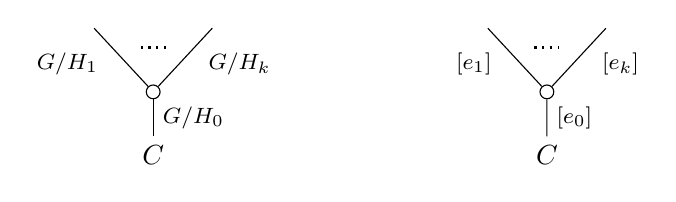
\begin{tikzpicture}
[grow=up,auto,level distance=2.3em,every node/.style = {font=\footnotesize},dummy/.style={circle,draw,inner sep=0pt,minimum size=1.75mm}]
	\node at (0,0) [font=\normalsize]{$C$}
		child{node [dummy] {}
			child{
			edge from parent node [swap,near end] {$G/H_k$} node [name=Kn] {}}
			child{
			edge from parent node [near end] {$G/H_1$}
node [name=Kone,swap] {}}
		edge from parent node [swap] {$G/H_0$}
		};
		\draw [dotted,thick] (Kone) -- (Kn) ;
	\node at (5,0) [font=\normalsize]{$C$}
		child{node [dummy] {}
			child{
			edge from parent node [swap,near end] {$[e_k]$} node [name=Kn] {}}
			child{
			edge from parent node [near end] {$[e_1]$}
node [name=Kone,swap] {}}
		edge from parent node [swap] {$[e_0]$}
		};
		\draw [dotted,thick] (Kone) -- (Kn) ;
\end{tikzpicture}
\]
We will then abbreviate $\sigma^i C = \sigma^{[e_i]} C$, and write $e_i$, $e_i'$ for the two edges of $\sigma^i C $ that degenerate the edge $e_i$ of $C$,
with $e_i$ denoting the inner edge and $e'_i$ the outer
edge.
\[
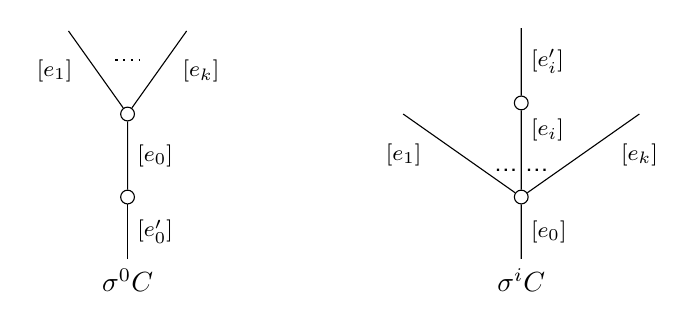
\begin{tikzpicture}
[grow=up,auto,level distance=3em,
every node/.style = {font=\footnotesize},
dummy/.style={circle,draw,inner sep=0pt,minimum size=1.75mm}]
	\node at (0,0) [font=\normalsize]{$\sigma^0 C$}
		child{node [dummy] {}
			child{node [dummy] {}
				child{
				edge from parent node [swap,near end] {$[e_k]$} node [name=Kn] {}}
				child{
				edge from parent node [near end] {$[e_1]$}
node [name=Kone,swap] {}}
			edge from parent node [swap] {$[e_0]$}}
		edge from parent node [swap] {$[e'_0]$}
		};
		\draw [dotted,thick] (Kone) -- (Kn) ;
	\node at (5,0) [font=\normalsize]{$\sigma^i C$}
		child{node [dummy] {}
			child{
			edge from parent node [swap,near end] {$[e_k]$} node [near start,inner sep=1pt,name=Kn] {}}
			child[level distance=3.4em]{node [dummy] {}
				child[level distance=2.7em]{
				edge from parent node [swap] {$[e'_i]$}
}
			edge from parent node [near end,swap] {$[e_i]$}
node [near start,inner sep=1pt,name=Kone,swap] {}
node [near start,inner sep=1pt,name=Kone1] {}}
			child{
			edge from parent node [near end] {$[e_1]$}
node [swap] {}
node [near start,inner sep=1pt,name=Kn1,swap]{}}
		edge from parent node [swap] {$[e_0]$}
		};
		\draw [dotted,thick] (Kone) -- (Kn) ;
		\draw [dotted,thick] (Kone1) -- (Kn1) ;
\end{tikzpicture}
\]
The $G$-tree $\sigma^i C$ then has an orbital inner face\footnote{See \cite[Defn. 2.16]{BP_edss} for a discussion of \textit{orbital} inner faces.}
$\sigma^i C - [e_i]$ obtained by removing $[e_i]$
as well as an orbital outer face obtained by removing $e'_i$,
which we denote $\sigma^i C - [e'_i]$.
Moreover, note that we have natural identifications
$C = \sigma^i C - [e_i]$,
$C = \sigma^i C - [e'_i]$.

In what follows, we will find it convenient to simplify notation by denoting maps $\Omega[T] \to X$,
where $T \in \Omega_G$ and $X \in \mathsf{dSet}^G$,
simply as $T \to X$.


\begin{definition}
	Let $X \in \mathsf{dSet}^G$ be a $G$-$\infty$-operad and $C$ a $G$-corolla with edge orbits
	$[e_0],\cdots,[e_k]$.
	
	Given two parallel operations 
	$f,g\colon C \rightrightarrows X$,
	we write $f \sim_i g$ if there exists a map
	$H \colon \sigma^i C \to X$ such that
\begin{itemize}
\item $f$ equals the restriction $H|_{\sigma^i C-[e'_i]}$;
\item $g$ equals the restriction $H|_{\sigma^i C-[e_i]}$;
\item the restriction $H|_{\sigma^i [e_i]}$
is the degeneracy $\sigma^i [e_i] \to [e_i] \to C \to X$.
\end{itemize}
\end{definition}


\begin{remark}\label{HOMOTBOUND REM}
	Note that if $f \sim_i g$ then it must be
	$f|_{\partial C} = g|_{\partial C}$.
\end{remark}


\begin{example}\label{EQUIVSIM EX}
	Let $G = \mathbb{Z}_{/2} = \{\pm 1\}$
	and consider the $G$-corolla with orbital and expanded representations as given on the left below.
\[
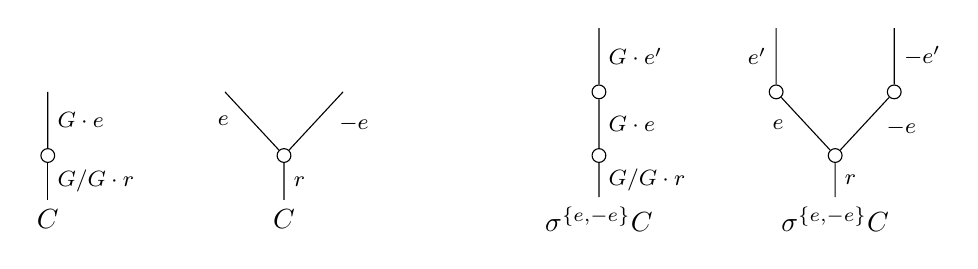
\begin{tikzpicture}
[grow=up,auto,level distance=2.3em,every node/.style = {font=\footnotesize},dummy/.style={circle,draw,inner sep=0pt,minimum size=1.75mm}]
	\node at (0,0) [font=\normalsize]{$C$}
		child{node [dummy] {}
			child{
			edge from parent node [swap] {$G \cdot e$}
node [name=Kone,swap] {}}
		edge from parent node [swap] {$G/G \cdot r$}
		};
	\node at (3,0) [font=\normalsize]{$C$}
		child{node [dummy] {}
			child{
			edge from parent node [swap,near end] {$-e$} node [name=Kn] {}}
			child{
			edge from parent node [near end] {$e$}
node [name=Kone,swap] {}}
		edge from parent node [swap] {$r$}
		};
	\node at (7,0) [font=\normalsize]{$\sigma^{\{e,-e\}} C$}
		child{node [dummy] {}
			child{node [dummy] {}
				child{
				edge from parent node [swap] {$G \cdot e'$}
node [swap] {}}
			edge from parent node [swap] {$G \cdot e$}
node [swap] {}}
		edge from parent node [swap] {$G/G \cdot r$}
		};
	\node at (10,0) [font=\normalsize]{$\sigma^{\{e,-e\}} C$}
		child{node [dummy] {}
			child{node [dummy] {}
				child{
				edge from parent node [swap] {$-e'$} node {}}
			edge from parent node [swap,near end] {$-e$} node {}}
			child{node [dummy] {}
				child{
				edge from parent node {$e'$}
node [swap] {}}
			edge from parent node [near end] {$e$}
node [swap] {}}
		edge from parent node [swap] {$r$}
		};
\end{tikzpicture}
\]
$C$ then has a single leaf $G$-edge orbit $[e] = G \cdot e$, so that for
$f,g \colon C \to X$ it is
$f \sim_1 g$
if there exists a dendrix
$H \colon \sigma^{\{e,-e\}}C \to X$
such that 
\begin{equation}\label{EQUIVHOMOT EQ}
	f = H|_{\sigma^{\{e,-e\}}C - \{e',-e'\}}
\qquad
	g = H|_{\sigma^{\{e,-e\}}C - \{e,-e\}}
\qquad
	H_{\sigma^e e}, H|_{\sigma^{-e}-e} \text{ are degenerate}.
\end{equation}
It is worthwhile to compare this equivariant relation with the relations obtained if one forgets the $G$-actions. Indeed, while \eqref{EQUIVHOMOT EQ} implicitly assumes that all of $f,g,H$ are $G$-equivariant,
by omitting that assumption one can reinterpret 
\eqref{EQUIVHOMOT EQ}
as defining a relation
$f \sim_{[e]} g$ between not necessarily $G$-equivariant maps $f,g \colon C \to X$.

A priori, $\sim_{[e]}$ relation differs from the 
non-equivariant 
$\sim_{e}$ and $\sim_{-e}$
relations obtained by regarding $C$ as a non-equivariant corolla.
However, for $f,g,H$ as in \eqref{EQUIVHOMOT EQ} one has
\begin{equation}\label{EQUIVSIM EQ}
f = H|_{\sigma^{\{e,-e\}}C - \{e',-e'\}}
\sim_e H|_{\sigma^{\{e,-e\}}C - \{e,-e'\}}
\sim_{-e} H|_{\sigma^{\{e,-e\}}C - \{e,-e\}} =g
\end{equation}
so that, by Lemma \ref{EQUIVI LEM}(b) below one has that
$f \sim_{[e]} g$ in fact implies
$f \sim_{e} g$. Moreover, the converse statement follows immediately by using degeneracies.

More generally, similar considerations show that the $\sim$ relations are compatible with restricting the $G$-actions.
\end{example}


\begin{lemma}\label{EQUIVI LEM}
	Let $X \in \mathsf{dSet}^G$ be a $G$-$\infty$-operad and $C$ a $G$-corolla with edge orbits
	$[e_0],\cdots,[e_k]$. Then:
\begin{itemize}
	\item[(a)] each of the relations $\sim_i$ is an equivalence relation;
	\item[(b)] all the equivalence relations $\sim_i$ coincide.
\end{itemize}
\end{lemma}

\begin{proof}
	We first address (a). 
	
	For the reflexive condition, one can take $H$ to be the degeneracy
	$\sigma^i C \xrightarrow{\sigma^i} C \xrightarrow{f} X$.
	
	For the symmetry and transitive conditions, consider the tree
	$\sigma^{ii} C$, which degenerates $[e_i]$ twice.
\[
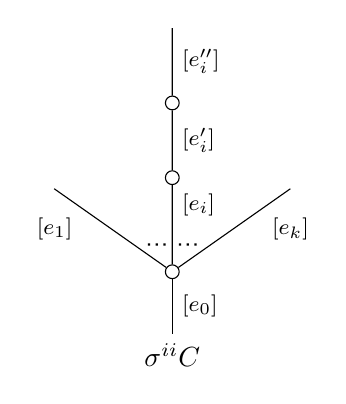
\begin{tikzpicture}
[grow=up,auto,level distance=3em,
every node/.style = {font=\footnotesize},
dummy/.style={circle,draw,inner sep=0pt,minimum size=1.75mm}]
	\node at (0,0) [font=\normalsize]{$\sigma^{ii} C$}
		child{node [dummy] {}
			child{
			edge from parent node [swap,near end] {$[e_k]$} node [near start,inner sep=1pt,name=Kn] {}}
			child[level distance=3.4em]{node [dummy] {}
				child[level distance=2.7em]{node [dummy] {}
					child[level distance=2.7em]{
					edge from parent node [swap] {$[e''_i]$}
}
				edge from parent node [swap] {$[e'_i]$}
}
			edge from parent node [near end,swap] {$[e_i]$}
node [near start,inner sep=1pt,name=Kone,swap] {}
node [near start,inner sep=1pt,name=Kone1] {}}
			child{
			edge from parent node [near end] {$[e_1]$}
node [swap] {}
node [near start,inner sep=1pt,name=Kn1,swap]{}}
		edge from parent node [swap] {$[e_0]$}
		};
		\draw [dotted,thick] (Kone) -- (Kn) ;
		\draw [dotted,thick] (Kone1) -- (Kn1) ;
\end{tikzpicture}
\]
Suppose $f \sim_i g$, and let 
$H \colon \sigma^{i} C \to X$ be the associated homotopy.
Define a map 
$\bar{H} \colon \Lambda^{[e_i]}_o[\sigma^{ii} C] \to X$ by
\[
	\bar{H}|_{\sigma^{ii}C - [e''_i]} = H,
		\qquad
	\bar{H}|_{\sigma^{ii}C - [e'_i]} = f \circ \sigma^i,
		\qquad
	\bar{H}|_{\sigma^{ii} [e_i]} = 
	f|_{[e_i]} \circ \sigma^{ii} =
	g|_{[e_i]} \circ \sigma^{ii}.
\]
Since the orbital inner horn inclusion
$\bar{H} \colon \Lambda^{[e_i]}_o[\sigma^{ii} C] \to \Omega[C]$
is $G$-inner anodyne by \cite[Prop. 3.13]{BP_edss},
$\bar{H}$ admits an extension $\widetilde{H} \colon \sigma^{ii}C \to X$.
The restriction $\bar{H}|_{\sigma^{ii}C - [e_i]}$ then provides the homotopy exhibiting $g \sim_i f$, and symmetry of $\sim_i$ follows.

Next, suppose $f \sim_i g$ and $g \sim_i h$, and let 
$H \colon \sigma^{i} C \to X$ and
$K \colon \sigma^{i} C \to X$ be be the associated homotopies.
Define a map 
$\bar{H} \colon \Lambda^{[e'_i]}_o[\sigma^{ii} C] \to X$ by
\[
	\bar{H}|_{\sigma^{ii}C - [e''_i]} = H,
		\qquad
	\bar{H}|_{\sigma^{ii}C - [e_i]} = K,
		\qquad
	\bar{H}|_{\sigma^{ii} [e_i]} = 
	f|_{[e_i]} \circ \sigma^{ii} =
	g|_{[e_i]} \circ \sigma^{ii} =
	h|_{[e_i]} \circ \sigma^{ii}.
\]
$\bar{H}$ again admits an extension $\widetilde{H} \colon \sigma^{ii}C \to X$, and the restriction $\bar{H}|_{\sigma^{ii}C - [e'_i]}$
provides the homotopy exhibiting $f \sim_i g$, so that transitivity of $\sim_i$.

We next turn to (b). Consider the tree $\sigma^{ij} C$ which degenerates $C$ once along each of $[e_i]$ and $[e_j]$.
\[
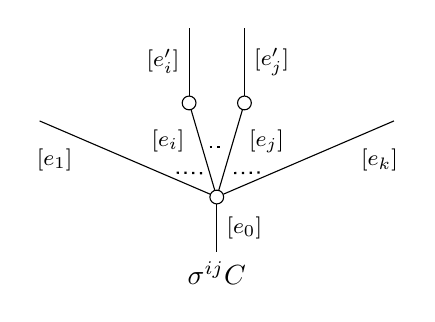
\begin{tikzpicture}
[grow=up,auto,level distance=2.75em,
every node/.style = {font=\footnotesize},
dummy/.style={circle,draw,inner sep=0pt,minimum size=1.75mm}]
	\node at (0,0) [font=\normalsize]{$\sigma^{ij} C$}
		child{node [dummy] {}
			child{
			edge from parent node [swap,near end] {$[e_k]$} node [near start,inner sep=1pt,name=Kn] {}}
			child[level distance=3.4em,sibling distance=2em]{node [dummy] {}
				child[level distance=2.7em]{
				edge from parent node [swap] {$[e'_j]$}
}
			edge from parent node [very near end,swap] {$[e_j]$}
node [near start,inner sep=1pt,name=Kone,swap] {}
node [inner sep=1pt,name=Kn2] {}}
			child[level distance=3.4em,sibling distance=2em]{node [dummy] {}
				child[level distance=2.7em]{
				edge from parent node {$[e'_i]$}
}
			edge from parent node [very near end] {$[e_i]$}
node [inner sep=1pt,name=Kone2,swap] {}
node [near start,inner sep=1pt,name=Kone1] {}}
			child{
			edge from parent node [near end] {$[e_1]$}
node [swap] {}
node [near start,inner sep=1pt,name=Kn1,swap]{}}
		edge from parent node [swap] {$[e_0]$}
		};
		\draw [dotted,thick] (Kn) -- (Kone) ;
		\draw [dotted,thick] (Kone1) -- (Kn1) ;
		\draw [dotted,thick] (Kone2) -- (Kn2) ;
\end{tikzpicture}
\]
Suppose $f \sim_i g$ with $H \colon \sigma^{i} C \to X$ the associated homotopy.
Define a map 
$\bar{H} \colon \Lambda^{[e_i]}_o[\sigma^{ij} C] \to X$ by
\[
	\bar{H}|_{\sigma^{ij}C - [e'_j]} = H,
		\qquad
	\bar{H}|_{\sigma^{ij}C - [e_j]} = f \circ \sigma^i,
		\qquad
	\bar{H}|_{\sigma^{ij}C - [e'_i]} = f \circ \sigma^j.
\]
Yet again, $\bar{H}$ admits an extension $\widetilde{H} \colon \sigma^{ij}C \to X$, and the restriction $\bar{H}|_{\sigma^{ij}C - [e_i]}$
provides a homotopy exhibiting $g \sim_j f$. (b) now follows.
\end{proof}

In light of Lemma \ref{EQUIVI LEM},
given parallel operation $f,g \colon C \rightrightarrows X$ with 
$C$ a $G$-corolla and $X$ a $G$-$\infty$-operad,
we will henceforth write $f \sim g$ whenever $f \sim_i g$ for some (and thus all) $i$.
We now extend the $\sim$ relation.

\begin{definition}\label{XTENDSIM DEF}
	Let $T \in \Omega_G$ be a $G$-tree
	and $X \in \mathsf{dSet}^G$ be a 
	$G$-$\infty$-operad.
	
	Given dendrices $x,y\colon T \to X$ we write
	$x \sim y$ if there are equivalences of restrictions
	$x|_{T_v} \sim y|_{T_v}$ for all $G$-vertices
	$v \in \boldsymbol{V}_G(T)$.
	
	Further, we define $\mathsf{ho}(X)(T) = X(T)/\sim$.
\end{definition}

\begin{proposition}
Let $X \in \mathsf{dSet}^G$ be a $G$-$\infty$-operad. Then the assignment 
		$T \mapsto \mathsf{ho}(X)(T)$
		is a contravariant functor in $T \in \Omega_G$, i.e.
		$\mathsf{ho}(X)\in \mathsf{dSet}_G$.
\end{proposition}


\begin{proof}
	It suffices to show that the $\sim$ equivalence relations are compatible with the generating classes of maps in $\Omega_G$, namely
	degeneracies, inner faces, outer faces, and quotient maps.
	
	The cases of degeneracies and outer faces are obvious. In the case of quotients, 
	since any quotient $\bar{T} \to T$ of $G$-trees induces quotients on $G$-vertices, it suffices to consider the case of a quotient
	$\bar{C} \xrightarrow{\pi} C$ of $G$-corollas.
	But it is then straightforward to check that if a homotopy exhibiting $f \sim_0 g$ also induces a homotopy exhibiting 
	$f \circ \pi \sim_0 g \circ \pi$
	(notably, the same needs not be true for the relations $f \sim_i g$ when $0<i$, 
	in which case the exhibiting homotopy 
	may instead exhibit a string of relations 
	$f \circ \pi \sim \cdots \sim g \circ \pi$
	as in \eqref{EQUIVSIM EQ}).

It remains to address the most interesting case,
that inner faces. Since inner faces can be factored as composites of inner faces that collapse a singe inner edge orbit,
it suffices to consider the case of faces
$D \to T$ where $T$ has a single inner edge orbit; that is,
we can assume that there are $G$-corollas
$C_1$, $C_2$ such that 
$T = C_1 \amalg_{[e_i]} C_2$ and
$D = T - [e_i]$, as illustrated below.
\[
\begin{tikzpicture}
[grow=up,auto,level distance=3em,
every node/.style = {font=\footnotesize},
dummy/.style={circle,draw,inner sep=0pt,minimum size=1.75mm}]
	\node at (0,0) [font=\normalsize]{$C_1$}
		child{node [dummy] {}
			child{
			edge from parent node [swap,near end] {} node [near start,inner sep=1pt,name=Kn] {}}
			child[level distance=3.4em]{node {}
			edge from parent node [near end,swap] {$[e_i]$}
node [near start,inner sep=1pt,name=Kone,swap] {}
node [near start,inner sep=1pt,name=Kone1] {}}
			child{
			edge from parent node [near end] {}
node [swap] {}
node [near start,inner sep=1pt,name=Kn1,swap]{}}
		edge from parent node [swap] {$[e_0]$}
		};
		\draw [dotted,thick] (Kone) -- (Kn) ;
		\draw [dotted,thick] (Kone1) -- (Kn1) ;
	\node at (4,0) [font=\normalsize]{$C_2$}
		child{node [dummy] {}
			child{
			edge from parent node [swap,near end] {} node [name=Kn] {}}
			child{
			edge from parent node [near end] {}
node [name=Kone,swap] {}}
		edge from parent node [swap] {$[e_i]$}
		};
		\draw [dotted,thick] (Kone) -- (Kn) ;
	\node at (9,0) [font=\normalsize]{$T$}
		child{node [dummy] {}
			child{
			edge from parent node [swap,near end] {} node [near start,inner sep=1pt,name=Kn] {}}
			child[level distance=3.4em]{node [dummy] {}
				child{
				edge from parent node [swap,near end] {} node [name=Kn2] {}}
				child{
				edge from parent node [near end] {}
node [name=Kone2,swap] {}}
			edge from parent node [near end,swap] {$[e_i]$}
node [near start,inner sep=1pt,name=Kone,swap] {}
node [near start,inner sep=1pt,name=Kone1] {}}
			child{
			edge from parent node [near end] {}
node [swap] {}
node [near start,inner sep=1pt,name=Kn1,swap]{}}
		edge from parent node [swap] {$[e_0]$}
		};
		\draw [dotted,thick] (Kone) -- (Kn) ;
		\draw [dotted,thick] (Kone1) -- (Kn1) ;
		\draw [dotted,thick] (Kone2) -- (Kn2) ;
\end{tikzpicture}
\]
The claim is now that if
$x,y \colon T \to X$ are such that
$x|_{C_1} \sim y|_{C_1}$ and
$x|_{C_2} \sim y|_{C_2}$
then it is also 
$x|_{D} \sim y|_{D}$.
This will follow from the next two claims:
\begin{itemize}
\item[(i)] if $x,y \colon T \to X$ are such that
$x|_{C_1} = y|_{C_1}$ and
$x|_{C_2} = y|_{C_2}$
then $x|_{D} \sim y|_{D}$;
\item[(ii)]
given $x \colon T \to X$, $f\colon C_1 \to X$ and
$g \colon C_2 \to X$ such that
$f \sim x|_{C_1}$, $g \sim x|_{C_2}$,
there exists
$y \colon T \to X$ such that
$y|_{C_1} = f$, $y|_{C_2} = g$ and
$y|_D = x|_D$.
\end{itemize}
To show (i) and (ii), consider the degeneracies
$\sigma^0 T$ and $\sigma^i T$ pictured below.
\[
\begin{tikzpicture}
[grow=up,auto,level distance=3em,
every node/.style = {font=\footnotesize},
dummy/.style={circle,draw,inner sep=0pt,minimum size=1.75mm}]
	\node at (0,0) [font=\normalsize]{$\sigma^0 T$}
		child{node [dummy] {}
		child{node [dummy] {}
			child{
			edge from parent node [swap,near end] {} node [near start,inner sep=1pt,name=Kn] {}}
			child[level distance=3.4em]{node [dummy] {}
				child{
				edge from parent node [swap,near end] {} node [name=Kn2] {}}
				child{
				edge from parent node [near end] {}
node [name=Kone2,swap] {}}
			edge from parent node [near end,swap] {$[e_i]$}
node [near start,inner sep=1pt,name=Kone,swap] {}
node [near start,inner sep=1pt,name=Kone1] {}}
			child{
			edge from parent node [near end] {}
node [swap] {}
node [near start,inner sep=1pt,name=Kn1,swap]{}}
		edge from parent node [swap] {$[e_0]$}}
		edge from parent node [swap] {$[e'_0]$}
		};
		\draw [dotted,thick] (Kone) -- (Kn) ;
		\draw [dotted,thick] (Kone1) -- (Kn1) ;
		\draw [dotted,thick] (Kone2) -- (Kn2) ;
	\node at (6,0) [font=\normalsize]{$\sigma^i T$}
		child{node [dummy] {}
			child{
			edge from parent node [swap,near end] {} node [near start,inner sep=1pt,name=Kn] {}}
			child[level distance=3.4em]{node [dummy] {}
			child{node [dummy] {}
				child{
				edge from parent node [swap,near end] {} node [name=Kn2] {}}
				child{
				edge from parent node [near end] {}
node [name=Kone2,swap] {}}
			edge from parent node [swap] {$[e'_i]$}}
			edge from parent node [near end,swap] {$[e_i]$}
node [near start,inner sep=1pt,name=Kone,swap] {}
node [near start,inner sep=1pt,name=Kone1] {}}
			child{
			edge from parent node [near end] {}
node [swap] {}
node [near start,inner sep=1pt,name=Kn1,swap]{}}
		edge from parent node [swap] {$[e_0]$}
		};
		\draw [dotted,thick] (Kone) -- (Kn) ;
		\draw [dotted,thick] (Kone1) -- (Kn1) ;
		\draw [dotted,thick] (Kone2) -- (Kn2) ;
\end{tikzpicture}
\]
Given $x,y$ as in (i), one can now build a map
$H \colon \Lambda_o^{[e_i]}[\sigma^0 T] \to X$ by
\[
	H|_{\sigma^0 T - [e_0]} = x,
\qquad
	H|_{\sigma^0 T - [e'_0]} = y,
\qquad
	H|_{\sigma^0 C_1} = 
	x|_{C_1} \circ \sigma^0 = 
	y|_{C_1} \circ \sigma^0.
\]
Letting $\widetilde{H}\colon \sigma^0 T \to X$
be an extension of $H$,
the restriction $H|_{\sigma^0 T - [e_i]}$
provides the desired homotopy 
$x|_{D} \sim y|_{D}$, showing (i).


Lastly, let $x,f,g$ be as in (ii), 
and let
$K \colon \sigma^i C_1 \to X$ exhibit the relation
$f \sim_i x|_{C_1}$
and 
$ \bar{K} \colon \sigma^i C_2 \to X$
exhibit the relation
$x|_{C_2} \sim_i g$ (note the reversed order).
Now build the map
$H \colon \Lambda_o^{[e'_i]}[\sigma^i T] \to X$ by
\[
	H|_{\sigma^i T - [e_i]} = x,
\qquad
	H|_{\sigma^i C_1} = K,
\qquad
	H|_{\sigma^i C_2} = \bar{K}.
\]
Again letting 
$\widetilde{H} \colon \sigma^i T \to X$,
the restriction 
$\widetilde{H}|_{\sigma^i T - [e'_i]}$
provides the required $y \colon T \to X$,
showing (ii) and finishing the proof.
\end{proof}


\begin{corollary}\label{HOOPUNIV COR}
Let $X \in \mathsf{dSet}^G$ be a $G$-$\infty$-operad. Then
	\begin{itemize}
	\item[(a)] $\mathsf{ho}(X)\in \mathsf{dSet}_G$ is a genuine equivariant operad, i.e. it satisfies the strict right lifting condition against the Segal core inclusions
	$Sc[T] \to \Omega[T]$ for $T \in \Omega_G$;
	\item[(b)] the quotient map
	$\upsilon_{\**}X \to \mathsf{ho}(X)$ is the universal map from $\upsilon_{\**}X$ to a genuine equivariant operad.
	\end{itemize}
\end{corollary}

\begin{proof}
	Note first that by Remark \ref{HOMOTBOUND REM}
	any map 	$Sc[T] \to \mathsf{ho}(X)$ admits a factorization 
	$Sc[T] \to \upsilon_{\**}X \xrightarrow{q} \mathsf{ho}(X)$.
	
	The right lifting property for $\mathsf{ho}(X)$
	against the maps $Sc[T] \to \Omega[T]$
	is then automatic from the lifting property for $X$.

	For strictness,	
	note that Definition \ref{XTENDSIM DEF}
	can be reinterpreted as saying that
	a pair of dendrices $\Omega[T] \rightrightarrows X$
	give rise to the same point of 
	$\mathsf{ho}(X)$, i.e. 
	the composites 
	$\Omega[T] \rightrightarrows X \xrightarrow{q}
	\mathsf{ho}(X)$ coincide, 
	iff the composites 
	$Sc[T] \to \Omega[T] \rightrightarrows X \xrightarrow{q}
	\mathsf{ho}(X)$ coincide, showing strictness, and thus (a).
		
	For (b), since $\mathsf{ho}(X)$ is a quotient of
	$\upsilon_{\**} X$, it suffices to show that any map
	from $F \colon \upsilon_{\**}X \to Y$ with $Y$ a genuine equivariant operad must also enforce the $\sim$ relation.
	For a $G$-corolla $C$ and
	$f,g\colon C \to X$ such that 
	$H \colon \sigma^i C \to X$ exhibits
	$f \sim_i g$, 
	the strict lifting condition for $Y$
	shows that the maps
	$F\circ H \colon \sigma^i C \to Y$,
	$f \circ \sigma^i \colon \sigma^i C \to Y$
	must coincide, and thus that
	$F(f)=F(g)$.
	The further claim that $F$ respects equivalences
	of general pair of dendrices $T \rightrightarrows X$
	is immediate from Definition \ref{XTENDSIM DEF}.
\end{proof}



{\color{red} HERE}

The following is the analogue of \cite[Prop. 4.8]{CM13b}.

\begin{proposition}
      \label{HOOPID_PROP}
Let $\mathcal{O} \in \mathsf{sOp}^G$
be a fibrant. 
Then there is a natural isomorphism of genuine equivariant operads
\begin{equation}\label{HOOPID EQ}
ho(hcN(\mathcal{O})) \xrightarrow{\simeq}
\pi_0 \left( \upsilon_{\**} N\mathcal{O} \right).
\end{equation}
\end{proposition}


\begin{proof}
      By \cite[Prop. 5.9]{BP_edss}, $\pi_0(\upsilon_{\**}N\O)$ is a genuine equivariant operad,
      and the existence of the map in \eqref{HOOPID EQ}
      will be an application of
      Corollary \ref{HOOPUNIV COR}(b).

Firstly,
note that we have the following, naturally in $T \in \Omega_G$.
\[
\upsilon_{\**}hcN(\O)(T)
\simeq
\mathsf{sOp}^G(W_!\Omega[T],\O)
\simeq
\mathsf{sdSet}^G(N W_!\Omega[T],N \O)
\simeq 
\mathsf{sdSet}_G(\upsilon_{\**}N W_!\Omega[T],\upsilon_{\**}N \O)
\]
where the second and third identifications use the fact that 
$N\colon \mathsf{Op} \to \mathsf{dSet}$ and $\upsilon_{\**} \colon \dSet^G \to \dSet_G$
are fully faithful inclusions. 
But now one has a map
\begin{align*}
  \mathsf{sdSet}_G(\upsilon_{\**}N W_!\Omega[T],\upsilon_{\**}N \O)
  & \to
    \mathsf{sdSet}_G(\upsilon_{\**}N W_!\Omega[T],\pi_0\upsilon_{\**}N \O)
  \\ & \simeq
       \mathsf{dSet}_G(\pi_0 \upsilon_{\**}  N W_!\Omega[T],\pi_0\upsilon_{\**}N \O)
  \\ & \simeq
       \mathsf{dSet}_G(\upsilon_{\**}\Omega[T],\pi_0\upsilon_{\**}N \O)
  \\ & =
       (\pi_0\upsilon_{\**}N \O)(T)
\end{align*}
so altogether we obtain a map
$\upsilon_{\**}hcN(\O) \to \pi_0 \upsilon_{\**} N \O$
and hence, by Corollary \ref{HOOPUNIV COR},
the desired map 
\[ho(hcN(\O)) \to \pi_0 \upsilon_{\**} N \O\]
Moreover, both of these are quotients of $\upsilon_{\**}hcN(\O)$,
so to prove that the map is an isomorphism one needs only show that any two parallel operations $C \rightrightarrows hcN \O$ of $\upsilon_{\**}hcN(\O)$
that are identified in 
$\pi_0 \upsilon_{\**} N \O$
were already identified in 
$ho(hcN(\O))$.
But this now follows immediately from the pushout from Proposition \ref{WLEFTQPUSH PROP}
\[
\begin{tikzcd}
	\Omega(C) \otimes_{\mathsf{F}}
	\partial \Delta[1]
	\ar{r} \ar{d}
&
	W_! \left(\partial \Omega[C \star \eta]\right) 
	\ar{d}
\\
	\Omega(C) \otimes_{\mathsf{F}}
	\Delta[1]
	\ar{r}
&
	W(C \star \eta)
\end{tikzcd}
\]
\end{proof}


come back

\begin{lemma}
      \label{HOXISOFIB_LEM}
      $ho(X)$ detects isofibrations between $G$-$\infty$-operads.
\end{lemma}
\begin{proof}
      Recall that $f \colon X \to Y$ in $\dSet^G$ is an isofibration iff
      \(
      \tau j^{\**}i_{\**}(f) = \tau i_G^{\**}\upsilon_{\**}(f)
      \)
      is levelwise an isofibration in $\Cat$.
      \[
            \begin{tikzcd}
                  \dSet^G \arrow[r, "i_{\**}"] \arrow[d, "\upsilon_{\**}"']
                  &
                  \dSet^{\mathsf O_G^{op}} \arrow[d, "j^{\**}"]
                  \\
                  \dSet_G \arrow[r, "i_G^{\**}"]
                  &
                  \Set^{\mathsf O_G^{op}} \arrow[r, "\tau"]
                  &
                  \Cat^{\mathsf O_G^{op}}
            \end{tikzcd}
      \]
      We see that $i_G^{\**} \upsilon_{\**} X \to i_G^{\**} ho(X)$ is again a universal map to a (levelwise) strict Segal object,
      but then the universal property of the $(\tau, N)$-adjunction implies
      \[
            N\tau j^{\**}i_{\**}X \simeq i_G^{\**} ho(X).
      \]
      The result follows.
\end{proof}

\begin{remark}
      \label{W!_LEFTQ_REM}
      Proposition \ref{HOOPID_PROP} and Lemma \ref{HOXISOFIB_LEM}
      provide a second finish to the proof of Proposition \ref{W!_LEFTQ_PROP}:
      $hcN(f)$ is an isofibration iff
      $i_G^{\**}ho(hcN(f)) = i_G^{\**} \pi_0(\upsilon_{\**}(N\O))$ is so,
      but $N \colon \sOp^G \to \mathsf{PreOp}^G$ is right Quillen
      and $i_G^{\**}\pi_0\upsilon_{\**}$ detects isofibrations in $\mathsf{PreOp}^G$.
\end{remark}

      

% \begin{remark} % ---------- OLD W!_LEFTQ_REM ----------
%       This gives us a second finish to the proof of Proposition \ref{W!_LEFTQ_PROP}:
%       $hcN(f)$ is an $\F$-fibration iff $\tau (kj)^{\**} \upsilon_{\**} h c N(f)$ is,
%       but
%       \[
%             +            \tau (kj)^{\**} \upsilon_{\**} hcN(f) =
%             \tau N \tau (kj)^{\**} \upsilon_{\**} hcN(f) \simeq
%             \tau (kj)^{\**} ho( hcN(f) ) \simeq
%             \tau (kj)^{\**} \pi_0 \upsilon_{\**} N \O =
%             \pi_0 j^{\**} i_{\**} f,
%       \]
%       where the last equality follows from the diagram below.
%       \[
%             \begin{tikzcd}[column sep = scriptsize]
%                   \sOp^G \arrow[d, equal] \arrow[rrr, "i_{\**}"]
%                   &&&
%                   \sOp^{\mathsf O_{\F_1}^{op}} \arrow[d, "N"'] \arrow[r, "j^{\**}"]
%                   &
%                   \mathsf{sCat}^{\mathsf O_{\F_1}^{op}} \arrow[d, "N"'] \arrow[r, "\pi_0"]
%                   &
%                   \Cat^{\mathsf O_{\F_1}^{op}} \arrow[d, "N"'] \arrow[r, equal]
%                   &
%                   \Cat^{\mathsf O_{\F_1}^{op}} \arrow[d, equal]
%                   \\
%                   \sOp^G \arrow[d, equal] \arrow[r, "N"]
%                   &
%                   \mathsf{sdSet}^G \arrow[d, equal] \arrow[rr, "i_{\**}"]
%                   &&
%                   \mathsf{sdSet}^{\mathsf O_{\F_1}^{op}} \arrow[d, equal] \arrow[r, "j^{\**}"]
%                   &
%                   \mathsf{ssSet}^{\mathsf O_{\F_1}^{op}} \arrow[r, "\pi_0"]
%                   &
%                   \sSet^{\mathsf O_{\F_1}^{op}} \arrow[d, equal] \arrow[r, "\tau"]
%                   &
%                   \Cat^{\mathsf O_{\F_1}^{op}} \arrow[d, equal]
%                   \\
%                   \sOp^G \arrow[d, equal] \arrow[r, "N"]
%                   &
%                   \mathsf{sdSet}^G \arrow[d, equal] \arrow[r, "\upsilon_{\**}"]
%                   &
%                   \mathsf{sdSet}_G \arrow[d, equal] \arrow[r, "k^{\**}"]
%                   &
%                   \mathsf{sdSet}^{\mathsf O_{\F_1}^{op}} \arrow[r, "\pi_0"]
%                   &
%                   \dSet^{\mathsf O_{\F_1}^{op}} \arrow[d, equal] \arrow[r, "j^{\**}"]
%                   &
%                   \sSet^{\mathsf O_{\F_1}^{op}} \arrow[d, equal] \arrow[r, "\tau"]
%                   &
%                   \Cat^{\mathsf O_{\F_1}^{op}} \arrow[d, equal]
%                   \\
%                   \sOp^G \arrow[r, "N"]
%                   &
%                   \mathsf{sdSet}^G \arrow[r, "\upsilon_{\**}"]
%                   &
%                   \mathsf{sdSet}_G \arrow[r, "\pi_0"]
%                   &
%                   \dSet_G \arrow[r, "k^{\**}"]
%                   &
%                   \dSet^{\mathsf O_{\F_1}^{op}} \arrow [r, "j^{\**}"]
%                   &
%                   \sSet^{\mathsf O_{\F_1}^{op}} \arrow[r, "\tau"]
%                   &
%                   \Cat^{\mathsf O_{\F_1}^{op}}
%             \end{tikzcd}
%       \]
%       But $f \in \sOp^G$ is an isofibration iff
%       $\pi_0 j^{\**} i_{\**} f$ is a level isofibration, finishing the proof.
% \end{remark}
















\newpage

\bibliography{biblio3}{}
\bibliographystyle{amsalpha2}



\end{document}


%%% Local Variables:
%%% mode: latex
%%% TeX-master: t
%%% End:
